\documentclass[12pt]{article}
\usepackage[utf8]{inputenc}
\usepackage{amsmath}
\usepackage{graphicx}
\usepackage{listings}
\usepackage{verbatim}
\usepackage{float}
\usepackage{xcolor}
\usepackage{subcaption}
\usepackage[english]{babel}
\usepackage{caption}
\usepackage{hyperref}
\usepackage{biblatex}
\addbibresource{report.bib}
\usepackage{setspace}
\usepackage{wrapfig}
\usepackage{lipsum}
\usepackage{amssymb}
\linespread{1.25}
\usepackage[a4paper, total={6in, 9in}]{geometry}
\DeclareMathOperator*{\E}{\mathbb{E}}


\hypersetup{
    colorlinks,
    linkcolor={red!50!black},
    citecolor={blue!50!black},
    urlcolor={blue!80!black}
}
\definecolor{codegreen}{rgb}{0,0.6,0}
\definecolor{codegray}{rgb}{0.5,0.5,0.5}
\definecolor{codepurple}{rgb}{0.58,0,0.82}
\definecolor{backcolour}{rgb}{0.95,0.95,0.92}
\definecolor{dkgreen}{rgb}{0,0.6,0}
\definecolor{gray}{rgb}{0.5,0.5,0.5}
\definecolor{mauve}{rgb}{0.58,0,0.82}

\lstdefinestyle{mystyle}{
    backgroundcolor=\color{backcolour},
    commentstyle=\color{codegreen},
    keywordstyle=\color{magenta},
    numberstyle=\tiny\color{codegray},
    stringstyle=\color{codepurple},
    basicstyle=\ttfamily\footnotesize,
    breakatwhitespace=false,
    breaklines=true,
    captionpos=b,
    keepspaces=true,
    numbers=left,
    numbersep=5pt,
    showspaces=false,
    showstringspaces=false,
    showtabs=false,
    tabsize=2
}

\lstset{style=mystyle}
\title{Project 1\\ Regression analysis and resampling methods}
\author{Filip Severin von der Lippe}
\date{\today}
\begin{document}
\maketitle
Github repository containing code and further instuction on how to reproduce the results of this report: \url{https://github.com/Fslippe/FYS-STK4155/tree/main/project1}
\begin{abstract}
  Central methods in machine learning include regression analysis and resampling methods, which lately have made a great impact on our understanding of the world around us. To gain a fundamental understanding of how these methods work, we will do regression analysis using ordinary least squares, Ridge and Lasso regression together with the resampling methods Bootstrap and Cross validation. By using data generated by the Franke function and real topography data we have gained an insight in how these methods perform in different circumstances and we have ended up showing that the Ridge method generally gives us the most accurate results. Furthermore we have looked into the performance of the Lasso method, and found that there are certain important steps in the implementation of, together with computational limits in how well this method performs.
\end{abstract}
\newpage
\tableofcontents
\section{Introduction}
In this project we will study regression and resampling methods by using them to analyze real topography data and data generated from the Franke function. Both the Franke function and topography data are two dimensional systems taking in coordinates in $x$ and $y$ direction which gives us a way of generalizing our analyzing methods to work for both. We will use ordinary least squares, Ridge and Lasso regression in our study of our data and do comparisons to try finding the optimal model for the different datasets. We will implement cross validation and Bootstrap to analyze our results to gain the best possible predictions. This will be done in the form of both looking at the bias variance tradeoff, and a mean square error analysis using cross validation to find optimal parameters and polynomial degrees for our datasets. First will a description of both our data and methods together with the necessary theory be presented. This involves a derivation of the ordinary least squares method and following variances and expectation values of the parameters computed, a derivation of the bias variance tradeoff, and otherwise descriptions on how and why we implement the different methods used in our analysis. Later we will present our results where we first will look into our data from the Franke function and in the end the real topography data. Lastly we will discuss our results including weaknesses of our implementations and possibilities for further research.
\section{Method}
Our fist step is to set up our data for analysis. We start by implementing the Franke function which is a sum of four exponentials:
\begin{align*}
  f(x,y) &= \frac{3}{4 }\exp\left(- \frac{(9x -2 )^2}{4} - \frac{(9y-2)^2}{4}\right) +\frac{3}{4}\exp{\left(-\frac{(9x+1)^2}{49}- \frac{(9y+1)}{10}\right)} \\
&+\frac{1}{2}\exp{\left(-\frac{(9x-7)^2}{4} - \frac{(9y-3)^2}{4}\right)} -\frac{1}{5}\exp{\left( -(9x-4)^2 - (9y-7)^2\right) }
\end{align*}
By using this function we generate our data by using ($n+1\times n+1$) points in a meshgrid for $x$ and $y$ in the interval [0,1]. This gives us a function value of ($n+1 \times n+1$) to which we add a stochastic noise $\epsilon \sim N(0,\sigma^2)$ for a chosen standard deviation $\sigma$. When describing our data later in this report we refer to $n$ steps and $\sigma$ which are used to produce the data as described above. This leaves us with our data described by the Franke function plus some noise $\epsilon$:
\begin{align*}
  \boldsymbol{z} = f(\boldsymbol{x}) + \boldsymbol{\epsilon}
\end{align*}
This can also be assumed from some real data, based on the existence of a continuous function $f$ and normal distributed error $\epsilon$.

For the Regression method ordinary least squares we have made theese assumptions which gives us an approximation to the above equation where we minimize $(\boldsymbol{z} - \boldsymbol{\tilde{z}})^2$ to give us the matrix equation:
\begin{align*}
  \boldsymbol{\tilde{z}} = \boldsymbol{X}\boldsymbol{\beta}
\end{align*}
for a chosen design matrix $\boldsymbol{X}$ of some degree $N$ with the dimensions $(n+1)\times (N+1)(N+2)/2$ and $\beta$ with the dimensions $(N+1)(N+2)/2$ for our case where we choose the design matrix to follow a $x$ and $y$ dependent polynomial on the form:
\begin{align*}
  \boldsymbol{X} = \begin{bmatrix}
    1 & x_0 & y_0 & x_0^2 & x_0y_0 & y_0^2 & \hdots &x_0^N & y_0^N \\
    1 & x_1 & y_1 & x_1^2 & x_1y_1 & y_1^2 &\hdots& x_1^N & y_1^N \\
    \vdots & \vdots & \vdots & \vdots & \vdots &\vdots & &\vdots & \vdots \\
    1 & x_n & y_n & x_n^2 & x_ny_n & y_n^2 &\hdots& x_n^N & y_n^N
\end{bmatrix}
, \quad
\boldsymbol{\beta} =
\begin{bmatrix}
  \beta_0 \\
  \beta_1 \\
  \vdots \\
  \beta_n
\end{bmatrix}
\end{align*}

This approximation gives us a new way of describing our dataset in terms of $\boldsymbol{\tilde{z}}$ instead of $f(\boldsymbol{x})$.
\begin{align*}
  \boldsymbol{z} = \sum_{j=0}^{n-1}\beta_jx_i^j + \epsilon_i
\end{align*}
This is the same as the following matrix equation:
\begin{align*}
  \boldsymbol{z} = \boldsymbol{X}\boldsymbol{\beta} + \boldsymbol{\epsilon} = \boldsymbol{\tilde{z}} + \boldsymbol{\epsilon}
\end{align*}
This means that the element $i$ is given by:
\begin{align*}
  z_i = \epsilon_i + \sum_j x_{ij}\beta_j
\end{align*}
Which gives the expectation value of the element $i$ in $\boldsymbol{z}$:
\begin{align*}
  E(z_i) = E(\epsilon_i + \sum_j x_{ij}\beta_j)
\end{align*}
Since we already know or have assumed that $\boldsymbol{\epsilon}$ is normally distributed with the expectation value 0 ($E(\epsilon_i)=0$), this gives us:
\begin{align*}
  E(z_i) = E(\epsilon_i) + E(\sum_j x_{ij}\beta_j) = \sum_jE(x_{ij}\beta_j)
\end{align*}
$x_{ij}$ and $\beta_j$ are values and not distributions which means they have themselves as expectation values:
\begin{align*}
    E(z_i) = \sum_jx_{ij}\beta_j = \boldsymbol{X_i}_*\boldsymbol{\beta}
\end{align*}

To find the variance we again recognize that $\boldsymbol{X}\boldsymbol{\beta}$ follow no distribution which leaves us with the variance of $\boldsymbol{z}$ equaling the variance of $\boldsymbol{\epsilon}$ which is given as $\sigma^2$:
\begin{align*}
  \text{Var}(\boldsymbol{z}) = \text{Var}(\boldsymbol{X}\boldsymbol{\beta} + \boldsymbol{\epsilon}) = \text{Var}(\boldsymbol{\epsilon}) = \sigma^2
\end{align*}

$\boldsymbol{\tilde{z}}$ is defined through the minimization of the mean square error $(\boldsymbol{z} - \boldsymbol{\tilde{z}})^2$ which for $\boldsymbol{\tilde{z}} = \boldsymbol{X}\boldsymbol{\beta}$ translates to the minimization of the cost function:
\begin{align*}
  C(\boldsymbol{\beta}) = \frac{1}{ n}\{(\boldsymbol{z}- \boldsymbol{X}\boldsymbol{\beta}^T\boldsymbol{z}- \boldsymbol{X}\boldsymbol{\beta})\}
\end{align*}
Where we take the derivative with respect to $\boldsymbol{\beta}$ and solve for $\boldsymbol{\beta}$ where the derivative is 0 to find the minimum:
\begin{align*}
  \frac{\partial C(\boldsymbol{\beta})}{\partial \boldsymbol{\beta}} = \boldsymbol{X}^T (\boldsymbol{z}- \boldsymbol{X}\boldsymbol{\beta}) =0
\end{align*}
\begin{align*}
  \boldsymbol{X}^T\boldsymbol{z} = \boldsymbol{X}^T \boldsymbol{X}\boldsymbol{\beta}
\end{align*}
We assume that $\boldsymbol{X}^T\boldsymbol{X}$ is invertible which gives us the the optimal $\boldsymbol{\beta}$:
\begin{align*}
  \boldsymbol{\tilde{\beta}} = (\boldsymbol{X}^T\boldsymbol{X})^{-1} \boldsymbol{X}^T\boldsymbol{z}
\end{align*}
We can now find the expectation value for the optimal $\boldsymbol{\tilde{\beta}}$:
\begin{align*}
  E(\boldsymbol{\tilde{\beta}}) &= E[(\boldsymbol{X}^T\boldsymbol{X})^{-1} \boldsymbol{X}^T\boldsymbol{z}] = E[(\boldsymbol{X}^T\boldsymbol{X})^{-1} \boldsymbol{X}^T(\boldsymbol{X}\boldsymbol{\beta} + \boldsymbol {\epsilon} )] \\
  &=  (\boldsymbol{X}^T\boldsymbol{X})^{-1} \boldsymbol{X}^TE[(\boldsymbol{X}\boldsymbol{\beta} + \boldsymbol {\epsilon} )] \\ &= (\boldsymbol{X}^T\boldsymbol{X})^{-1} \boldsymbol{X}^T\boldsymbol{X}\boldsymbol{\beta} \\&=  \boldsymbol{\beta}
\end{align*}
Here we see that the expectation value of our optimal parameter is the parameter $\boldsymbol{\beta}$.

We now find the variance of the optimal parameter:
\begin{align*}
  \text{Var}(\boldsymbol{\tilde{\beta}}) &= \text{Var}[(\boldsymbol{X}^T\boldsymbol{X})^{-1} \boldsymbol{X}^T(\boldsymbol{X}\boldsymbol{\beta} + \boldsymbol {\epsilon} )] \\
  &= \text{Var}[(\boldsymbol{X}^T\boldsymbol{X})^{-1} \boldsymbol{X}^T\boldsymbol {\epsilon} ]
\end{align*}
For a matrix $A$ we have Var$(\boldsymbol{AX}+b) = \boldsymbol{A}\text{Var}(\boldsymbol{X})\boldsymbol{A}^T$ which gives us:
\begin{align*}
  \text{Var}(\boldsymbol{\tilde{\beta}})&=(\boldsymbol{X}^T\boldsymbol{X})^{-1}\boldsymbol{X}^T\text{Var}[ {\boldsymbol{\epsilon}} ]((\boldsymbol{X}^T\boldsymbol{X})^{-1})^T\boldsymbol{X} \\  &=
  (\boldsymbol{X}^T\boldsymbol{X})^{-1}\boldsymbol{X}^T\text{Var}[ {\boldsymbol{\epsilon}} ](\boldsymbol{X}^T)^{-1}\boldsymbol{X}^{-1}\boldsymbol{X} \\&=
   (\boldsymbol{X}^T\boldsymbol{X})^{-1}\text{Var}[ {\boldsymbol{\epsilon}} ]
\end{align*}

All this gives us a base to compute the optimal $\beta$ and in turn give us an OLS prediction for our real function $f$.

\subsection{Splitting and scaling of data}
A central part of regression analysis is to scale and split our data to avoid both overfitting and avoid the MSE to contain the intercept. In our case of the Franke function we have $x,y \in [0,1]$ which gives $z$ data on the same order which may indicate that a scaling is unnecessary. This expectation comes from that our data does not include any extreme values of any other order  that may negatively influence our predictors. In other words, scaling of data is normally what we do to get the data as equal to each other or on the order as our Franke data already is. To see if this expectation is valid, we test it by comparing our non-scaled data to mean scaled data where we have subtracted the mean. Here we only perform a mean scale and not the more normal standard scale because this would include a divide of the standard deviation. Since our data is in between 0 and 1 already will such a scaling only increase the magnitude of our values because of a standard deviation of less than 1.

To avoid overfitting we perform a 80-20 percent split into train and test data. We use the train data to train the model or in other words find the $\beta$ parameters. To predict we use the trained model together with the test data which leaves us with a more generalized prediction not only working for the data we have at hand, but also other data coming from the same source. This can be explained by for example a model trained so well with a design matrix $\boldsymbol{X}$ of an infinite degree that its prediction follows every noisy outlier. This would match the data at hand very well and give us an extremely low MSE, but give us high MSE for prediction made with new data which were not used to train the model. To test this we look at both MSE and R squared for $\boldsymbol{X}$ of different degrees for a trained model using train data, where we compare predictions using the same train data, to predictions using test data.
\subsection{Mean squared error and R squared}
For different design matrices $\boldsymbol{X}$ with different polynomial degrees we can calculate the mean squared error and R squared. This is done using the following equations where we define $z$ as our test data containing $n+1$ points.

\begin{align*}
  MSE(\boldsymbol{z}, \boldsymbol{\tilde{z}}) = \frac{1}{n }\sum_{i=0}^{n}(z_i- \tilde{z}_i)^2
\end{align*}
\begin{align*}
  R^2(\boldsymbol{z}, \boldsymbol{\tilde{z}}) = 1 - \frac{\sum_{i=0}^{n}(z_i- \tilde{z}_i)^2}{\sum_{i=0}^{n}(z_i- \bar{z}_i)^2}
\end{align*}
For the mean value:
\begin{align*}
  \bar{z} = \frac{1}{n }\sum_{i=0}^{n}z_i
\end{align*}

\subsection{Bootstrap and the Bias-variance trade-off}
To study the bias-variance trade-off we first implement the bootstrap resampling technique. This is done by resampling our train data $n_B$ times with replacement. That means we gain $n_B$ new samples that may be unique but still only contain values from the original sample. This in turn is used to compute our predictions leaving us with a total of $n_B$ different predictions. From these we get following the central limit theorem under the assumption that our $n_B$ datasets are independent and identically distributed a mean prediction value following $\frac{1}{n}\sum_i \boldsymbol{z}_i$ and a standard deviation of $\sigma/\sqrt{m}$ where $\sigma$ is the standard deviation of our added noise in the case of using the Franke function.

By looking back at the cost function which is minimized in order to find our optimal parameters $\boldsymbol{\beta}$ we can derive an expression for the bias and variance.

\begin{align*}
  C(\boldsymbol{X}, \boldsymbol{\beta}) = \frac{1 }{n }\sum_ {i=0}^{n-1}(z_i - \tilde{z}_i)^2 = \E[(\boldsymbol{z}- \boldsymbol{\tilde{z}})^2]
\end{align*}
By the definition of our data $z = f +\epsilon$ we rewrite the costfunction:
\begin{align*}
  \E[(\boldsymbol{z}- \boldsymbol{\tilde{z}})^2] &= \E[(f + \epsilon - \tilde{z} + \E[\tilde{z}]- \E[\tilde{z}])^2] \\                                             &= \E[f^2 + \epsilon^2 + \tilde{z}^2 + 2\E[\tilde{z}]^2 \\
                                                 &+ 2f\epsilon + 2f\tilde{z} + 2f\E[\tilde{z}] - 2f\E[\tilde{z}]\\
                                                 &+ 2\epsilon\tilde{z} + 2\epsilon \E[\tilde{z}] - 2\epsilon \E[\tilde{z}]\\
                                                 &+ 2\tilde{z}\E[\tilde{z}] - 2\tilde{z}\E[\tilde{z}] -2\E[\tilde{z}]^2]\\
                                                 &= \E[(f-\E[\Tilde{z}])^2] + \E[\epsilon^2] + \E[( \E[\Tilde{z}] - \Tilde{z} )^2] \\
                                                 &+ 2(f-\E[\tilde{z}])\E[\epsilon]+2\E[\epsilon]\E[(\E[\tilde{z}]-\tilde{z} )] \\
                                                &+ 2(f-\E[\tilde{z}])\E[( \E[\tilde{z}] - \tilde{z} )]
\end{align*}
By using that $\epsilon \sim N(0,1)$ we have $\E[\epsilon] = 0$ and Var$[\epsilon] = \E[\epsilon^2]- \E[\epsilon]^2 = \E[\epsilon^2]=\sigma^2$ from this we get:
\begin{align*}
  \E[(\boldsymbol{z}- \boldsymbol{\tilde{z}})^2] &=\E[(f -\E[\tilde{z}])^2] +\E[( \tilde{z} -\E[\tilde{z}])^2]  + \sigma^2+ 2(f-\E[\tilde{z}])\E[\E[\tilde{z}] -\tilde{z}]\\
  &=\E[(f -\E[\tilde{z}])^2]  + \E[( \tilde{z} -\E[\tilde{z}])^2]+\sigma^2\\
  &= \E[(f -\E[\tilde{z}])^2]  + \text{var}[\tilde{f}] + \sigma^2
\end{align*}
We see that the first term is (Bias$[\tilde{f}])^2$ but we are left with a problem to compute it because $f$ is unknown. To be able to find the bias we look at the computeable $E[(y - \E[\tilde{y}])^2]$ and the relation $z= f + \epsilon$:
\begin{align*}
  E[(y - \E[\tilde{y}])^2] &= \E[(\epsilon + f - \E[\tilde{y}])^2] \\
                           &= \E[\epsilon^2] + \E[(f- \E[\tilde{y}])^2] + \E[-2\epsilon(f- \E[\tilde{y}])] \\
\end{align*}
We recognize once again that we can remove terms that have $\epsilon$ in them from $\E[\epsilon] = 0$ giving us:
\begin{align*}
  \E[(f- \E[\tilde{y}])^2] =   E[(y - \E[\tilde{y}])^2] - \sigma^2
\end{align*}
And we end up with the the relation:
\begin{align*}
  \E[(\boldsymbol{z}- \boldsymbol{\tilde{z}})^2] &= (\text{Bias}[\tilde{f}])^2 + \text{var}{\tilde{f}} + \sigma^2\\
   &=   \left((\text{Bias}[\tilde{y}])^2 - \sigma^2\right) + \text{var}[\tilde{f}] + \sigma^2
\end{align*}
In other words we compute the correct bias for our models by subtracting the variance of our noise. In the case of our topography data where we do not know $\sigma$ we leave the bias without the subtraction of $\sigma^2$

\subsection{Cross validation}
To further investigate our model we implement the cross validation resampling method. Together with the already implemented bootstrap method we now have a possibility to optimize our predictions by choosing a design matrix that reduces our models' mean squared errors. The cross validation method takes in data and splits it up in $k$ equally sized sets where one set is used as test data while the rest is used as train data. For every fold a mean squared error is computed before the model reruns with another set as test data. This process happens over and over until all $k$ sets have been used as test data. This gives a total of $k$ folds. Since our data is ordered and not chaotic we shuffle it before the splits are performed. We can see why this is necessary in the $k$-fold visualization in figure \ref{fig:k_fold} where we would without a shuffle have $x,y$ and $z$ that are not representative of the whole dataset but rather small intervals of values. We can imagine how not shuffling the data would have consequences in an extreme case where the first split of the first $k$-fold in the figure below only contained values around 0 while the rest contained values around 1. That would leave us with high computed mean squared errors for especially some of the folds which would in turn give us bad predictions for the MSE.
\begin{figure}[H]
  \centering
  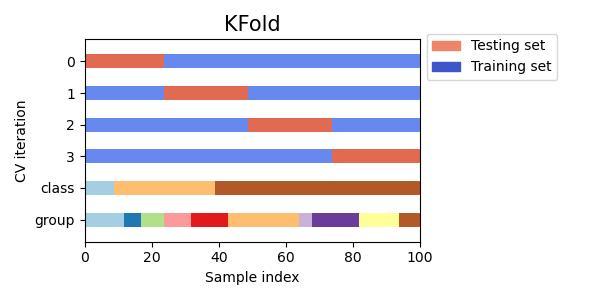
\includegraphics[width=.7\textwidth]{../figures/cv_kfold.png}
  \caption{A visualization of the splits of the data performed in cross validation. Here we see 4 $k$-folds which gives a total of 4 splits and iterations. Picture from sklearn's description of its cross validation method \cite{cv}}
  \label{fig:k_fold}
\end{figure}

\subsection{Study of $\lambda$ dependence for ridge and lasso regression}
To get the best possible predictions of our datasets we also implement lasso and ridge regression. These two methods are unlike OLS dependent on a regularization parameter $\lambda$ where we have to compute which value of this parameter that optimizes these two models. Similar to OLS we perform cross validation to find which degree of design matrix reduces the mean squared error of our predictions, only that we for ridge and lasso find the best $\lambda$ at the same time. This is because we for one degree would have one optimal $\lambda$ and for another degree have another. We therefore compute one cross validation for different values of $\lambda$ parameters for each degree. The degree and $\lambda$ giving the smallest MSE is then used for further predictions. We also look into how different choices of $\lambda$ influences our $\beta$ parameters by plotting the parameters for different $\lambda$ parameters for a chosen design matrix of degree 5 .


\subsection{Study of topography data}
After studying the Franke function with added noise we look at real topography data from the mountains close to Stavanger in Norway. We perform the same analysis as we did with the Franke function except that we now assume that our data already contain some noise $\epsilon \sim N(0, \sigma^2)$ with an unknown standard deviation $\sigma$. We first standard scale our data by subtracting the mean and dividing by the standard deviation computed from the data:
\begin{align*}
  z_{scaled} = \frac{z-\bar{z}}{\hat{\sigma}_z}
\end{align*}
Our regression analysis will then be used to try to compute how the topography at the location actually looks. Since the imported data includes  $3601 \times1801$ data points which would require more powerful hardware or atleast take a significant time to analyze, we choose an interesting location of indexes 100 to 141 in both directions and slice the data for every second index. That means we are left with input data of lower resolution, but at the same time it enables us to do an analysis over a greater area.
\section{Results}
\subsection{Franke function}
\subsubsection{Scaling of data}
We first look if there is a need of scaling our data or not. As seen in figure \ref{fig:compare_scale} we have plotted the absolute difference between the computed MSE and $R^2$ for different polynomial degrees using ordinary least squares. Here we have used input data of $n=30$ steps and $\sigma=0.2$.
\begin{figure}[H]
  \begin{subfigure}{.5\textwidth}
    \centering
    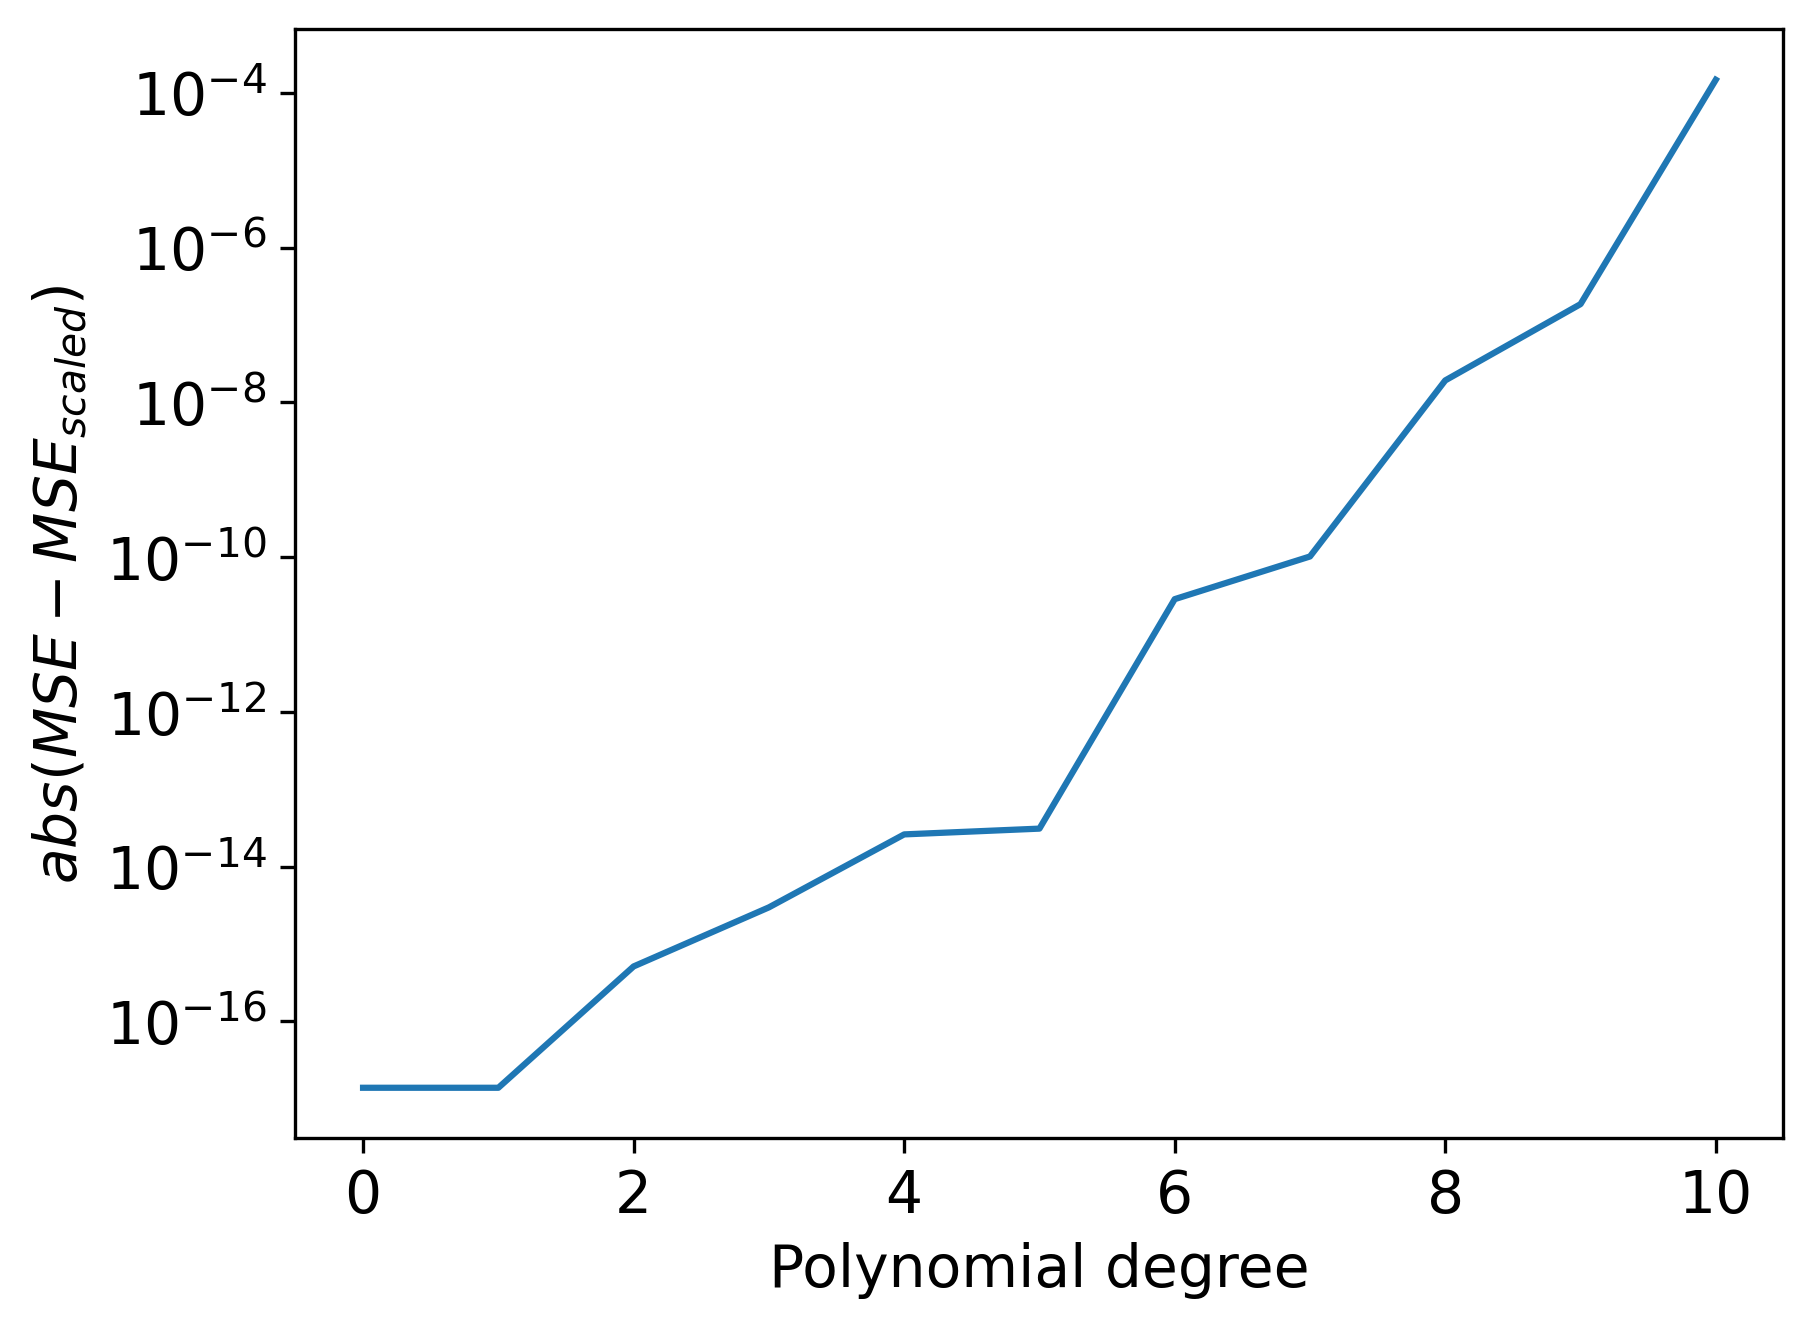
\includegraphics[width=\textwidth]{../figures/compare_scale_mse.png}
    \caption{$MSE$}
    \label{fig:}
  \end{subfigure}
  \begin{subfigure}{.5\textwidth}
    \centering
    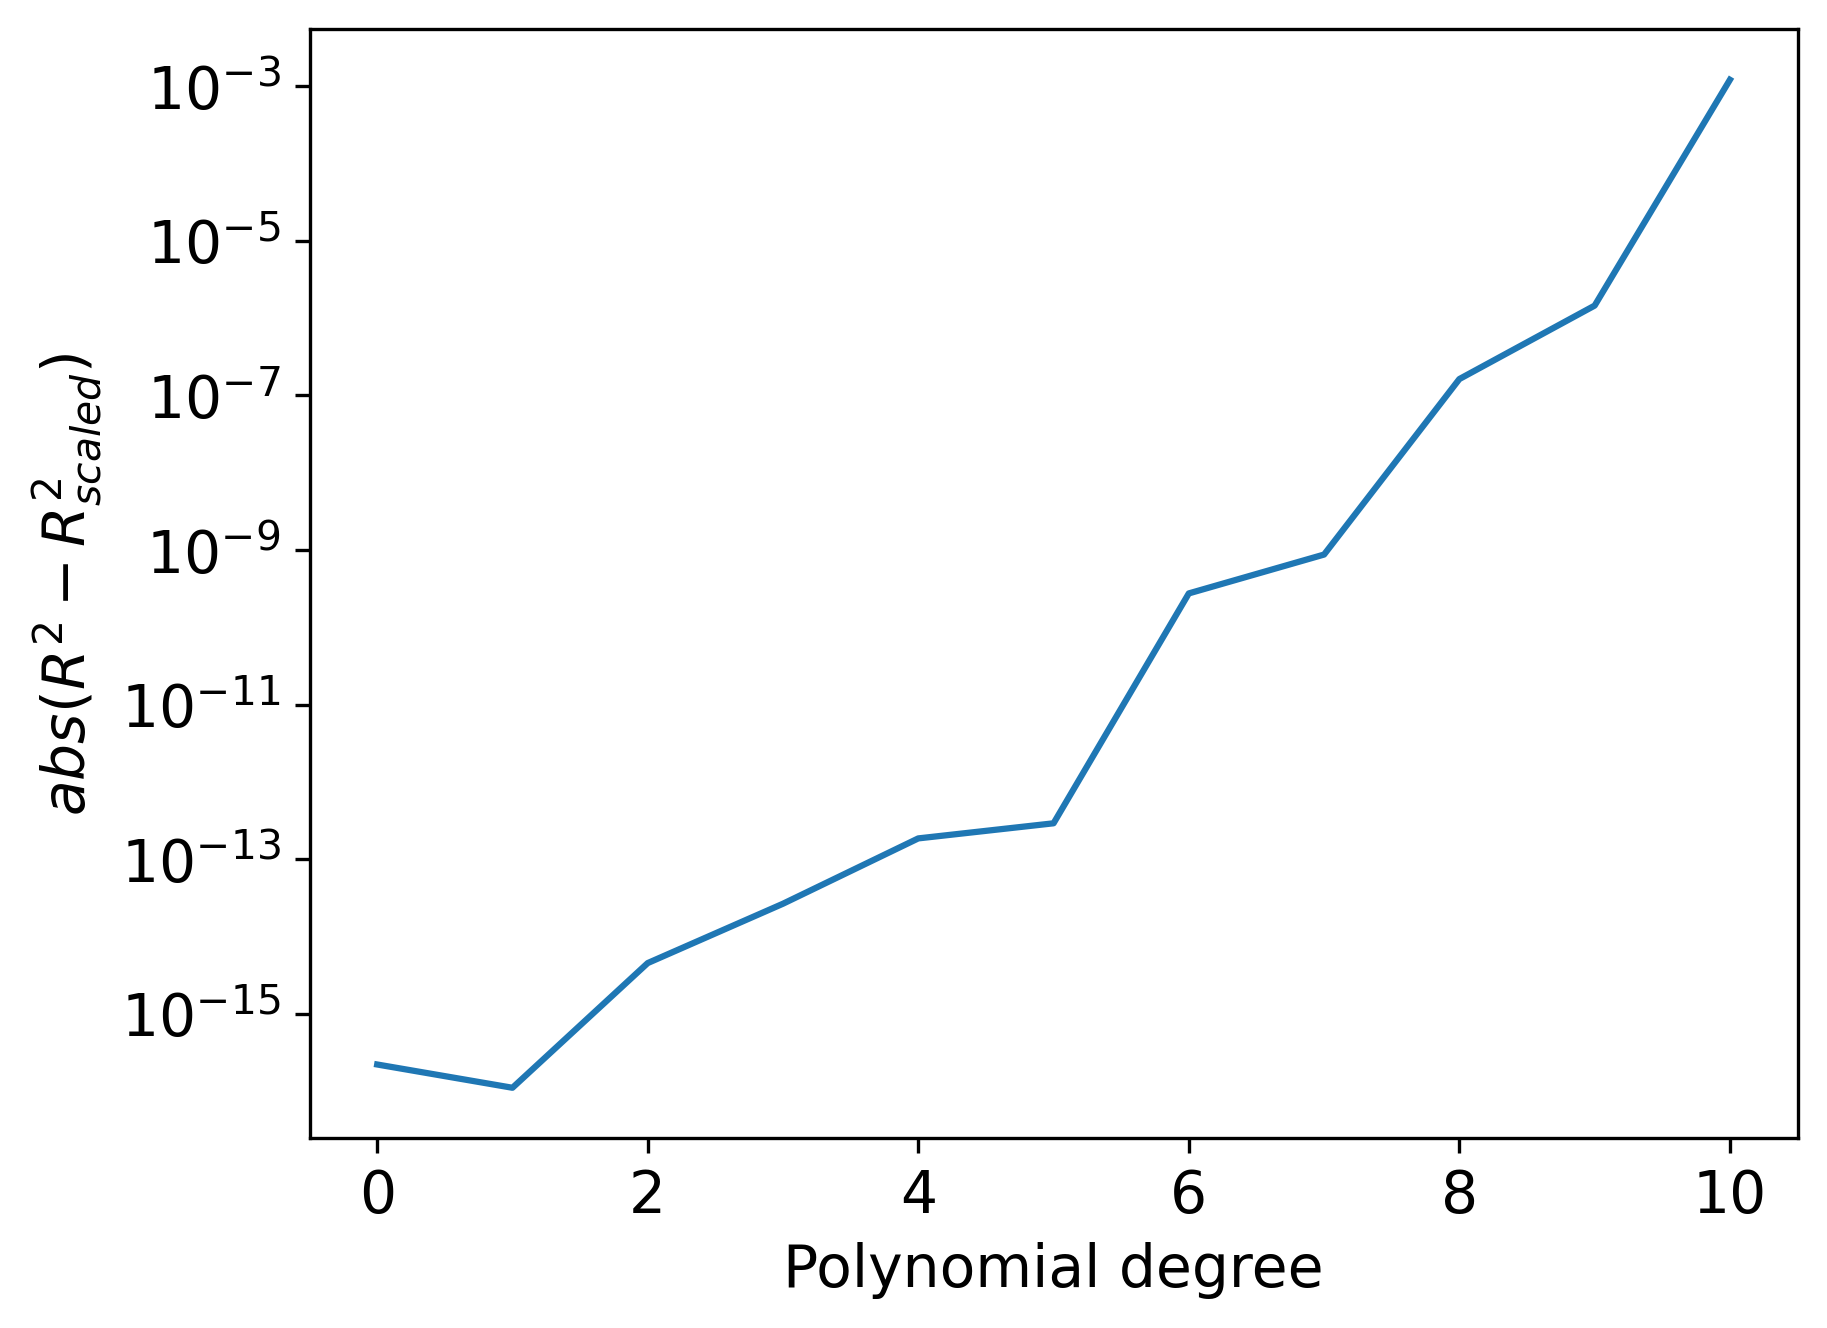
\includegraphics[width=\textwidth]{../figures/compare_scale_r2.png}
    \caption{$R^2$}
    \label{fig:}
  \end{subfigure}
  \caption{Comparison of MSE and $R^2$ between scaled and non-scaled data}
  \label{fig:compare_scale}
\end{figure}
We see that the difference between the scaled and non-scaled data are small, especially for lower polynomial degrees, which may indicate that scaling of our data is unnecessary.

\subsubsection{MSE, $R^2$ and splitting of data}
We continue with our non-scaled data and are still using the OLS method to look at how the mean square error and R squared behave for design matrices of different degrees. Underneath in figure \ref{fig:r2_mse_5} we see them both plotted for design matrices up to a degree of 5 for $n=30$ steps and $\sigma=0.2$.
\begin{figure}[H]
  \begin{subfigure}{.5\textwidth}
    \centering
    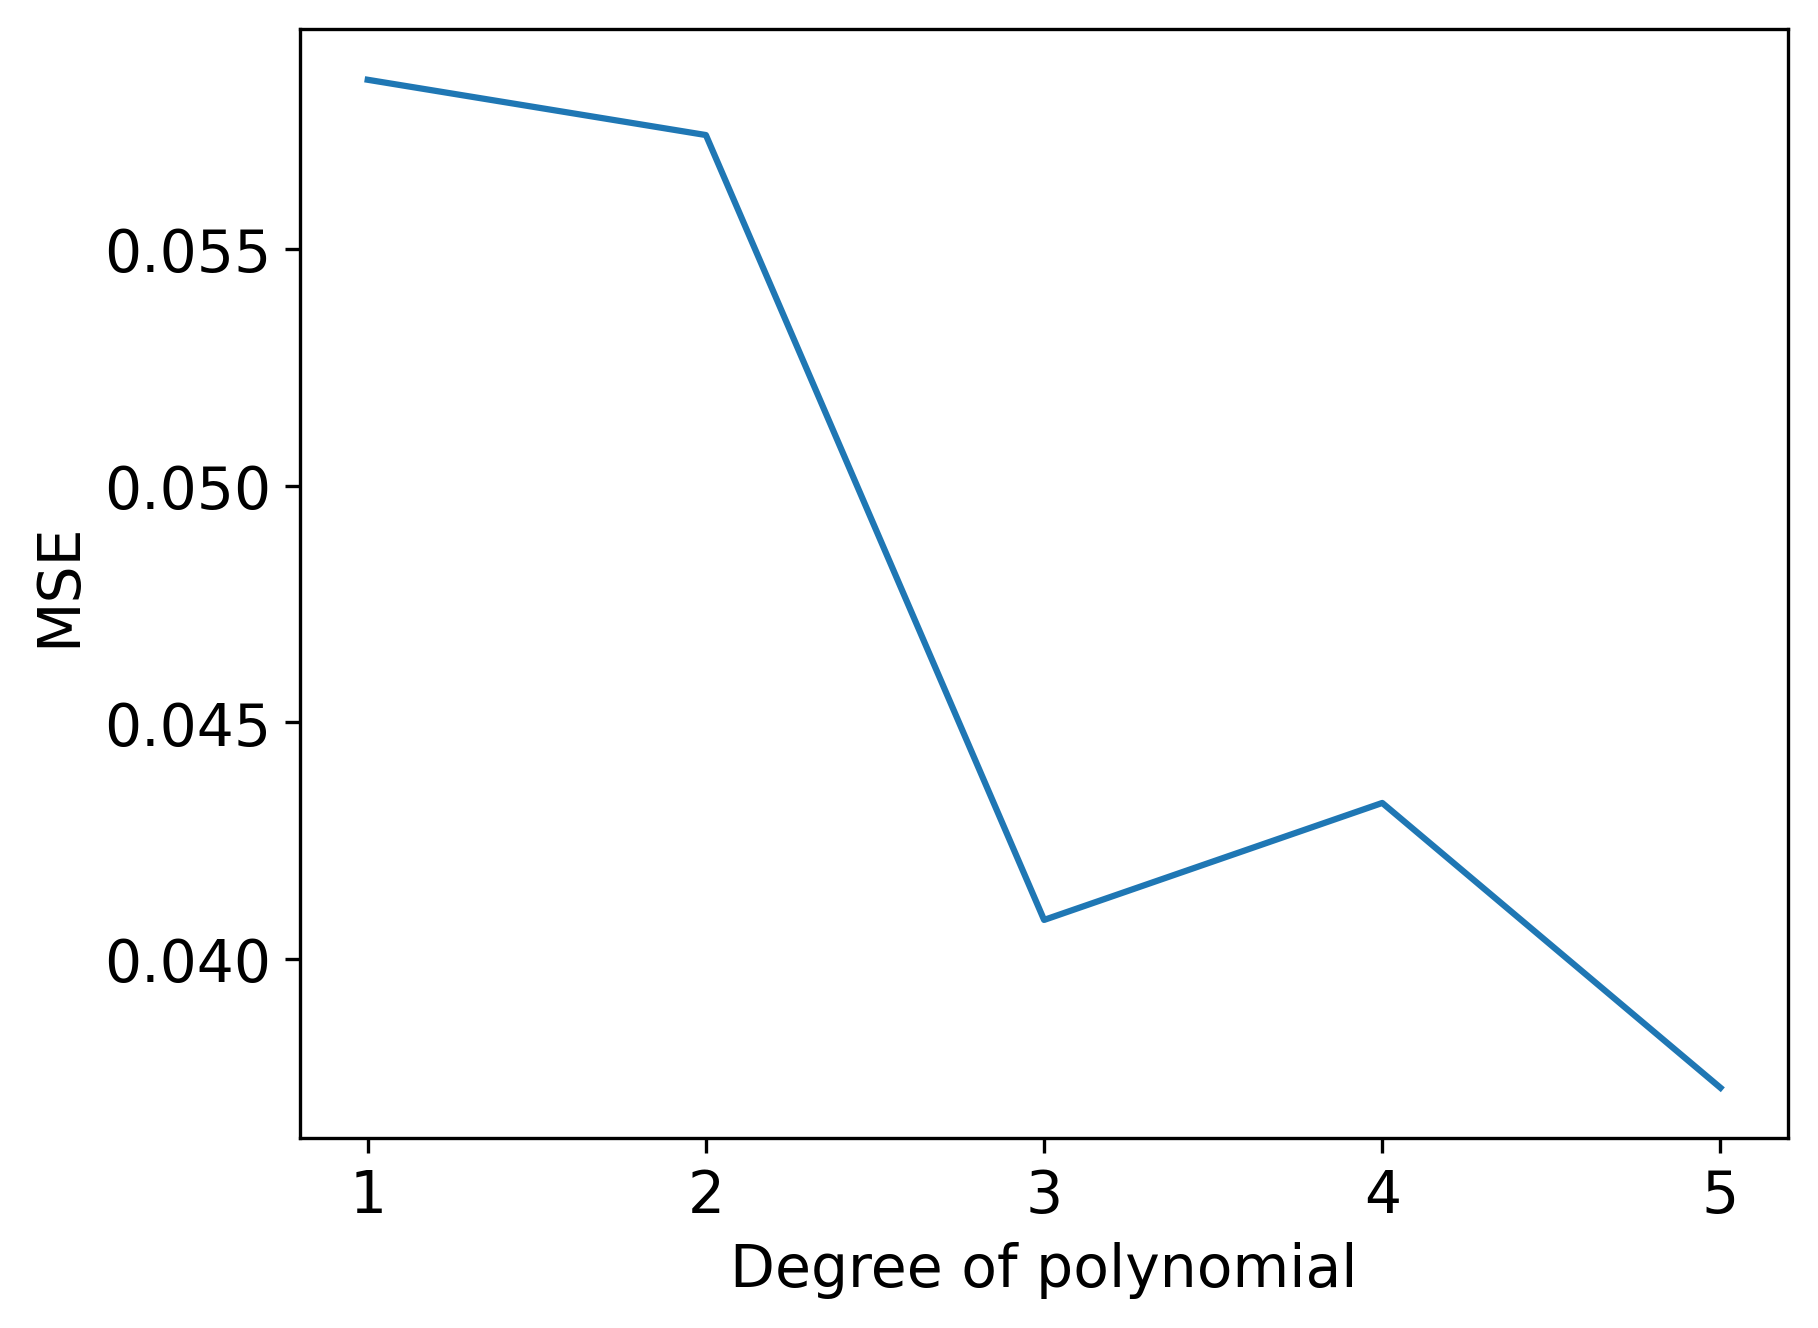
\includegraphics[width=\textwidth]{../figures/mse_ols_5.png}
    \caption{$MSE$}
    \label{fig:}
  \end{subfigure}
  \begin{subfigure}{.5\textwidth}
    \centering
    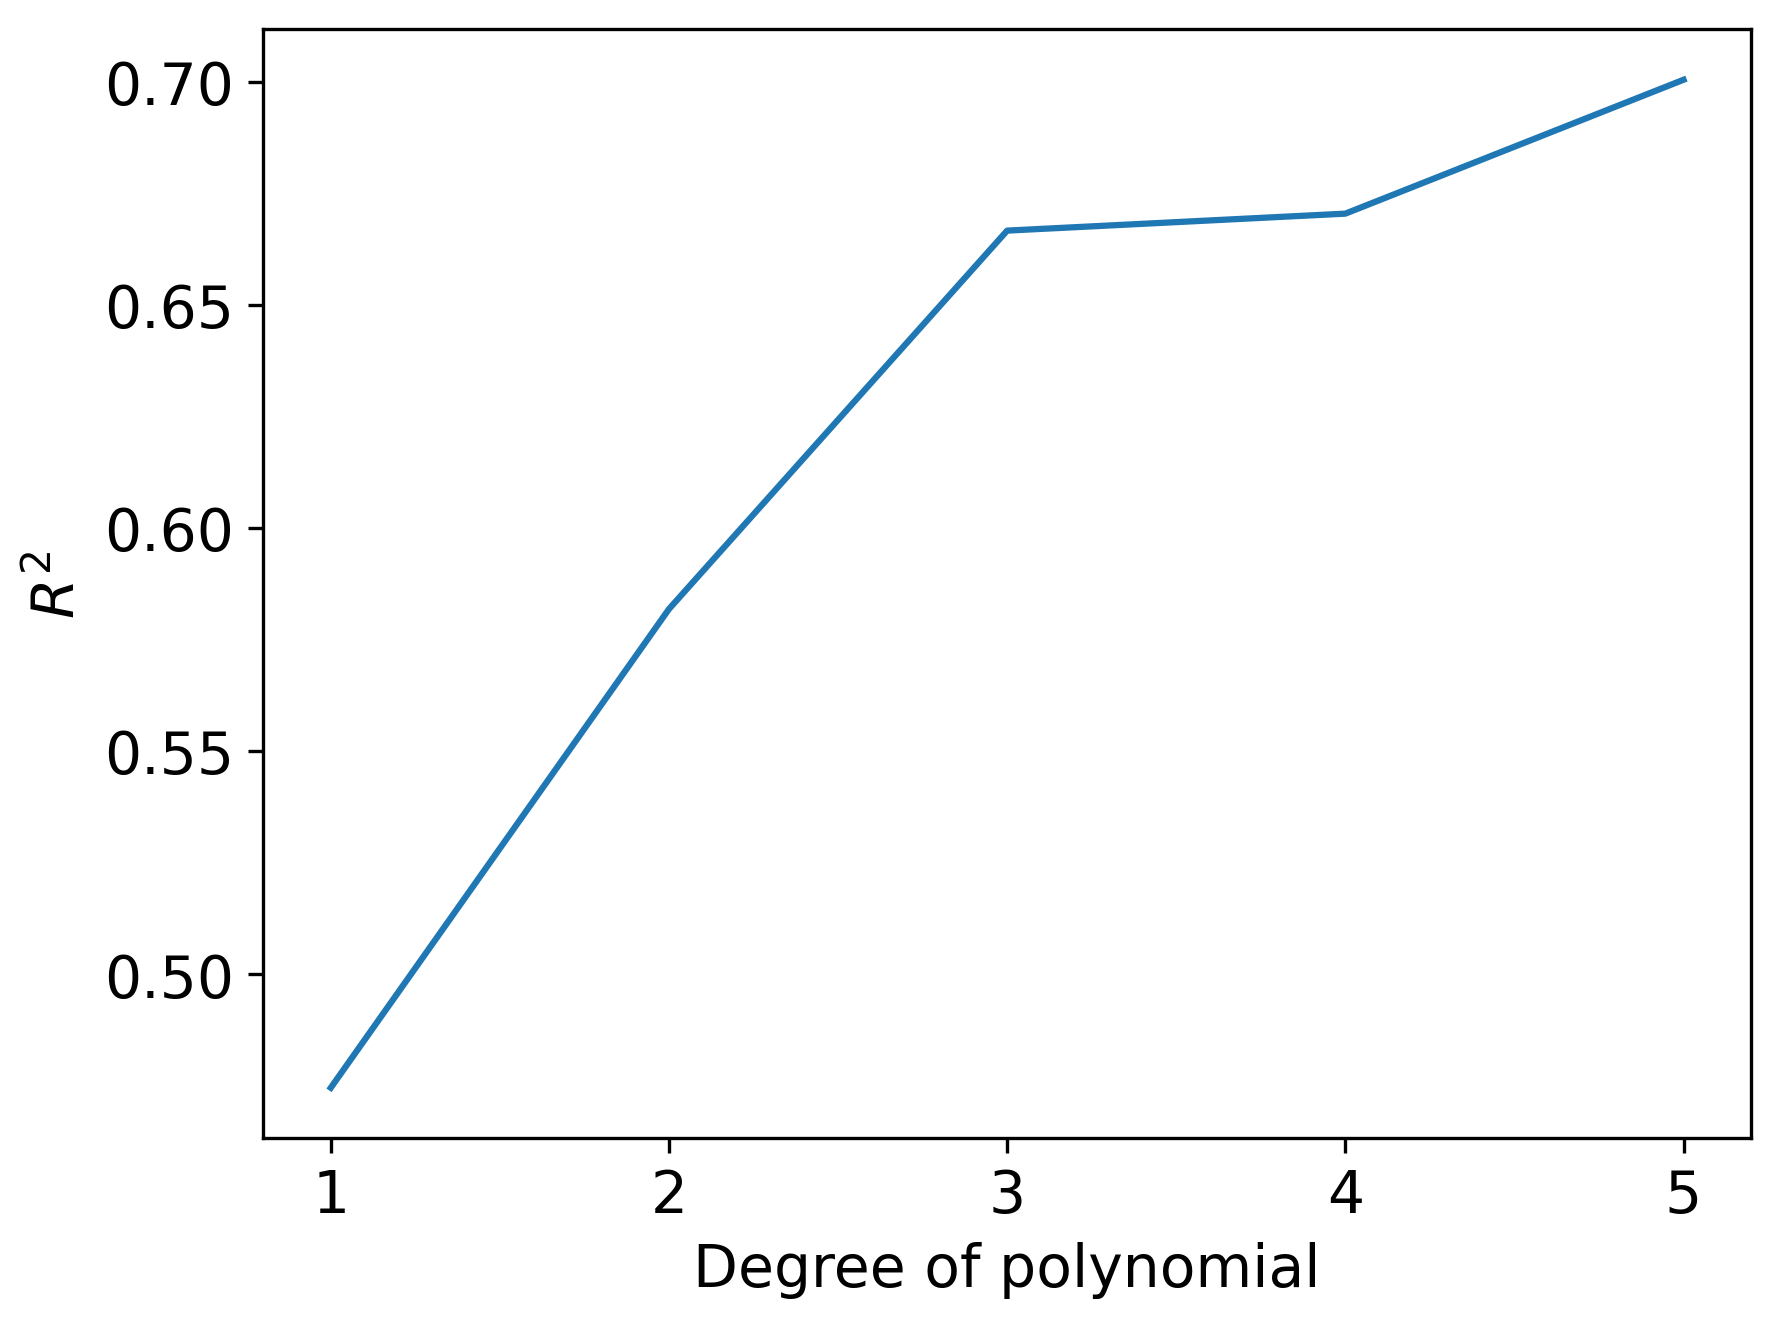
\includegraphics[width=\textwidth]{../figures/r2_ols_5.png}
    \caption{$R^2$}
    \label{fig:}
  \end{subfigure}
  \caption{plots of MSE and $R^2$ for the Franke function for an error $\epsilon \sim N(0, \sigma^2)$ with $\sigma=0.2$ and 31 points in each direction}
  \label{fig:r2_mse_5}
\end{figure}
Above in figure \ref{fig:r2_mse_5} we see a clear reduction in MSE for an increase in polynomial degree of the design matrix. For $R^2$ we see increasing values for higher degrees, with degree 5 giving us the lowest MSE and highest $R^2$ indicating degree 5 being the most optimal degree.

We continue to look into MSE and $R^2$ but now for higher degrees and also comparing the use of train or test data in the prediction of $z$. We continue using $n=30$ steps and $\sigma=0.2$. In figure \ref{fig:train_test} we see a single run and the following MSE and $R^2$ while we in figure \ref{fig:train_test_resample} see a plot of a resample of the noise data giving us 100 unique datasets to take the mean of.
\begin{figure}[H]
  \begin{subfigure}{.5\textwidth}
    \centering
    \includegraphics[width=\textwidth]{../figures/mse_train_test.png}
    \caption{$MSE$}
    \label{fig:}
  \end{subfigure}
  \begin{subfigure}{.5\textwidth}
    \centering
    \includegraphics[width=\textwidth]{../figures/r2_train_test.png}
    \caption{$R^2$}
    \label{fig:}
  \end{subfigure}
  \caption{MSE and $R^2$ computed from both the train and test sample}
  \label{fig:train_test}
\end{figure}
Above we see that both the MSE and $R^2$ from the test sample seem to start deviating from the train sample at degrees higher than 5 which indicates overfitting for greater degrees.
\begin{figure}[H]
  \begin{subfigure}{.5\textwidth}
    \centering
    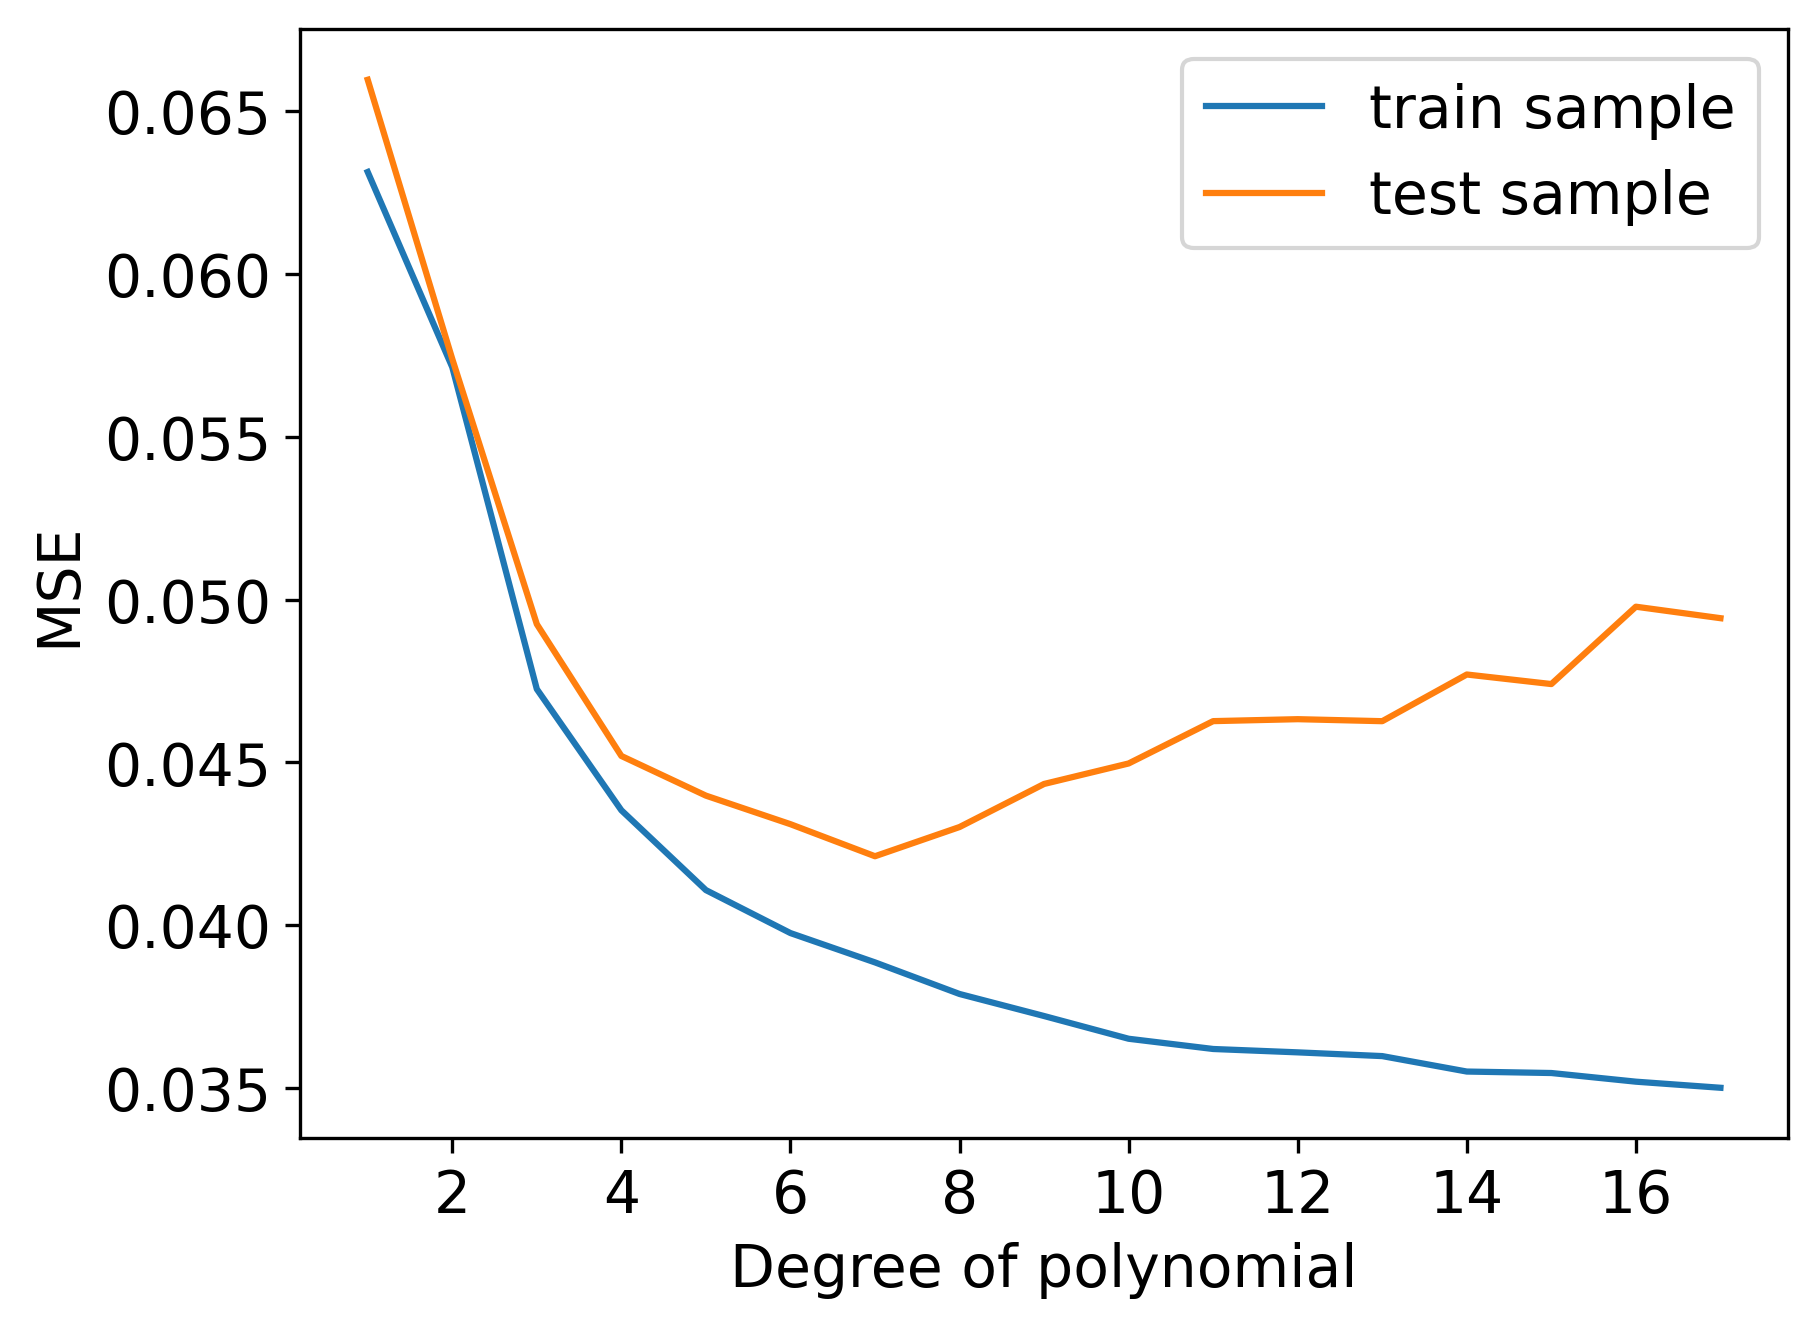
\includegraphics[width=\textwidth]{../figures/MSE_train_test_resample.png}
    \caption{$MSE$}
    \label{fig:train_test_resample_mse}
  \end{subfigure}
  \begin{subfigure}{.5\textwidth}
    \centering
    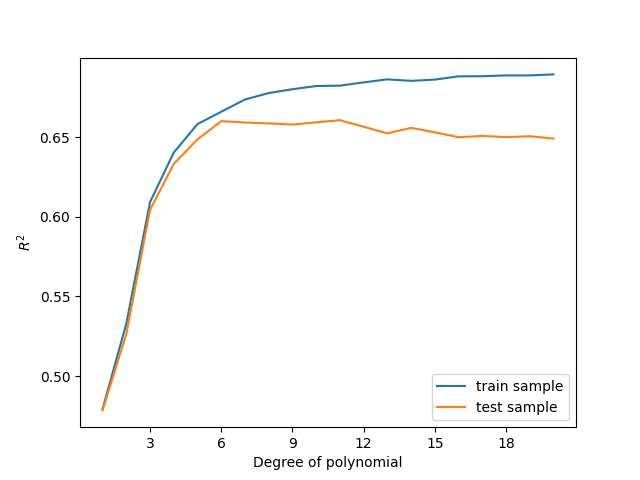
\includegraphics[width=\textwidth]{../figures/R2_train_test_resample.png}
    \caption{$R^2$}
    \label{fig:train_test_resample_r2}
  \end{subfigure}
  \caption{An average of MSE and $R^2$ computed from both the train and test sample over 100 unique samples}
  \label{fig:train_test_resample}
\end{figure}
Above in figure \ref{fig:train_test_resample} we get a smoother plot showing the smallest MSE obtained from a degree of 6 indicating this being the best polynomial degree for OLS regression of the Franke function. The $R^2$ show the same tendency but looks like having the greatest values at a degree of 8.

\subsubsection{Variation of $\beta$ parameters}

To see how the $\beta$ parameters variate from different choices of degrees we plot them for a degree up to 5 indicated in figure \ref{fig:beta} below:
\begin{figure}[H]
  \centering
  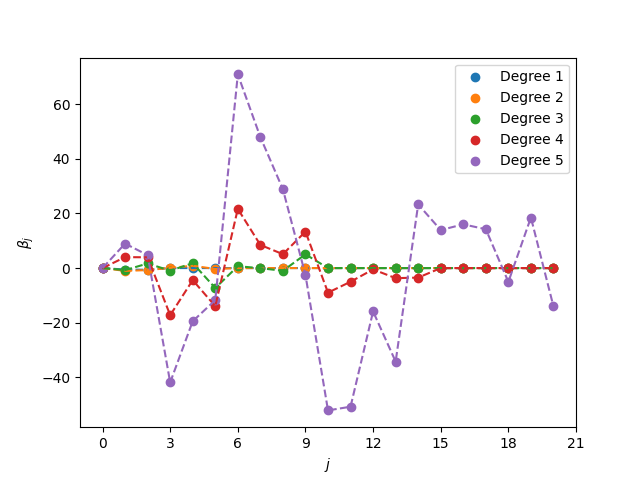
\includegraphics[width=.7\textwidth]{../figures/beta_degree.png}
  \caption{}
  \label{fig:beta}
\end{figure}
We see an increase in distance between the $\beta$ parameters for an increasing polynomial degree. When we at the same time look at table \ref{tab:beta} we see that the parameters for a degree of 5 come with great variance. This is especially true for parameters of index in the interval [6,14] which we also see in figure \ref{fig:beta} have larger values than the rest. This may be an indication of overfitting, but looking back at our resampled train test MSE plot in figure \ref{fig:train_test_resample_mse} we see that we for a degree of 5 have lower MSE than lower polynomial degrees which indicates we have still not reached overfitting.

For Ridge and Lasso regression we look into the $\beta$ parameters reaction to different choices of $\lambda$ for a polynomial degree of 5 as seen under in figure \ref{fig:beta_lambda_rl}.
\begin{figure}[H]
  \begin{subfigure}{.5\textwidth}
    \centering
    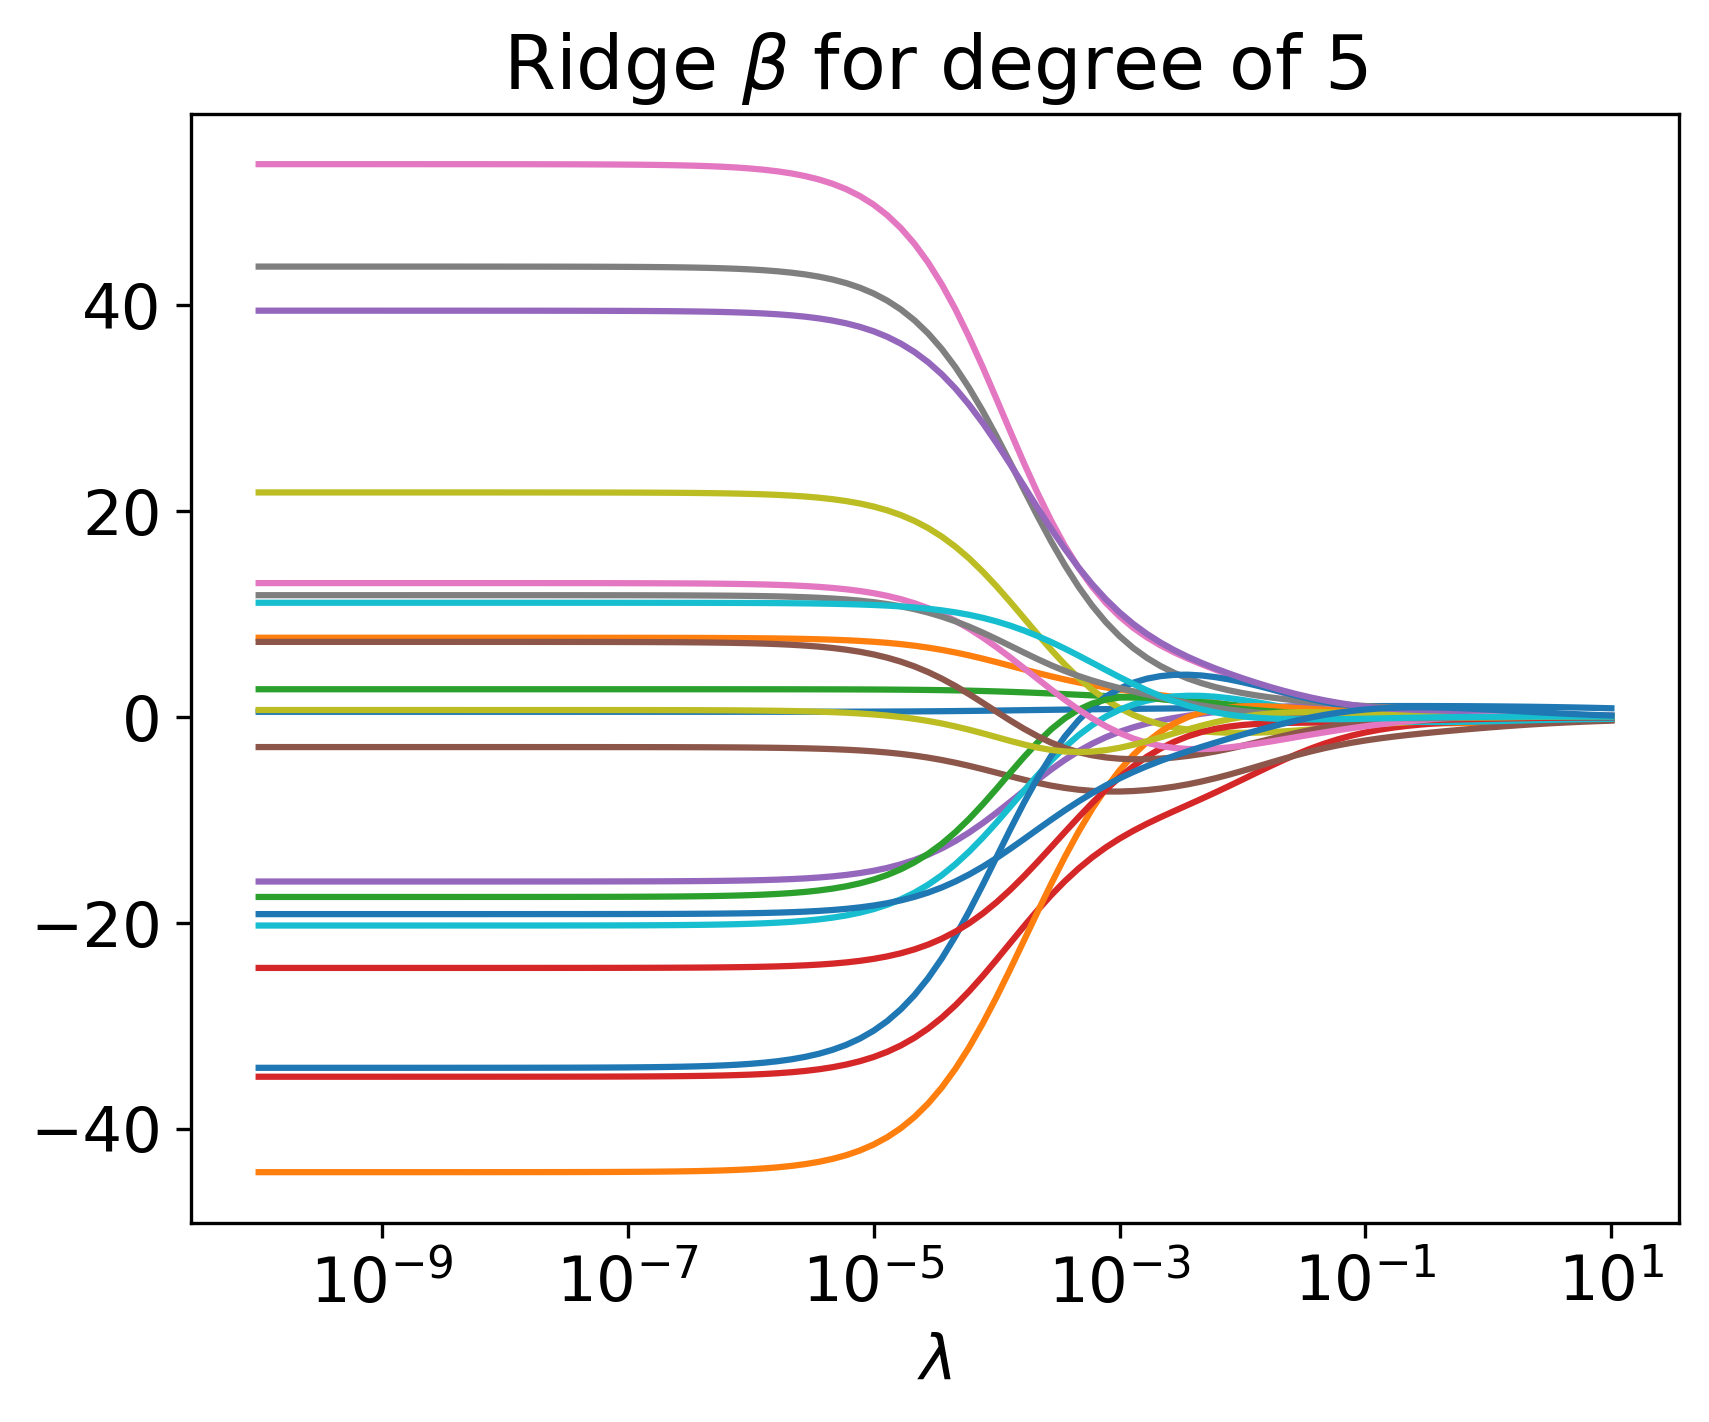
\includegraphics[width=\textwidth]{../figures/ridge_beta.png}
    \caption{Ridge}
    \label{fig:}
  \end{subfigure}
  \begin{subfigure}{.5\textwidth}
    \centering
    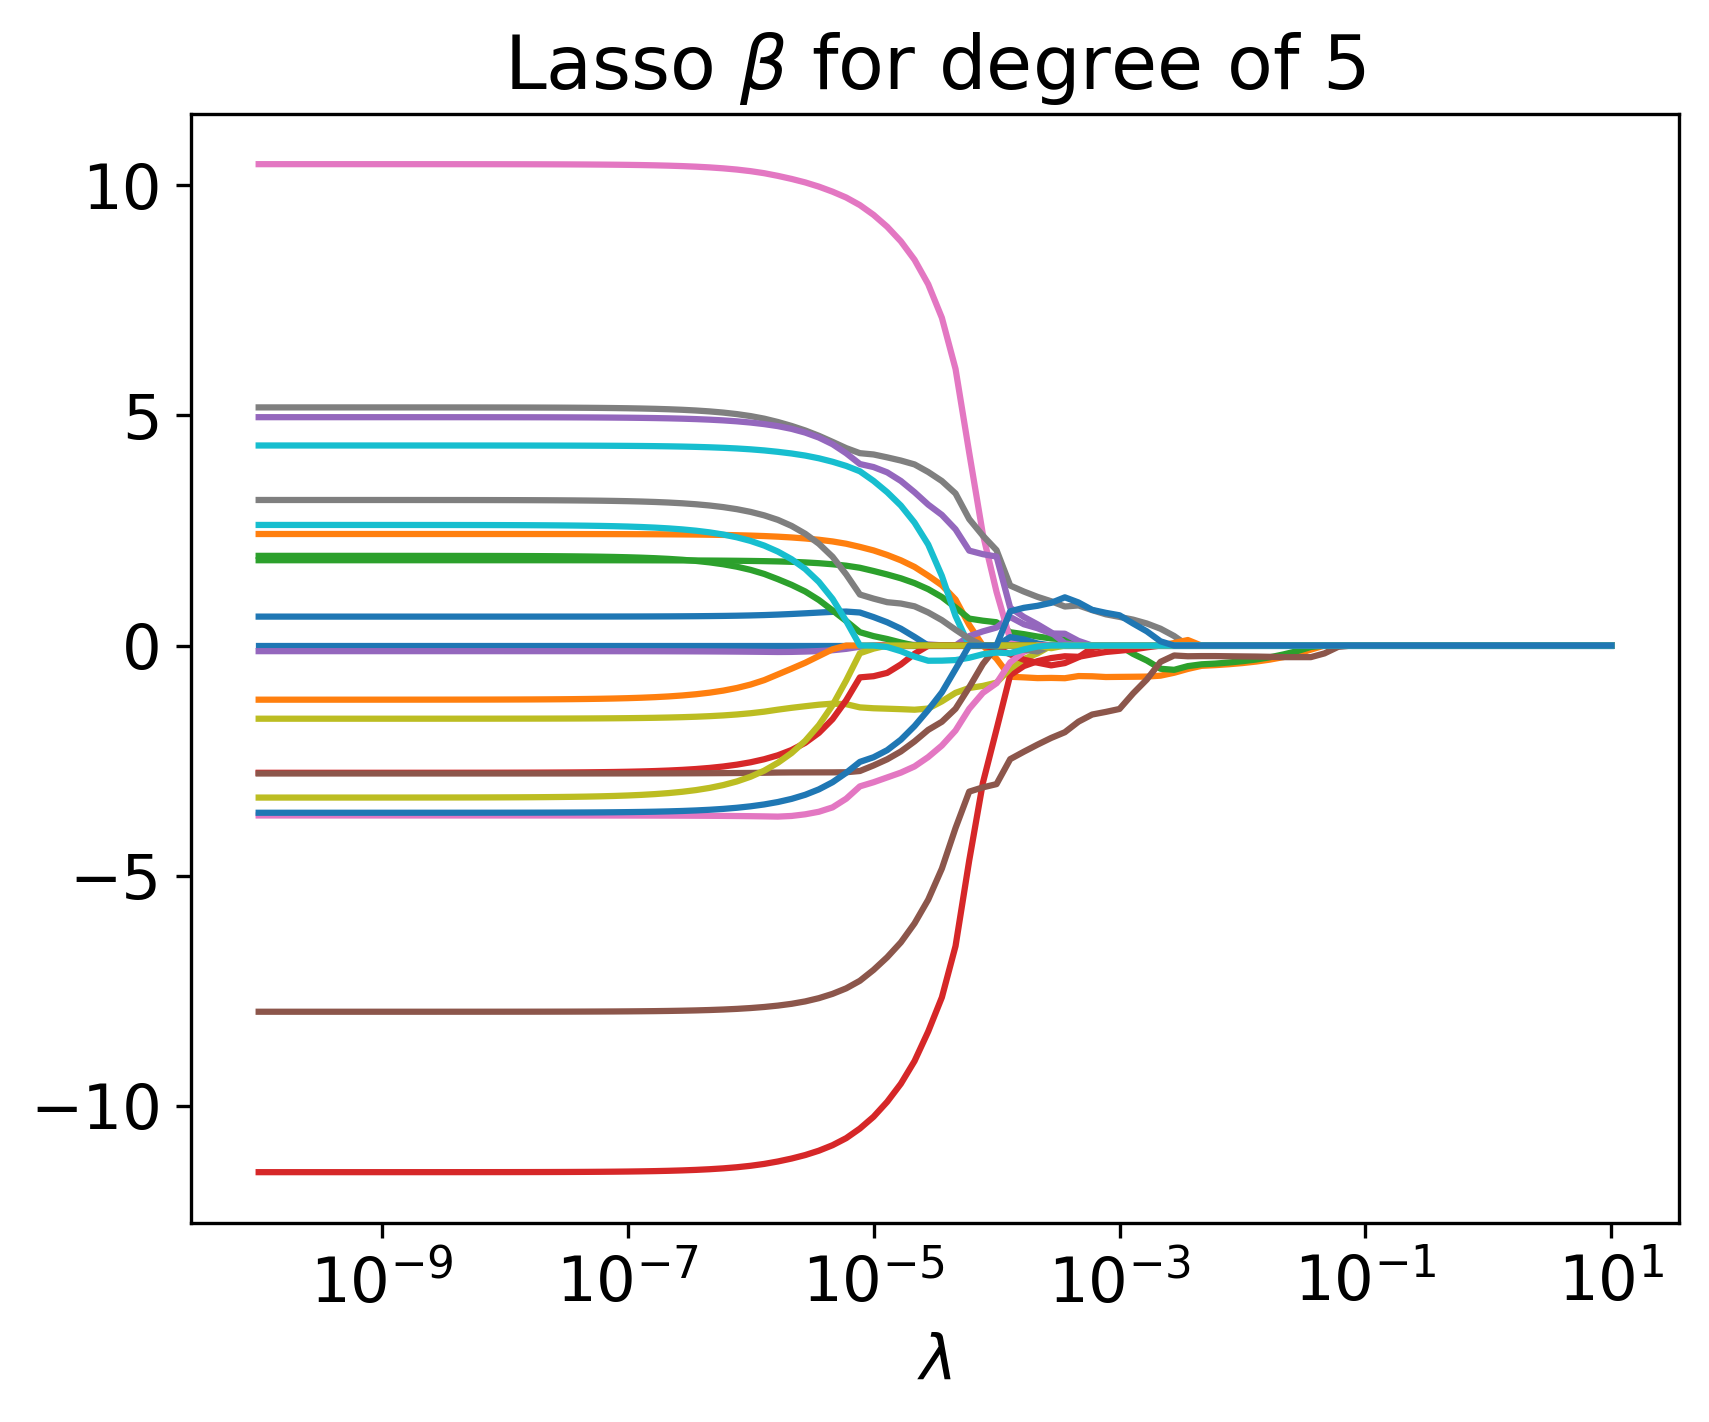
\includegraphics[width=\textwidth]{../figures/lasso_beta.png}
    \caption{Lasso}
    \label{fig:}
  \end{subfigure}
  \caption{A comparison on how $\lambda$ influences the $\beta$ values between Ridge and Lasso regression}
  \label{fig:beta_lambda_rl}
\end{figure}
We see a clear correlation between the magnitude of $\beta$ and the size of $\lambda$. We can also see that Lasso more quickly reduces $\beta$ to 0 while Ridge seems to allow larger values of $\beta$ exist for larger values of $\lambda$. We also see that the beta parameters looks to have same values as we saw for OLS in figure \ref{fig:beta} for smaller values of $\lambda$

\begin{table}[H]
  \caption{Variance of the $\beta$ parameters for test and train data for a design matrix of polynomial degree 5. Calculated by $Var(\boldsymbol{\beta}) = diag(\sigma^2(X^T X)^{-1}$)}
  \label{tab:beta}
  \centering
  \begin{tabular}{|c|c|c|}
    \hline
    $\boldsymbol{\beta}$ &\textbf{Test data} & \textbf{Train data} \\\hline
    $\beta_{0}$ & 0.04 & 0.01 \\
    $\beta_{1}$ & 5.22 & 1.31 \\
    $\beta_{2}$ & 6.00 & 1.27 \\
    $\beta_{3}$ & 139.88 & 31.56 \\
    $\beta_{4}$ & 90.01 & 19.04 \\
    $\beta_{5}$ & 149.50 & 31.37 \\
    $\beta_{6}$ & 723.58 & 162.55 \\
    $\beta_{7}$ & 364.34 & 90.68 \\
    $\beta_{8}$ & 555.61 & 83.97 \\
    $\beta_{9}$ & 787.29 & 163.88 \\
    $\beta_{10}$ & 794.84 & 179.33 \\
    $\beta_{11}$ & 521.51 & 104.67 \\
    $\beta_{12}$ & 424.30 & 88.62 \\
    $\beta_{13}$ & 625.04 & 98.00 \\
    $\beta_{14}$ & 880.18 & 180.91 \\
    $\beta_{15}$ & 122.43 & 27.74 \\
    $\beta_{16}$ & 102.30 & 20.80 \\
    $\beta_{17}$ & 80.15 & 19.80 \\
    $\beta_{18}$ & 108.00 & 19.14 \\
    $\beta_{19}$ & 105.44 & 20.14 \\
    $\beta_{20}$ & 134.90 & 27.84 \\
    \hline
  \end{tabular}
\end{table}

\subsubsection{The bias variance tradeoff}

To further analyze our models dependence on polynomial degree we have a plot of the bias variance tradeoff in figure \ref{fig:bias_variance} for a degree up to 15 using $n=30$ steps and a noise standard deviation of $\sigma=0.2$.
\begin{figure}[H]
  \centering
  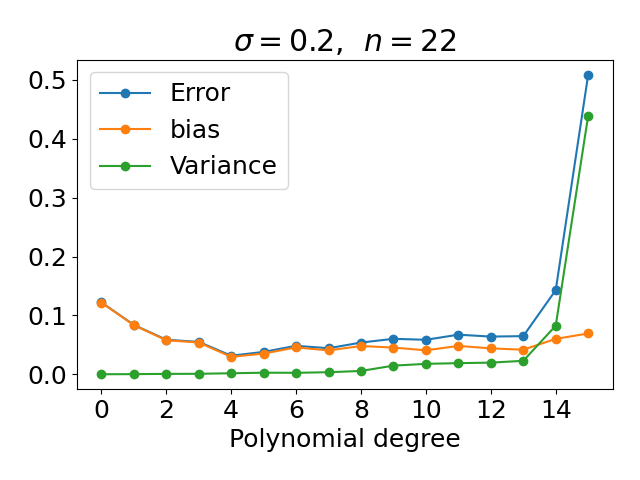
\includegraphics[width=\textwidth]{../figures/bias_variance_tradeoff.png}
  \caption{The bias variance tradeoff for the Franke function using 100 bootstrap iteration together with $n=30$ steps and a noise standard deviation of $\sigma=0.2$}
  \label{fig:bias_variance}
\end{figure}
We see above in figure \ref{fig:bias_variance} areas of both high variance and low bias and low variance and relative high bias. We also see that the area of lowest MSE for a degree of 6 is where both the bias and variance together is at their lowest. A further increase in polynomial degree gives mostly a variance dominated error contribution while we at lower polynomial degrees see that the bias is what contributes the most to the error.

When we look at figure \ref{fig:bias_variance_100} we see another trend especially for higher polynomial degrees. Here the variance stays low which may together with the low mse indicate that we do not as easily overfit our data when we have more of it at hand.
\begin{figure}[H]
  \centering
  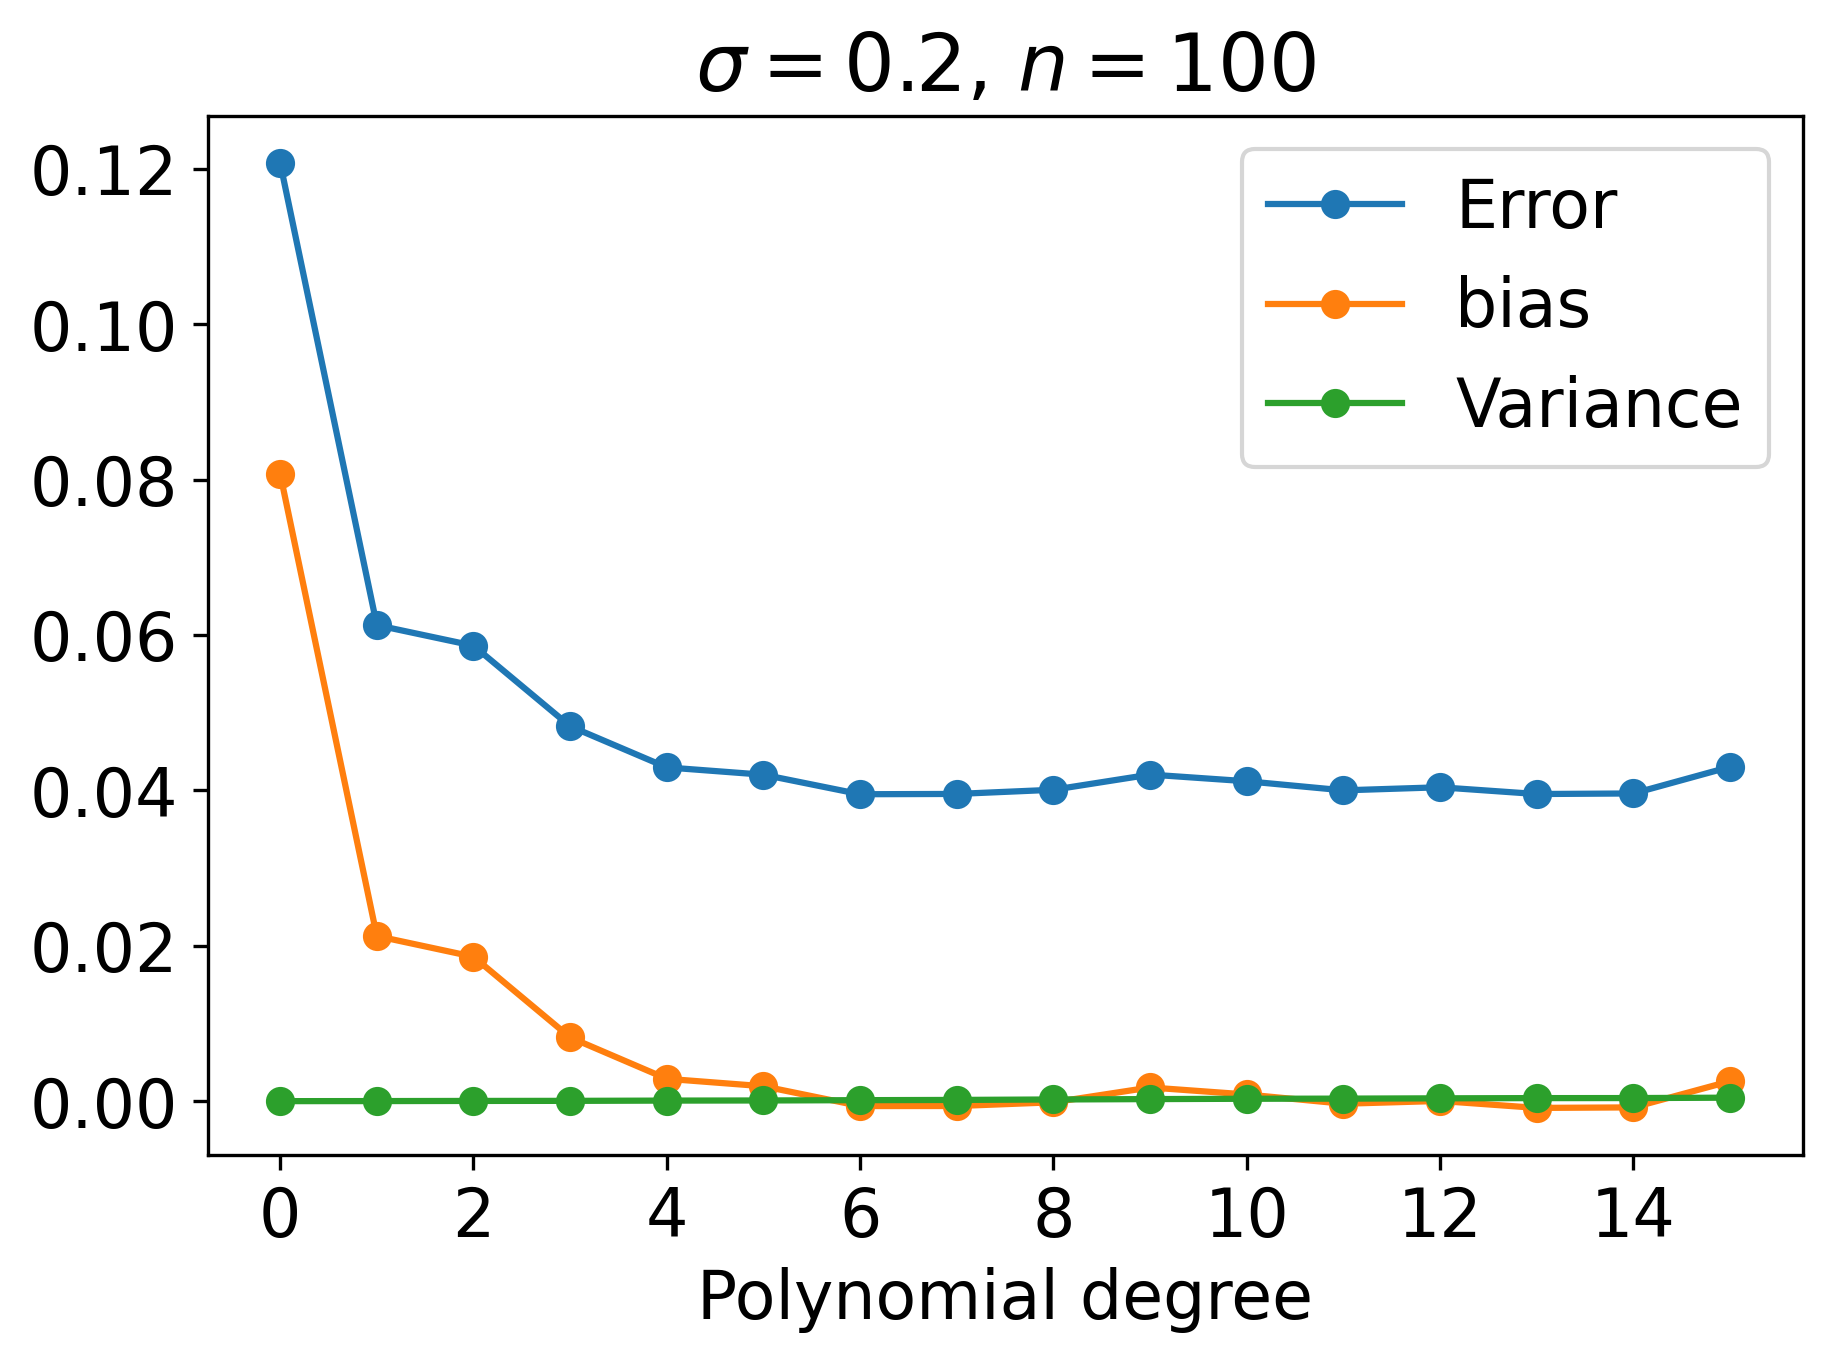
\includegraphics[width=\textwidth]{../figures/bias_variance_100.png}
  \caption{The bias variance tradeoff for the Franke function using 100 bootstrap iteration together with $n=100$ steps and a noise standard deviation of $\sigma=0.2$}
  \label{fig:bias_variance_100}
\end{figure}


In the same way as for ordinary least squares we look at the bias variance tradeoff for Ridge and Lasso, only that we now have another parameter $\lambda$ that influences the tradeoff. Under in figure \ref{fig:ridge_tradeoff} and figure \ref{fig:lasso_tradeoff} we see the tradeoff for different choices of $\lambda$ for both Ridge and Lasso regression. Here it is worth to notice when comparing to the OLS tradeoff in figure \ref{fig:bias_variance} that we for Ridge and Lasso plot for degrees up to and including 20.
\begin{figure}[H]
  \begin{subfigure}{.5\textwidth}
    \centering
    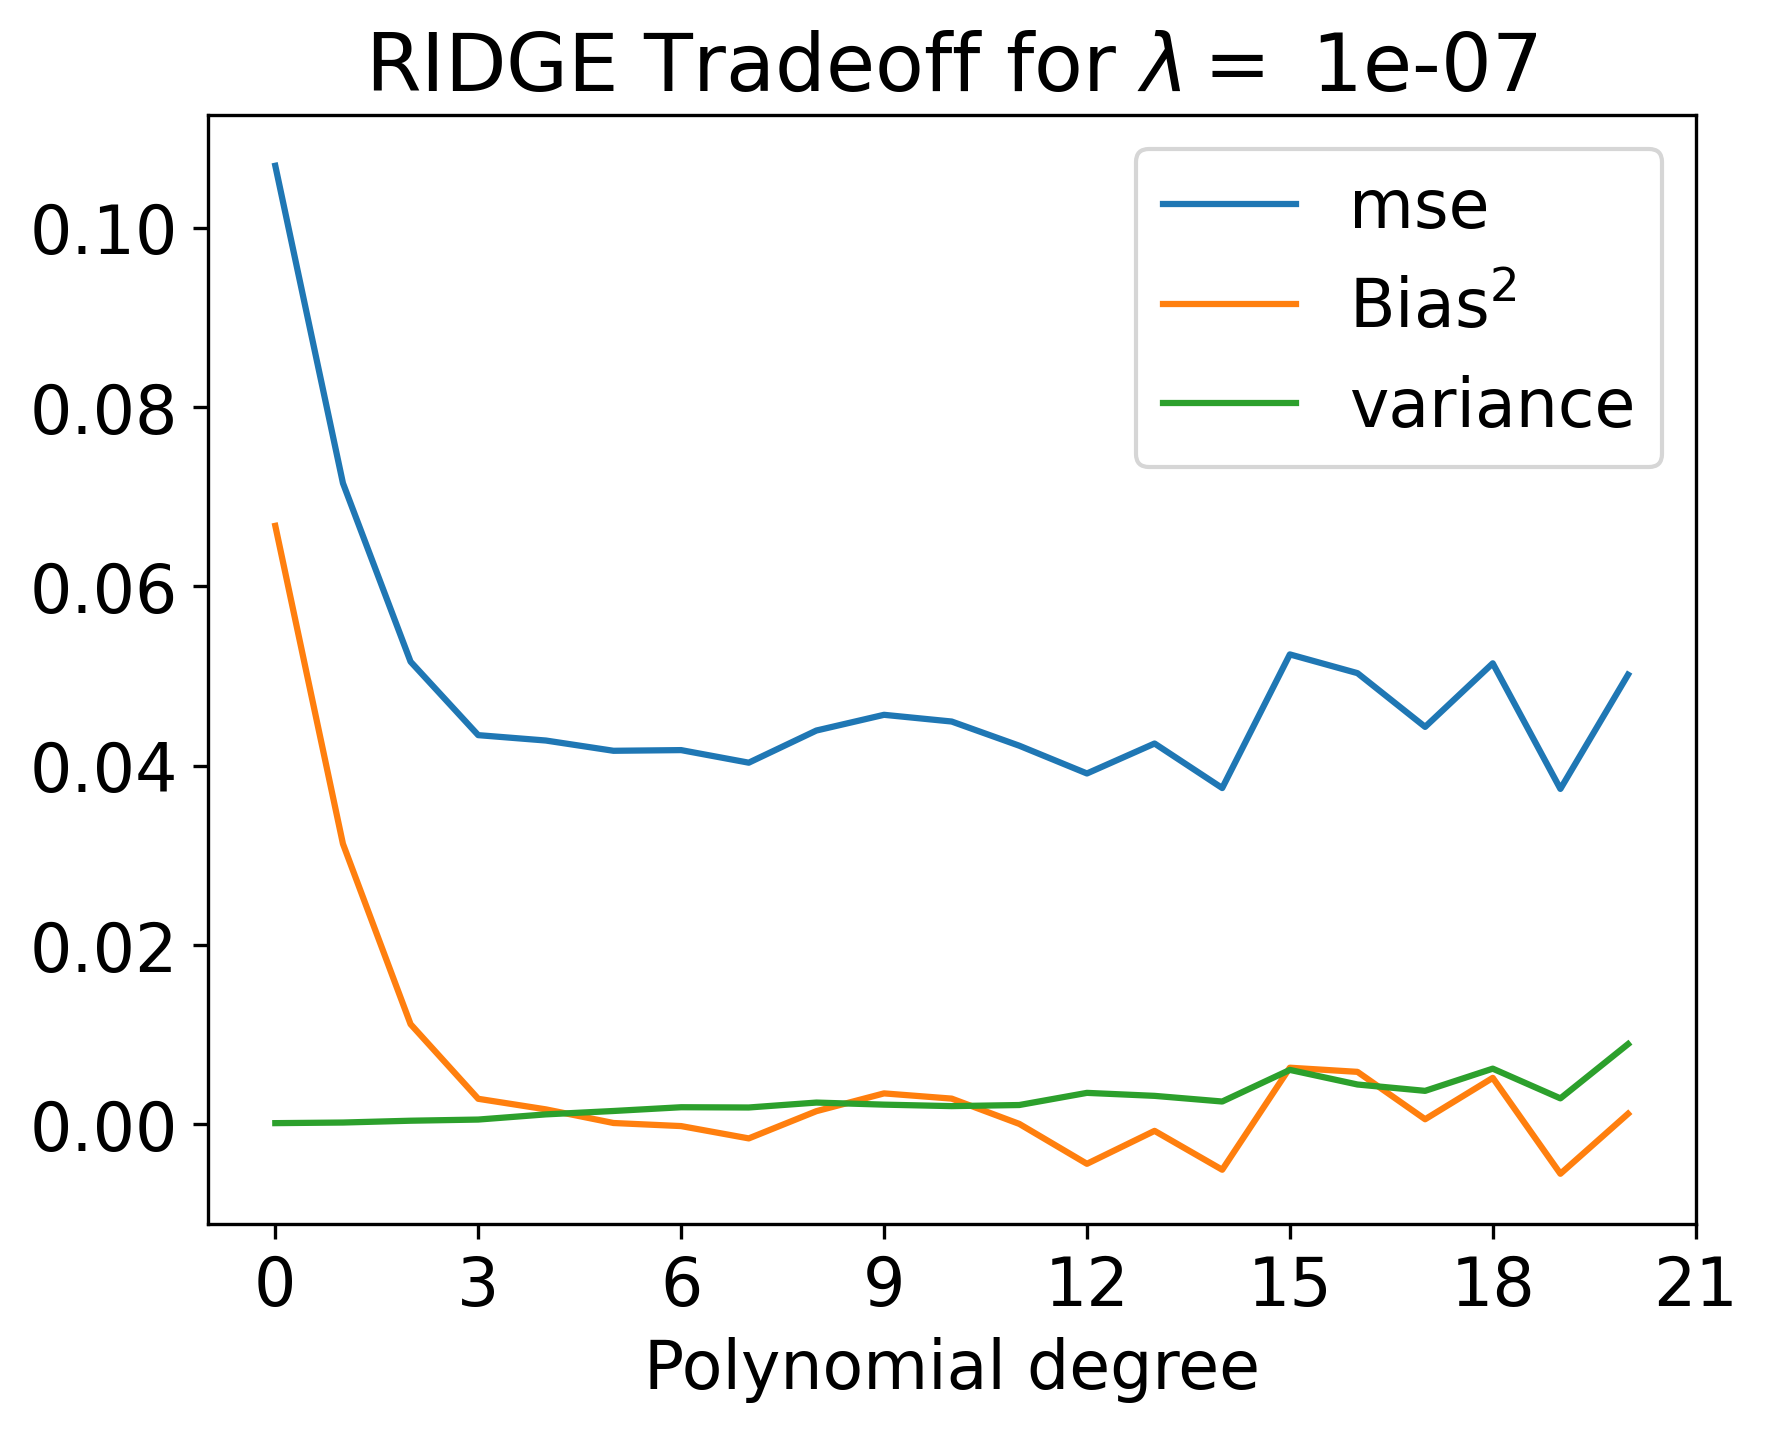
\includegraphics[width=\textwidth]{../figures/tradeoff_RIDGE_1e-07_20.png}
    \caption{}
    \label{fig:l_1e-07}
  \end{subfigure}
  \begin{subfigure}{.5\textwidth}
    \centering
    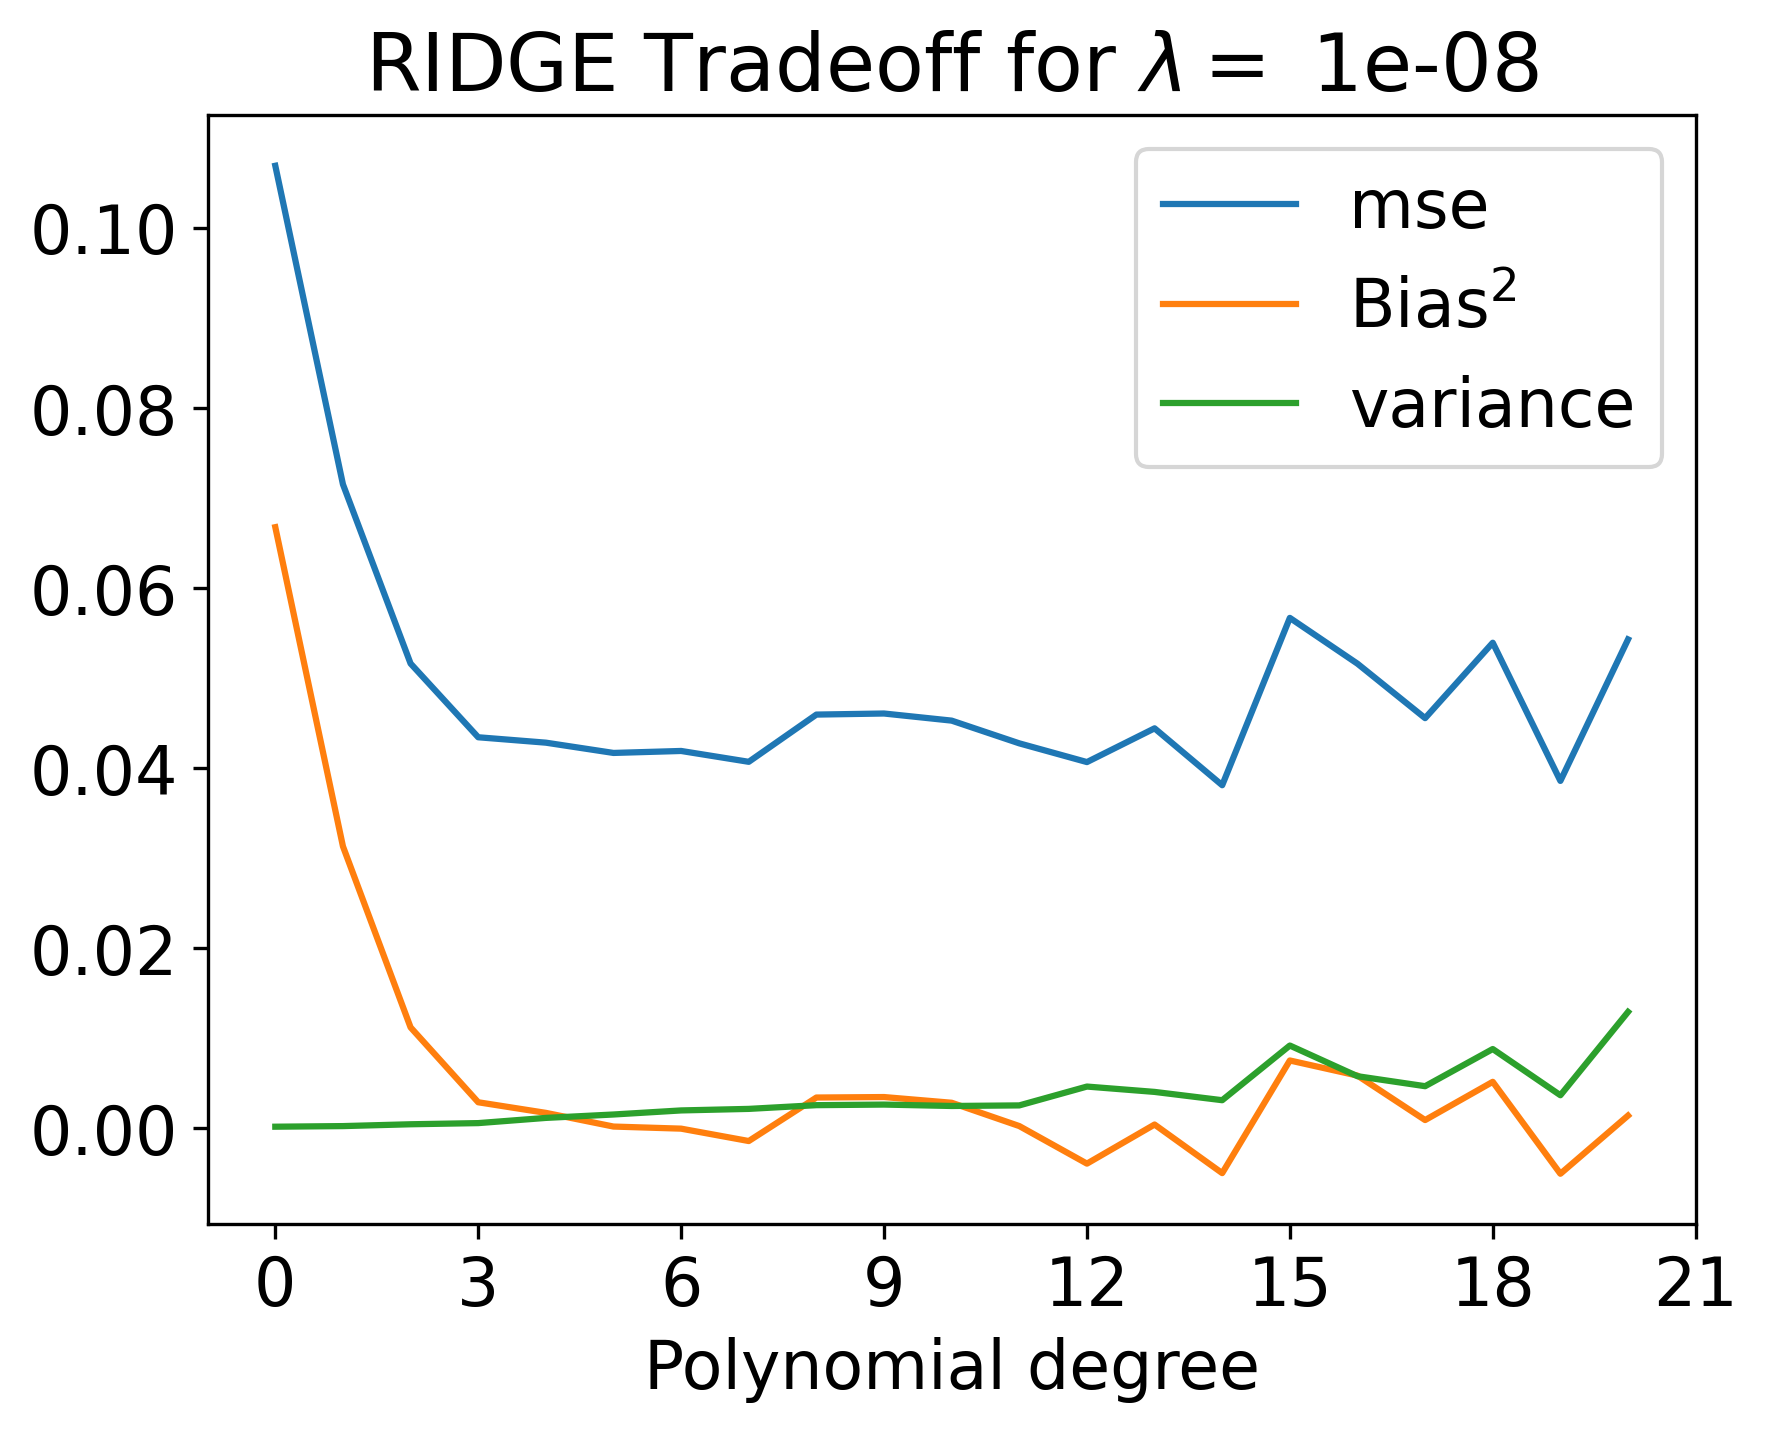
\includegraphics[width=\textwidth]{../figures/tradeoff_RIDGE_1e-08_20.png}
    \caption{}
    \label{fig:l_1e-08}
  \end{subfigure}
  \begin{subfigure}{.5\textwidth}
    \centering
    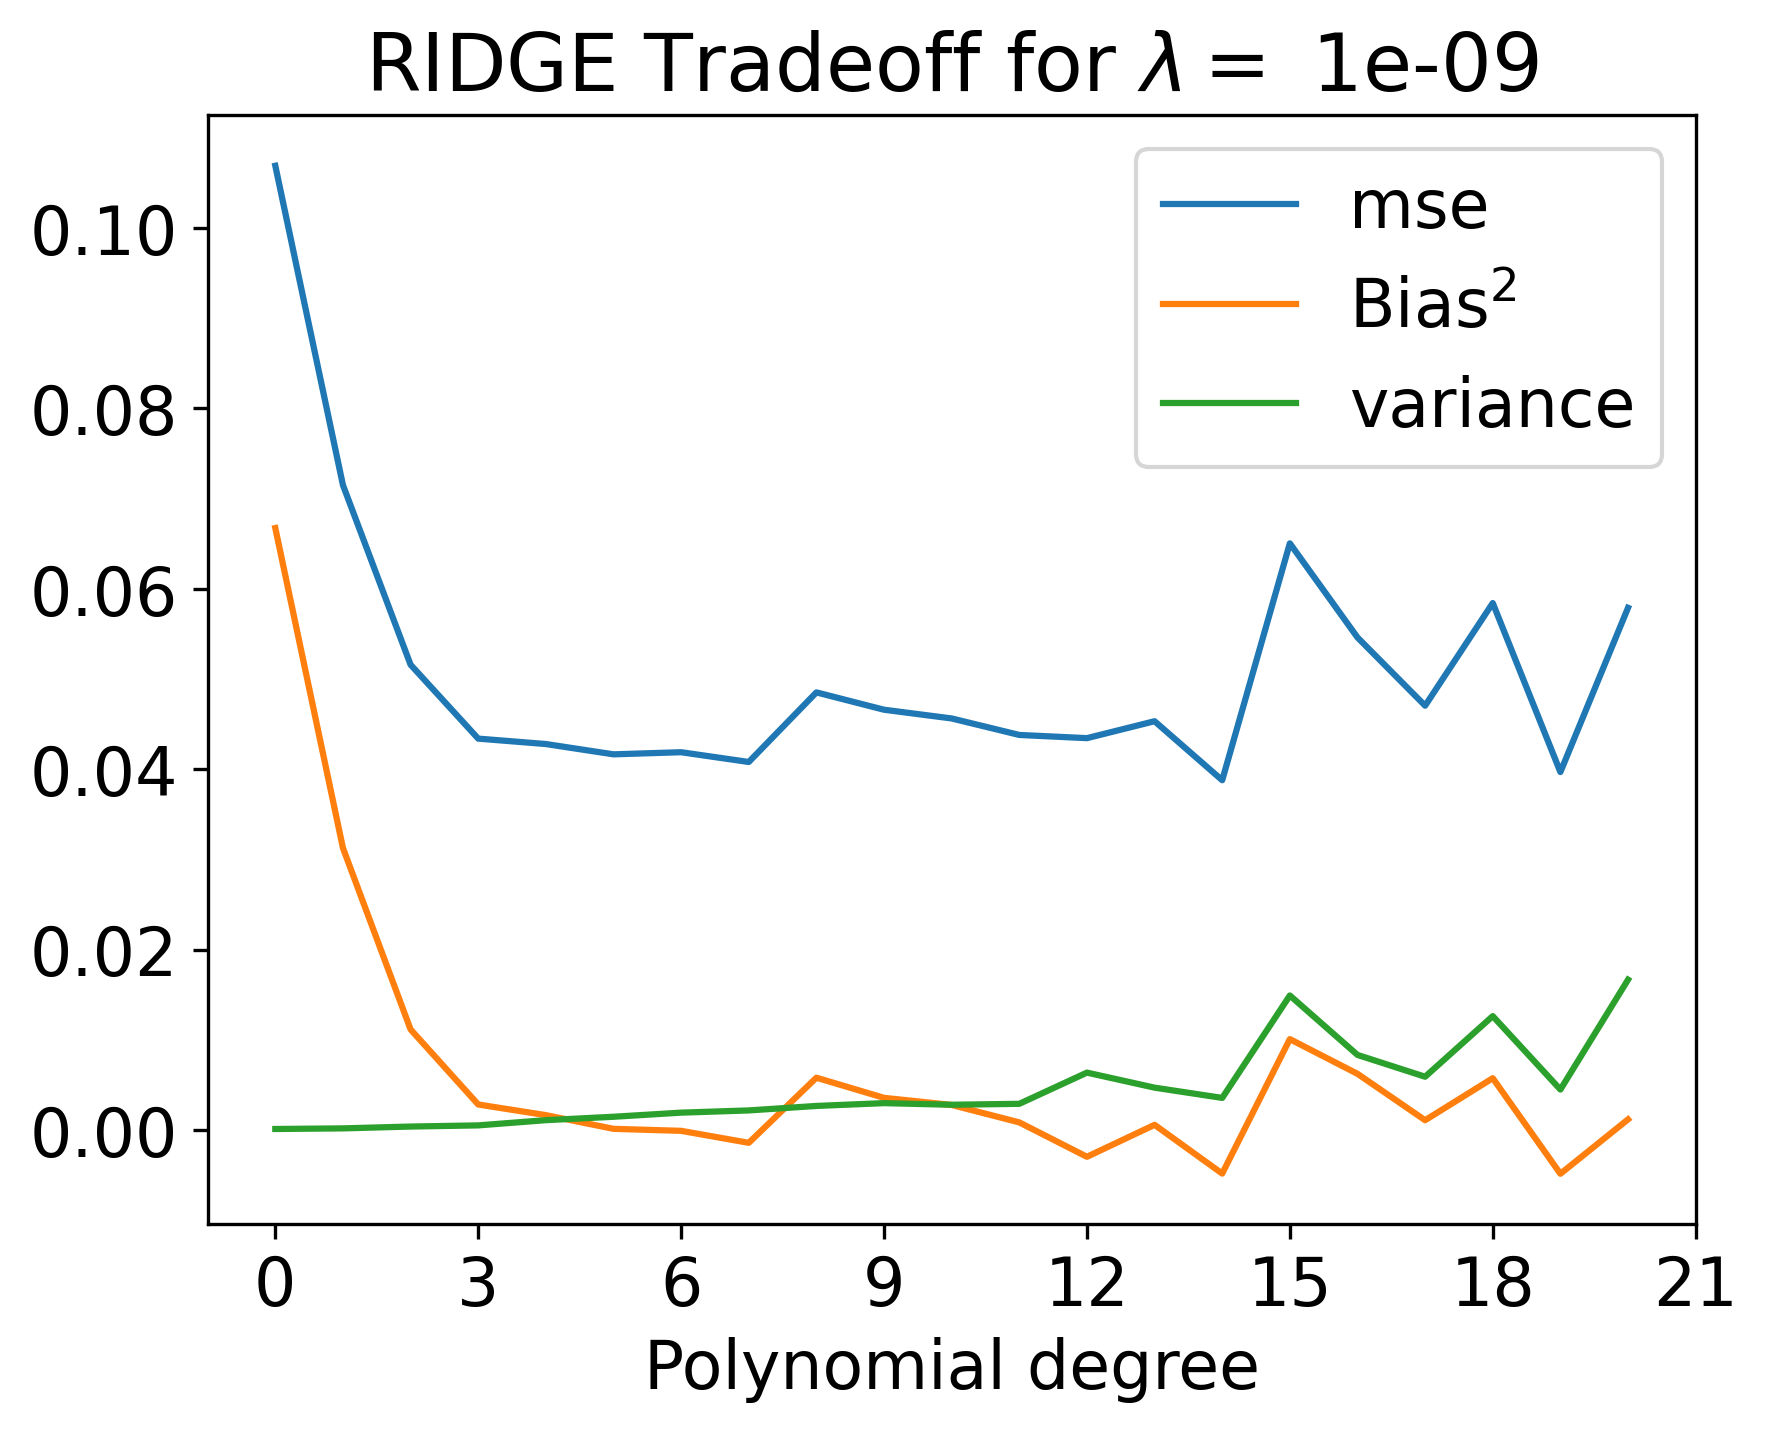
\includegraphics[width=\textwidth]{../figures/tradeoff_RIDGE_1e-09_20.png}
    \caption{}
    \label{fig:l_1e-09}
  \end{subfigure}
  \begin{subfigure}{.5\textwidth}
    \centering
    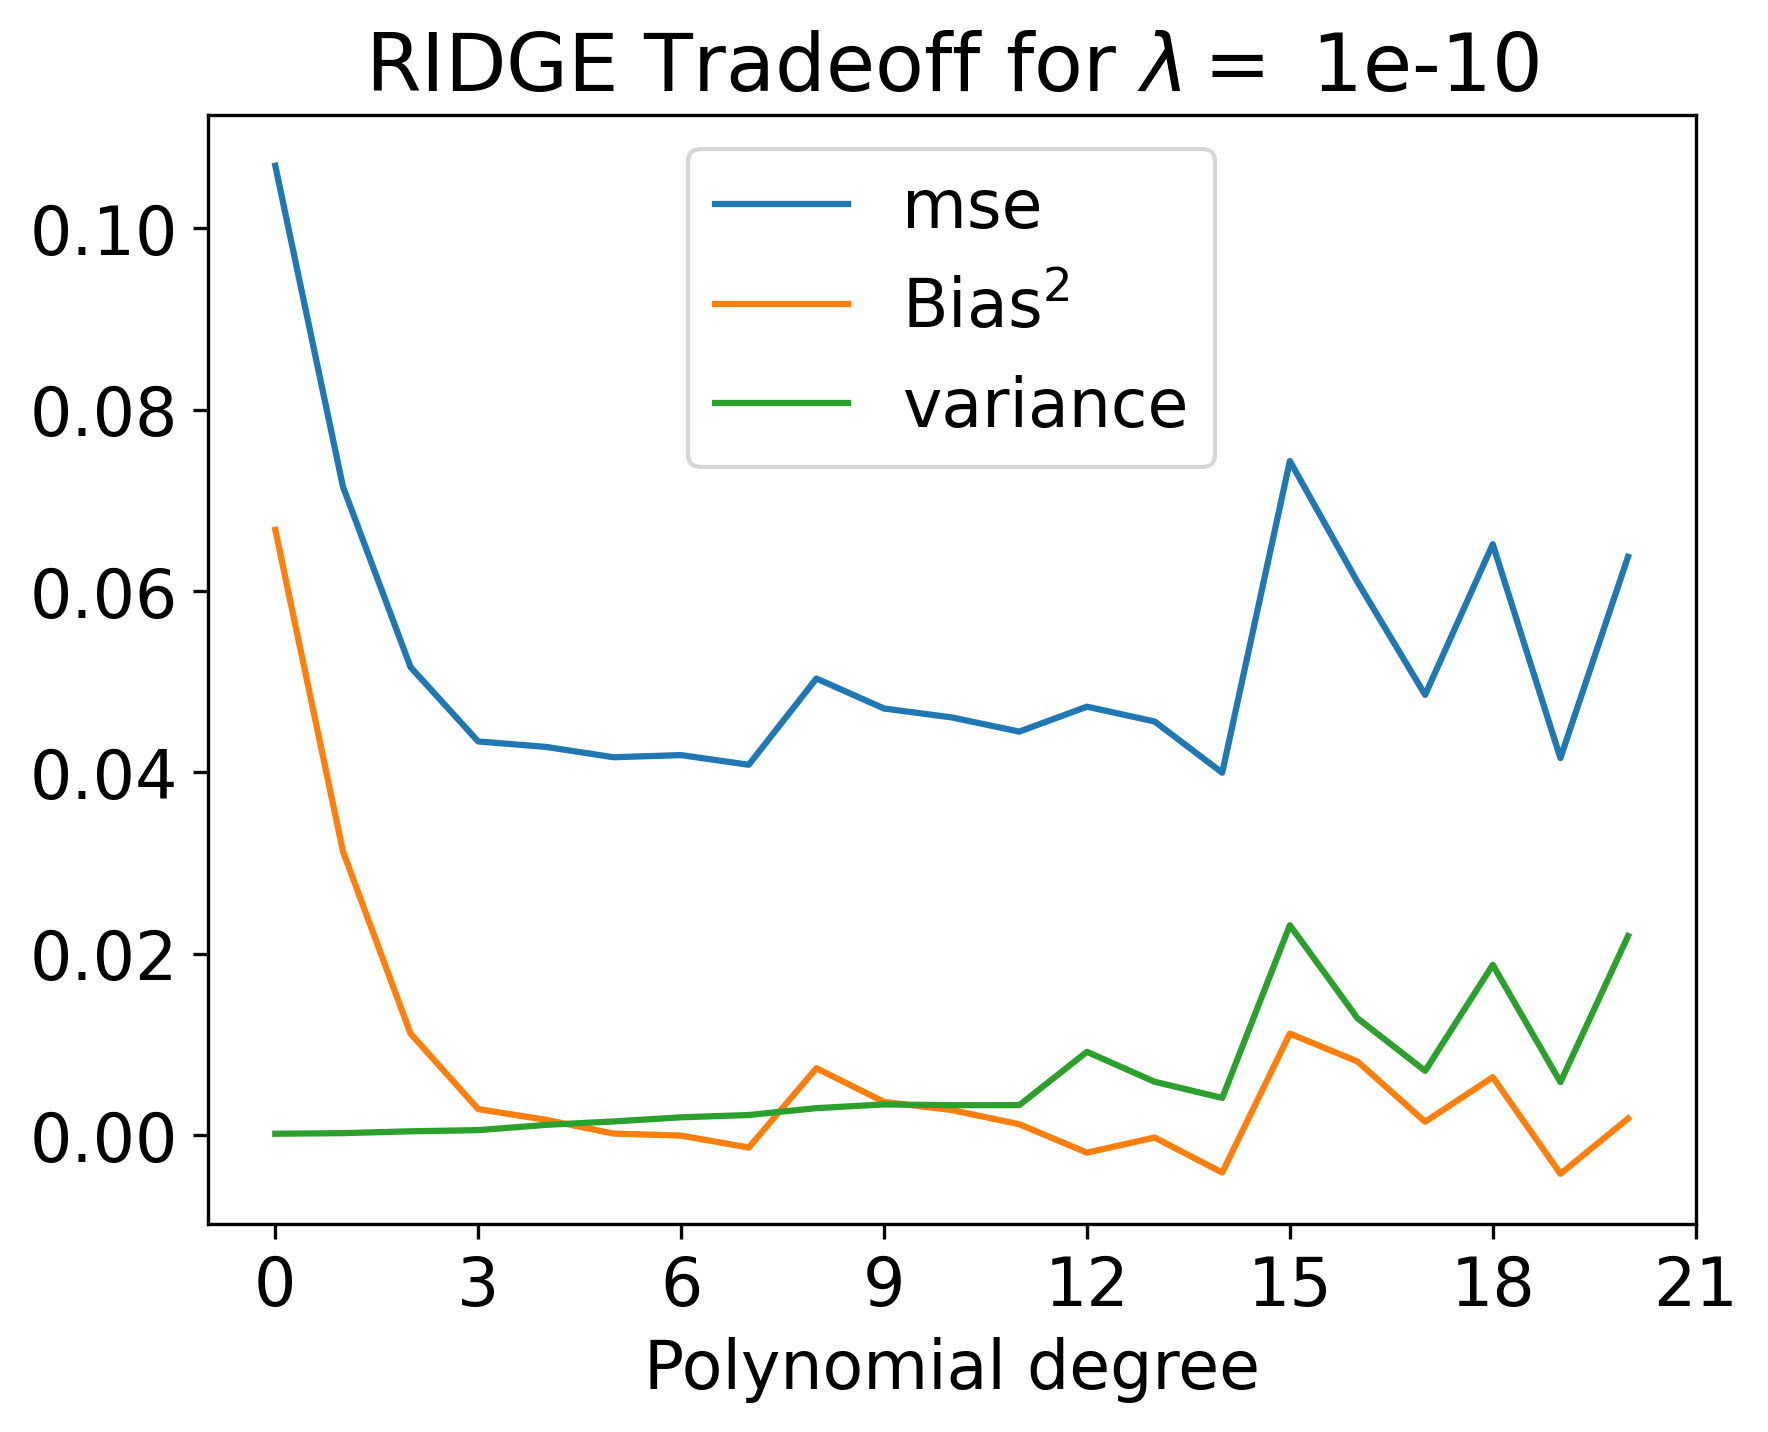
\includegraphics[width=\textwidth]{../figures/tradeoff_RIDGE_1e-10_20.png}
    \caption{}
    \label{fig:l_1e-10}
  \end{subfigure}
  \begin{subfigure}{.5\textwidth}
    \centering
    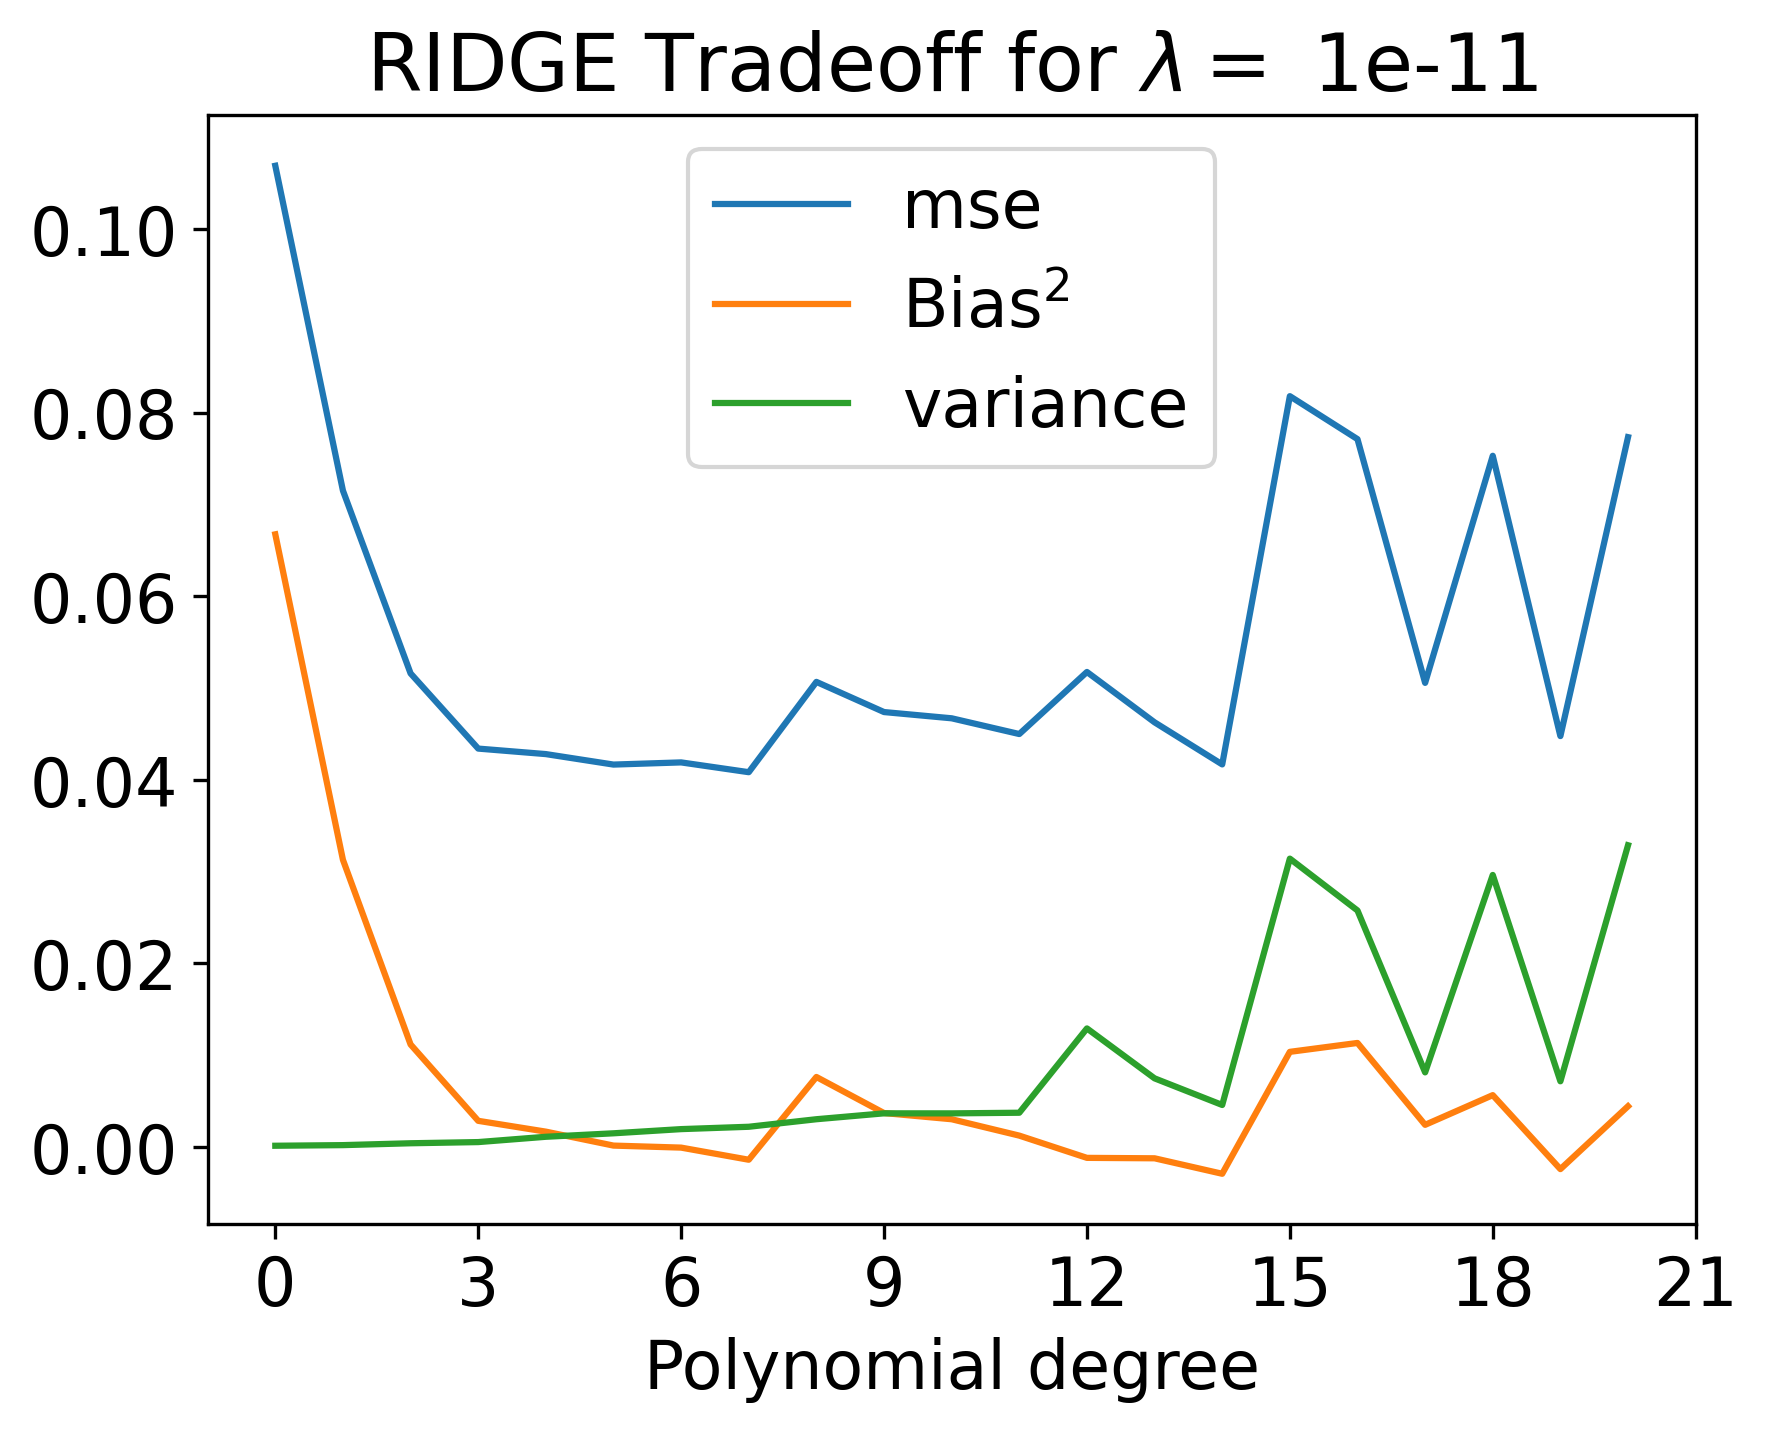
\includegraphics[width=\textwidth]{../figures/tradeoff_RIDGE_1e-11_20.png}
    \caption{}
    \label{fig:l_1e-11}
  \end{subfigure}
  \begin{subfigure}{.5\textwidth}
    \centering
    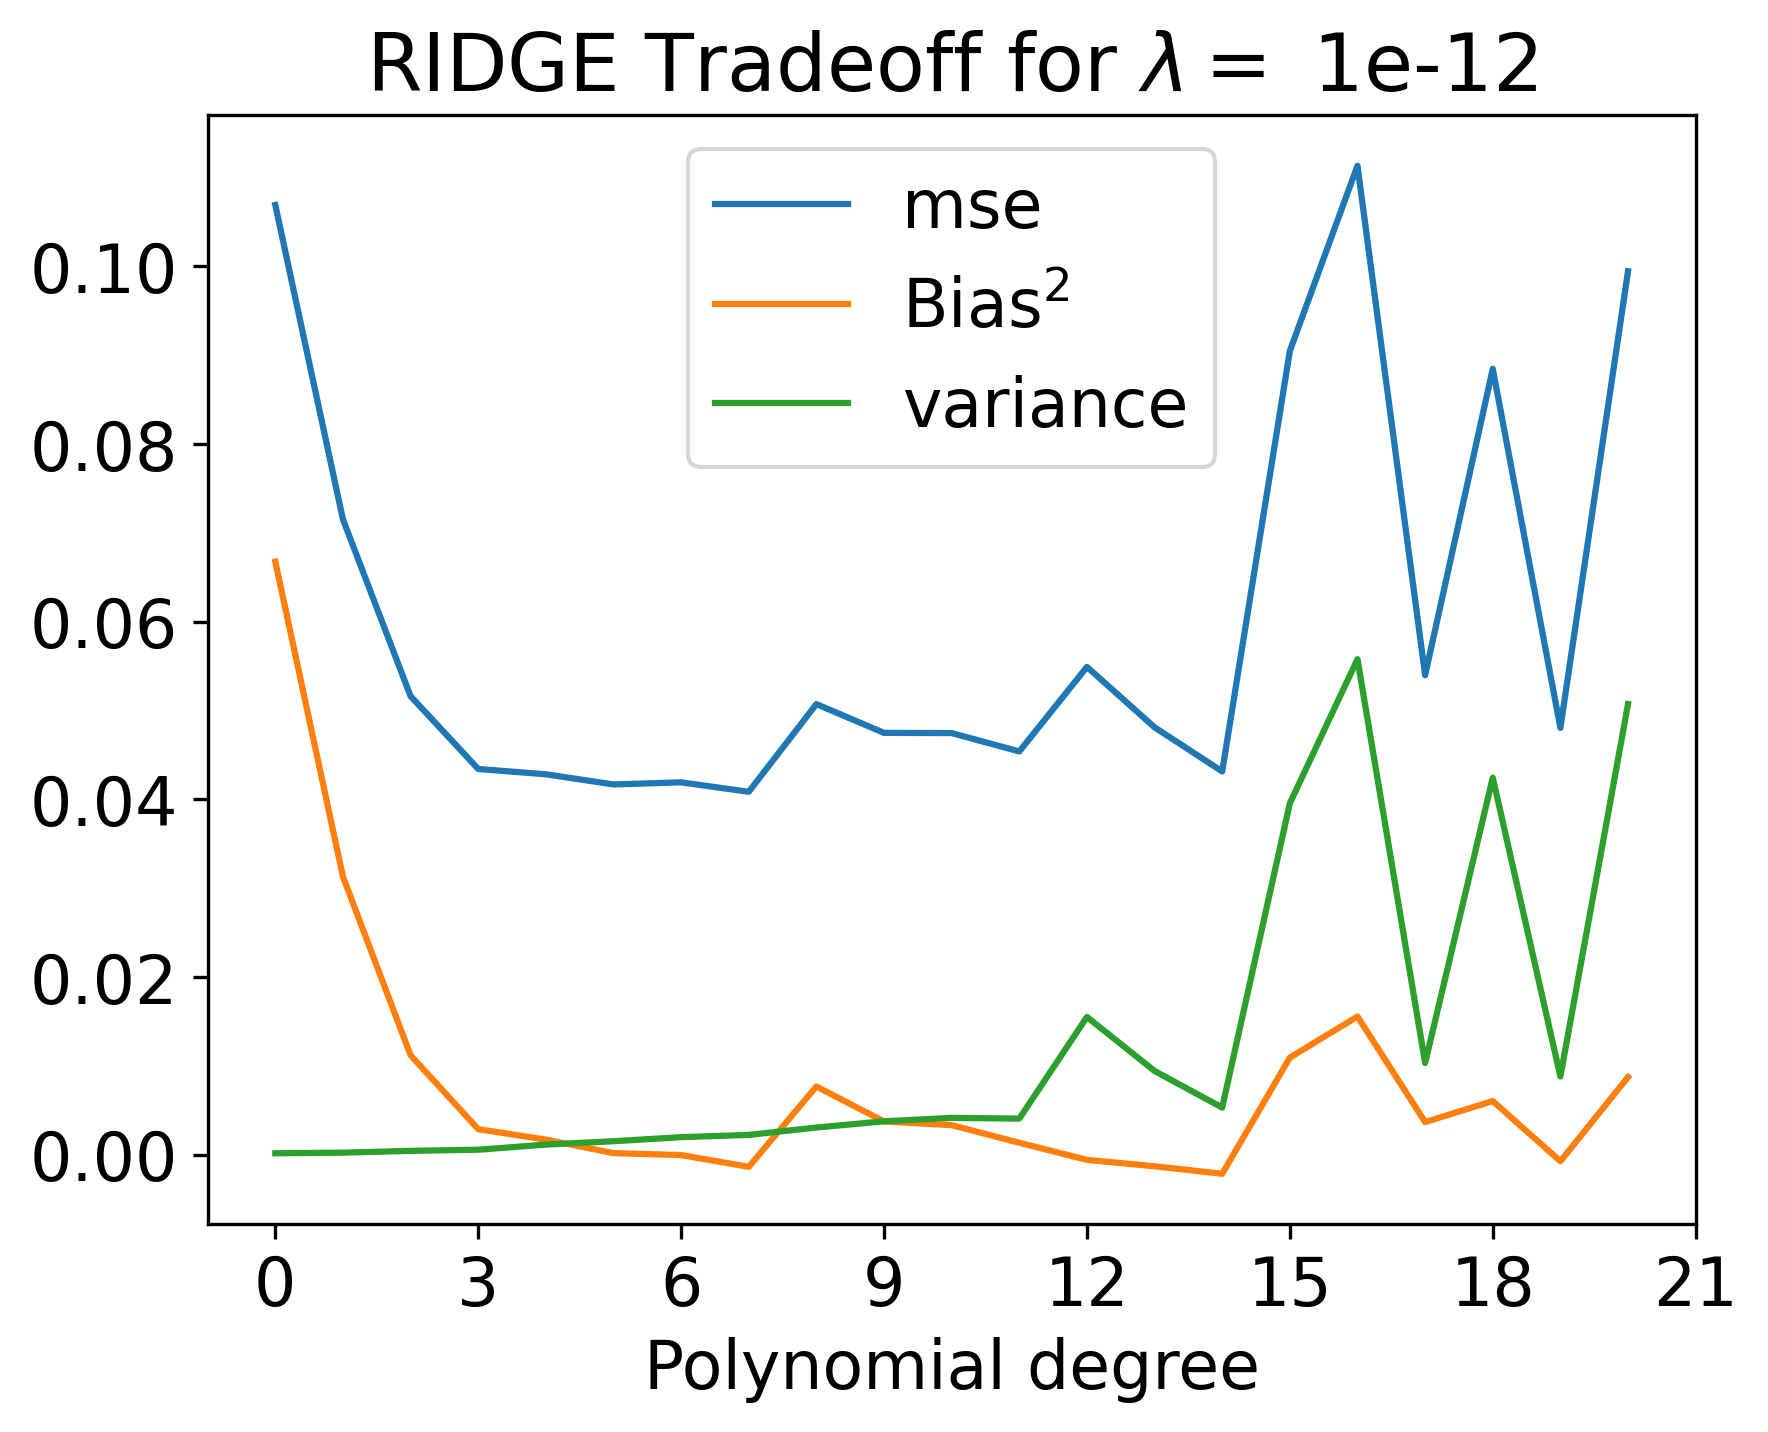
\includegraphics[width=\textwidth]{../figures/tradeoff_RIDGE_1e-12_20.png}
    \caption{}
    \label{fig:l_1e-12}
  \end{subfigure}
  \caption{Bias-variance tradeoff for different choices of lambda using Ridge regression for data with $n=30$ steps and noise standard deviation of $\sigma=0.2$}
  \label{fig:ridge_tradeoff}
\end{figure}
\begin{figure}[H]
  \begin{subfigure}{.5\textwidth}
    \centering
    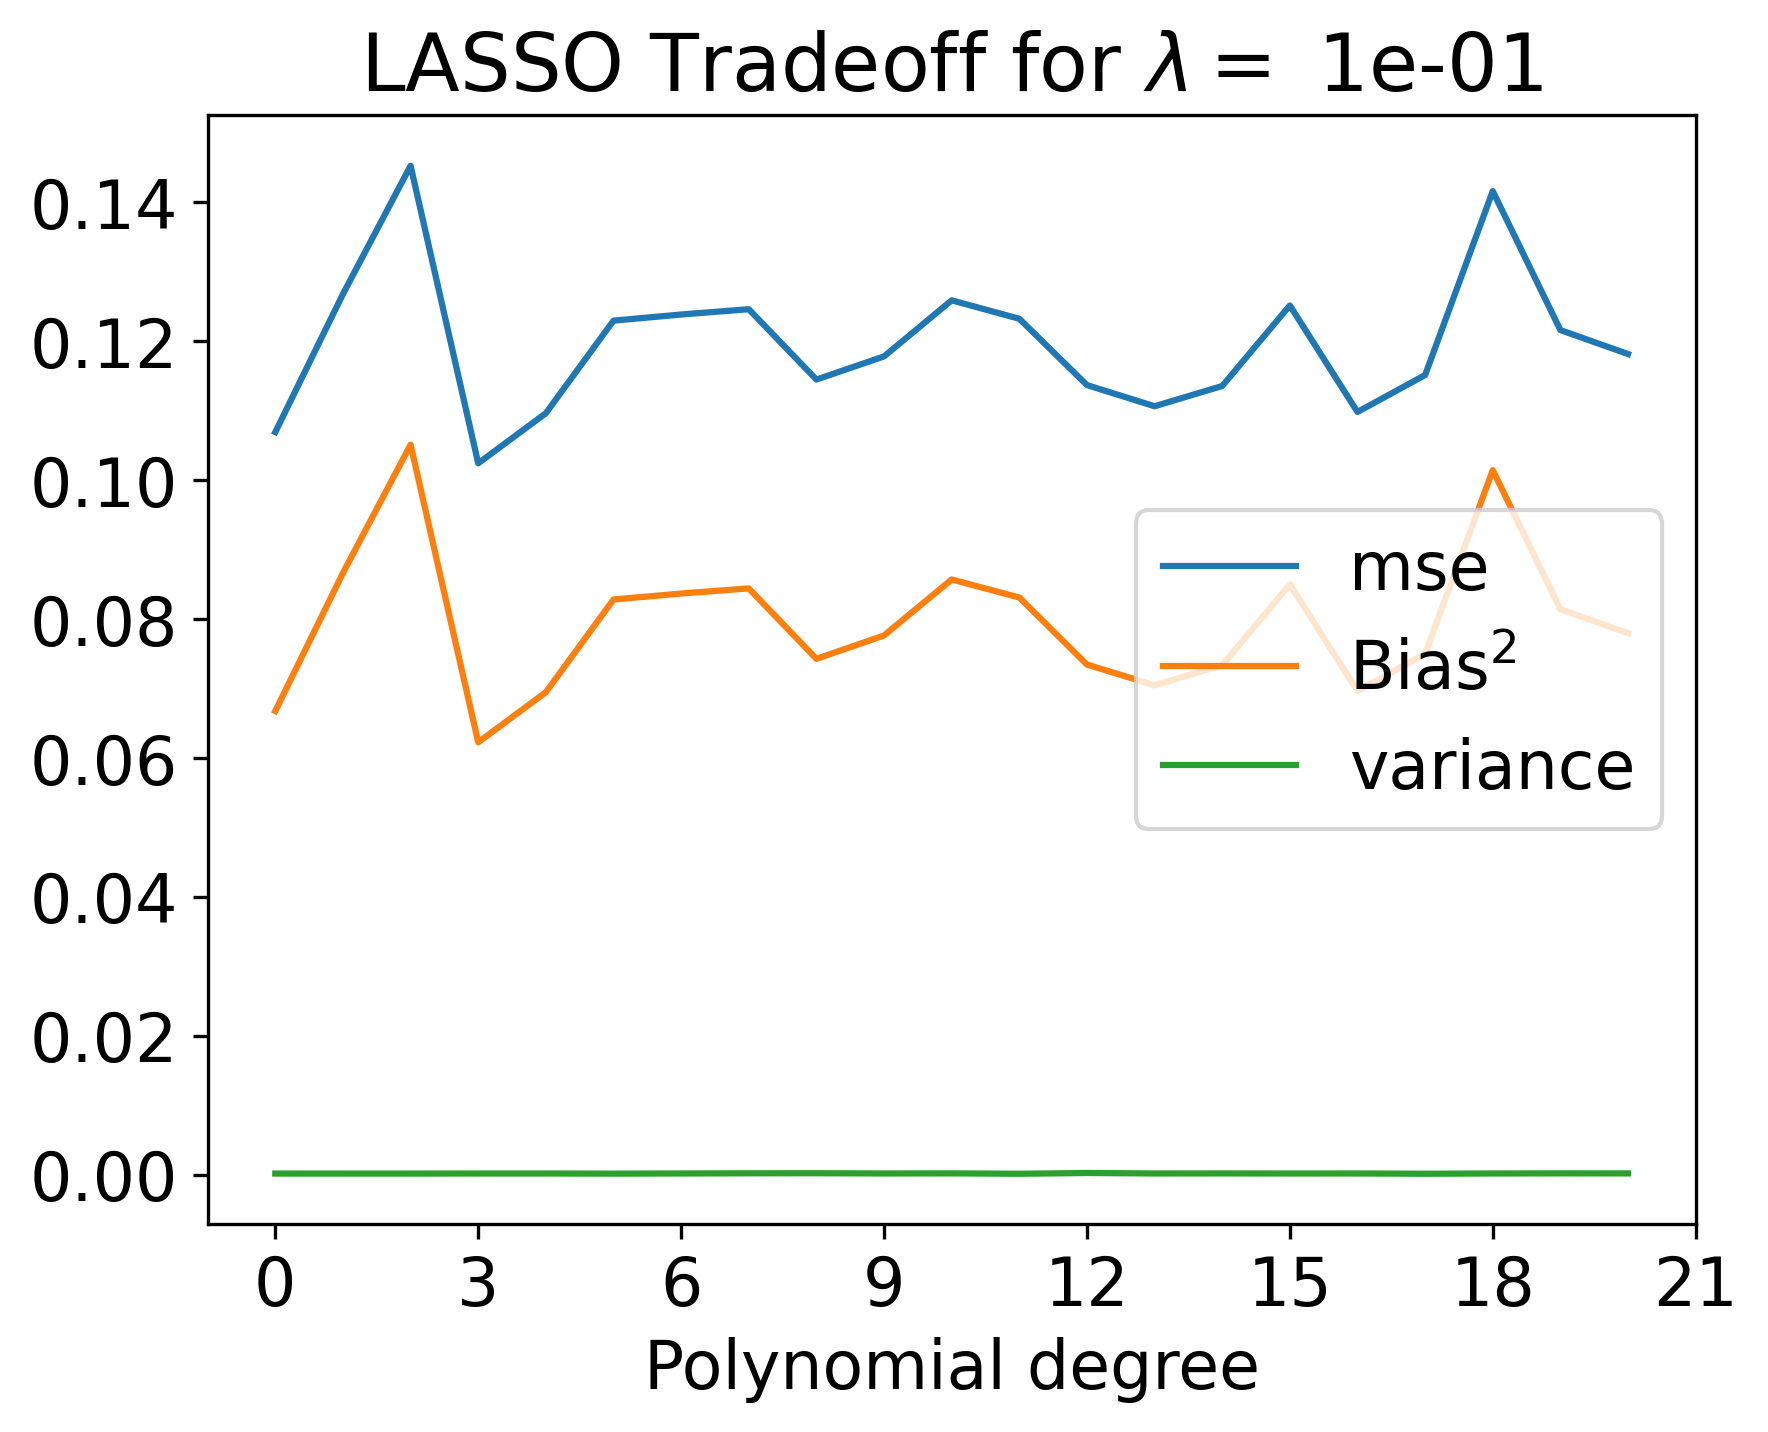
\includegraphics[width=\textwidth]{../figures/tradeoff_LASSO_1e-01_20.png}
    \caption{}
    \label{fig:l_1e-08}
  \end{subfigure}
  \begin{subfigure}{.5\textwidth}
    \centering
    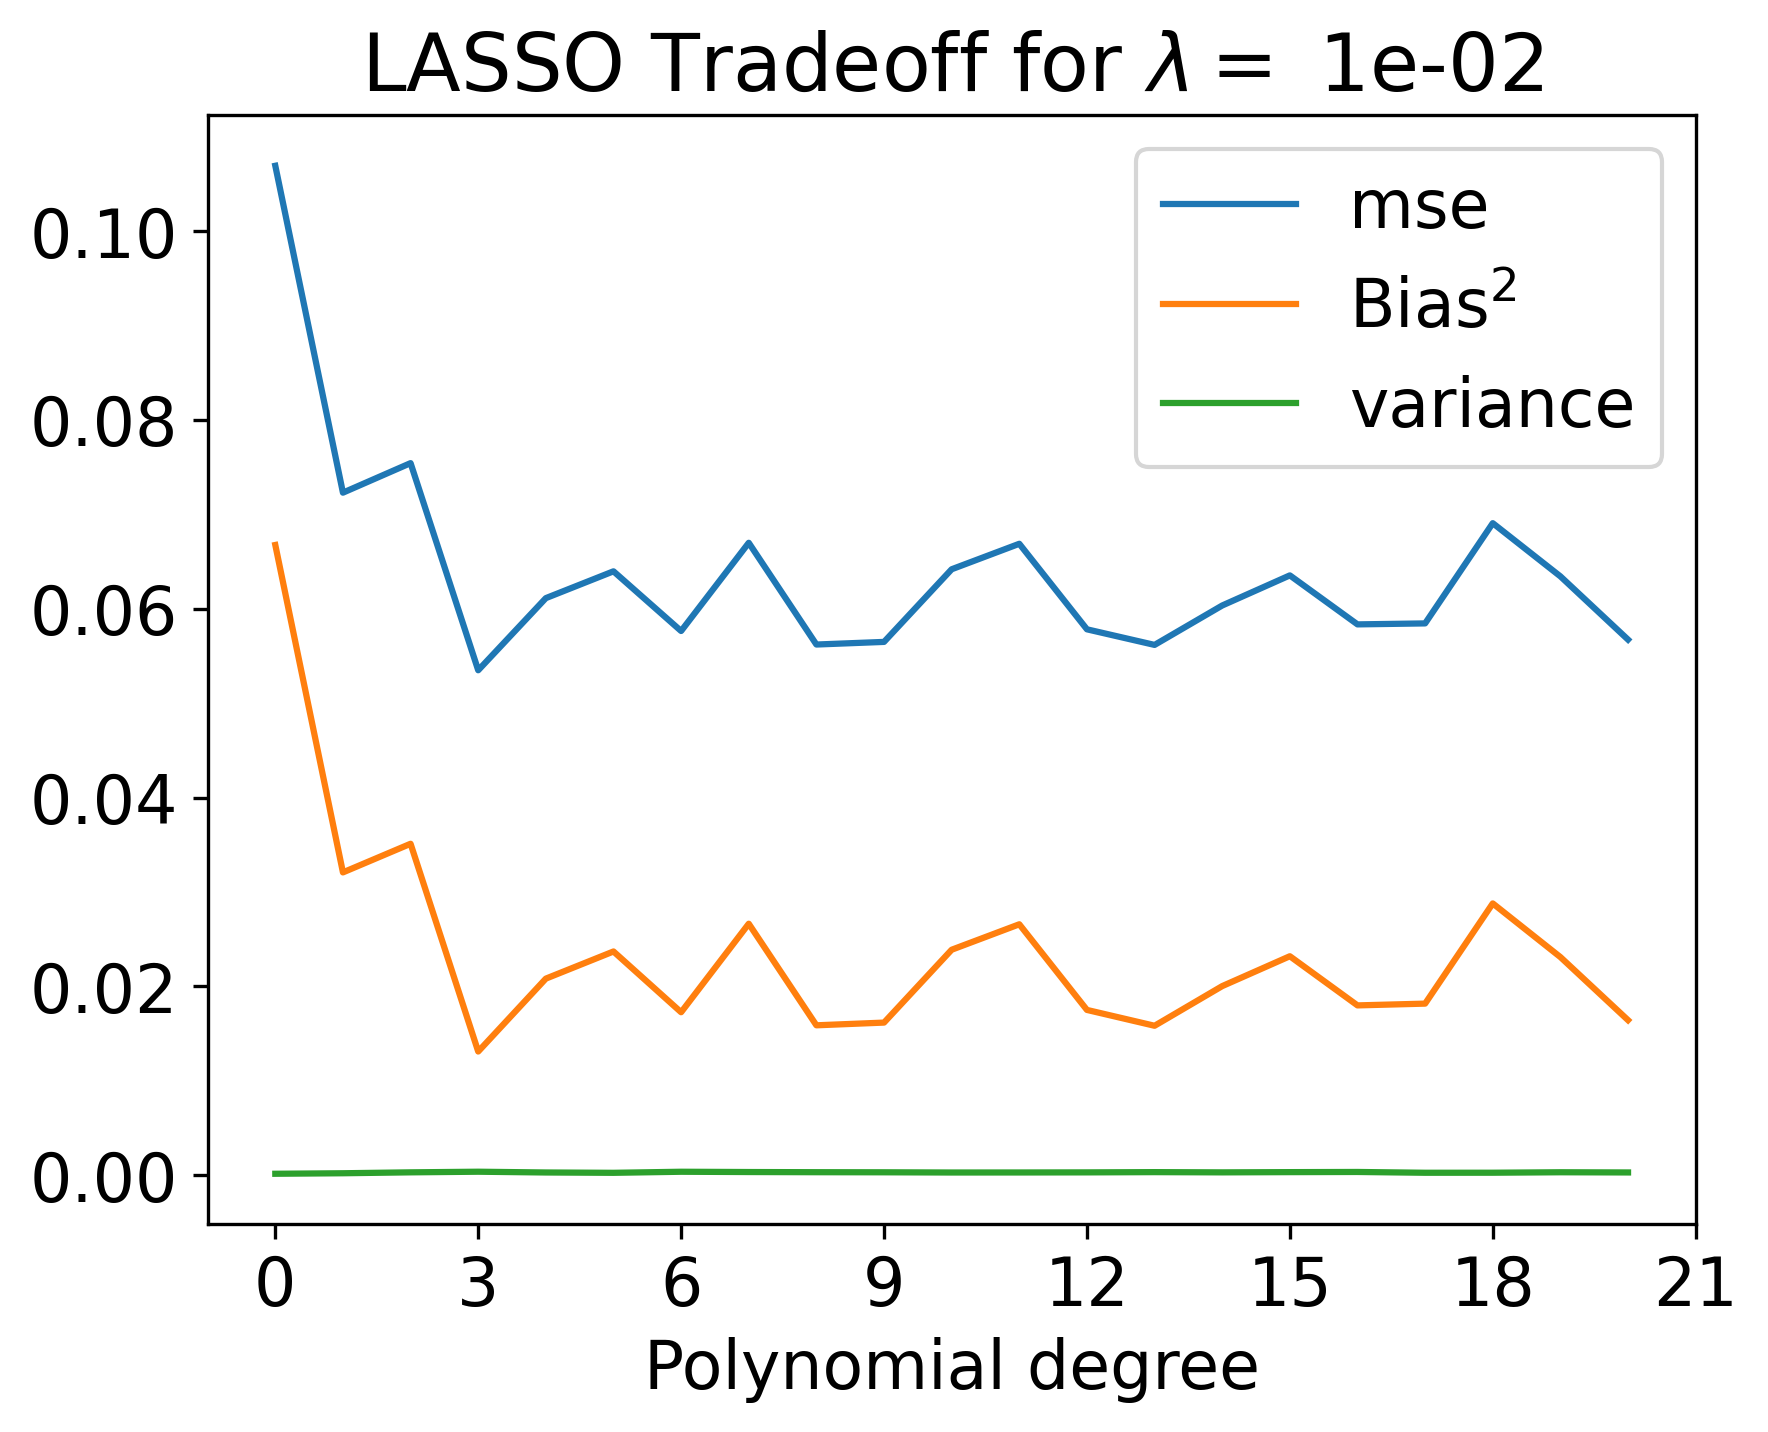
\includegraphics[width=\textwidth]{../figures/tradeoff_LASSO_1e-02_20.png}
    \caption{}
    \label{fig:l_1e-09}
  \end{subfigure}
  \begin{subfigure}{.5\textwidth}
    \centering
    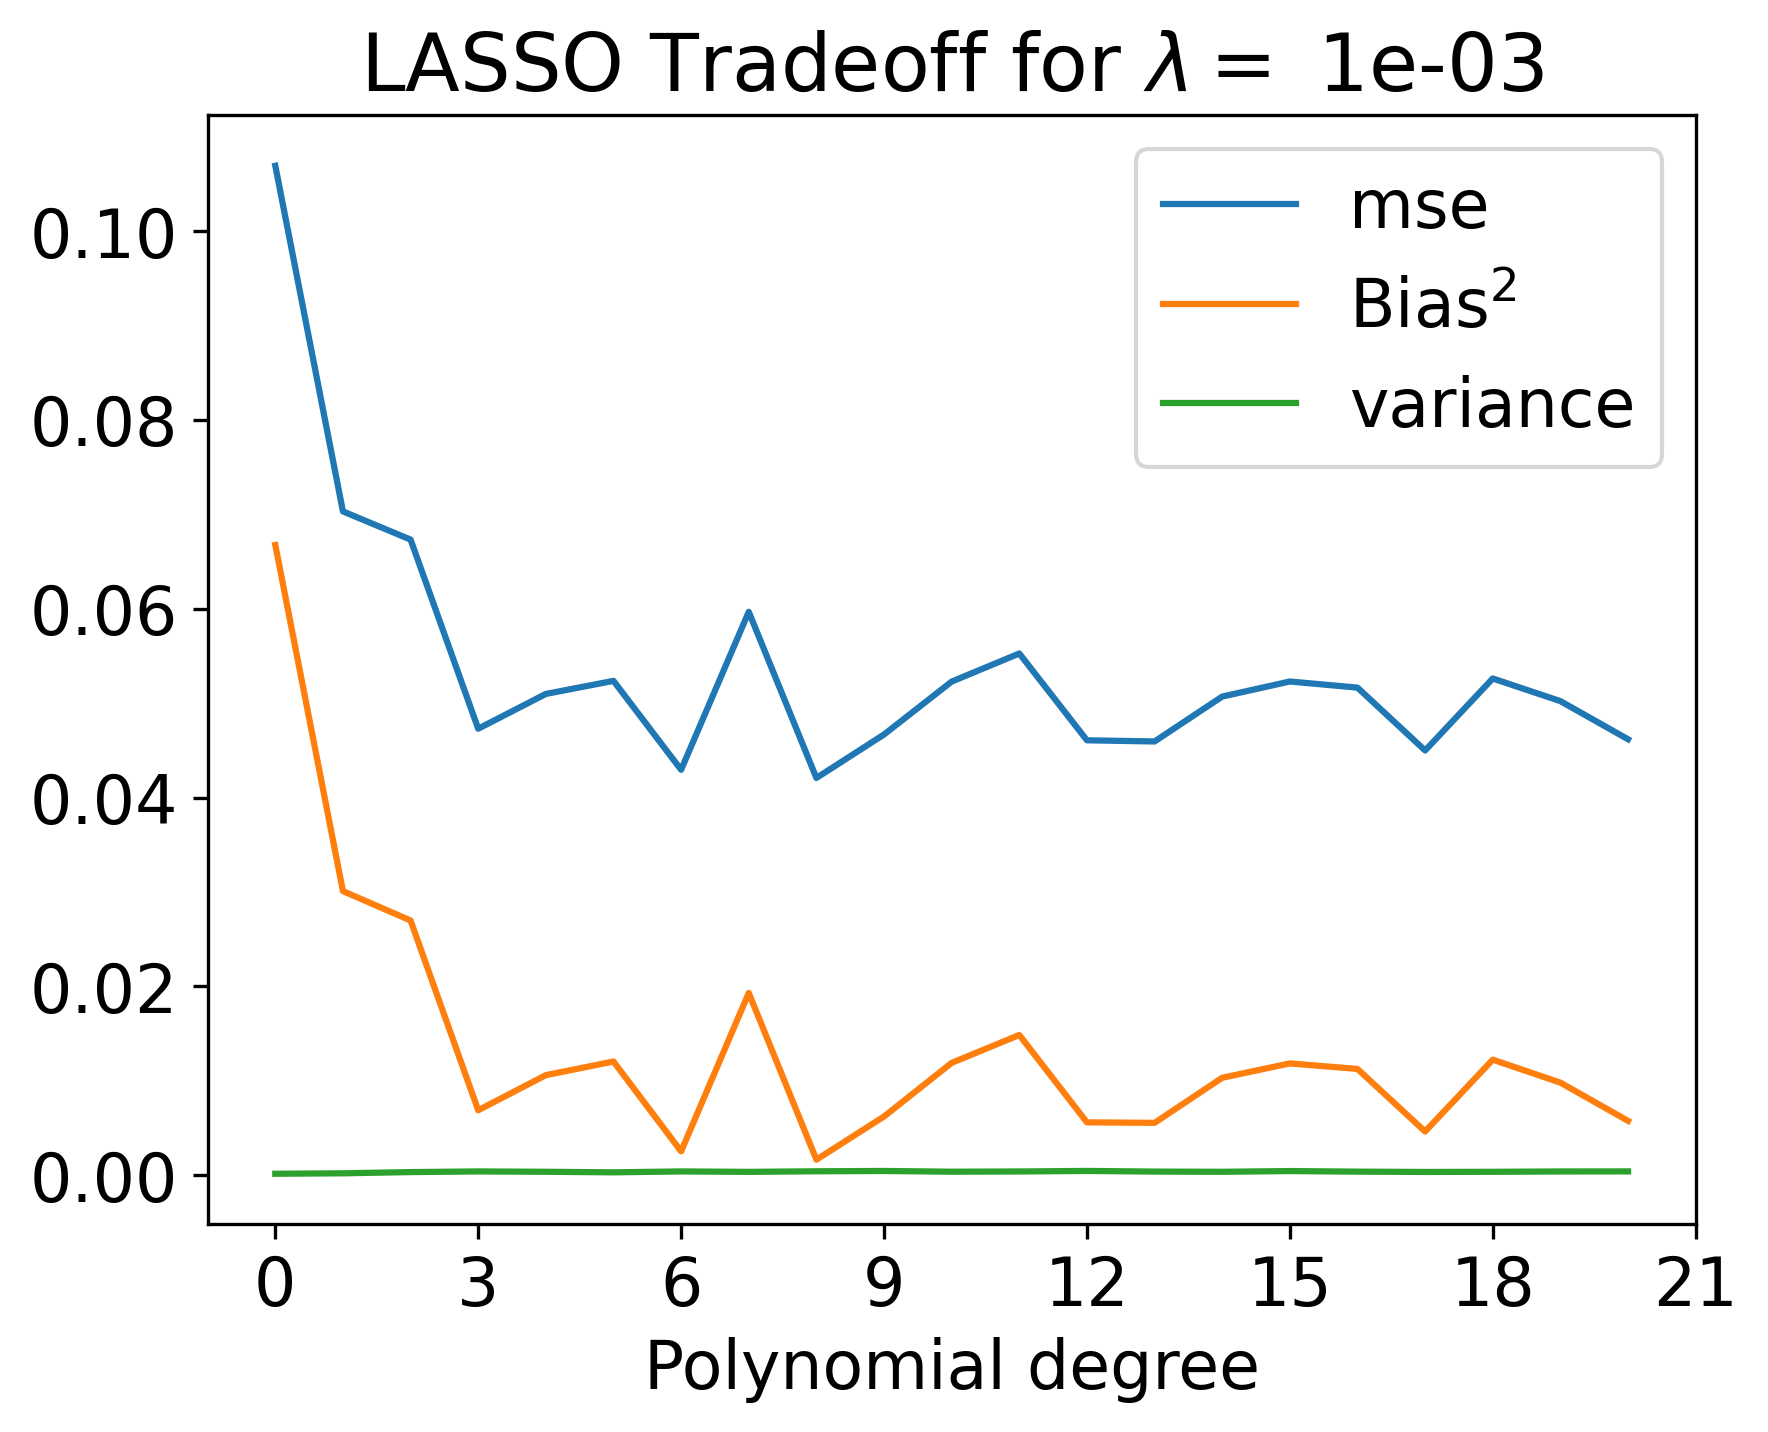
\includegraphics[width=\textwidth]{../figures/tradeoff_LASSO_1e-03_20.png}
    \caption{}
    \label{fig:l_1e-10}
  \end{subfigure}
  \begin{subfigure}{.5\textwidth}
    \centering
    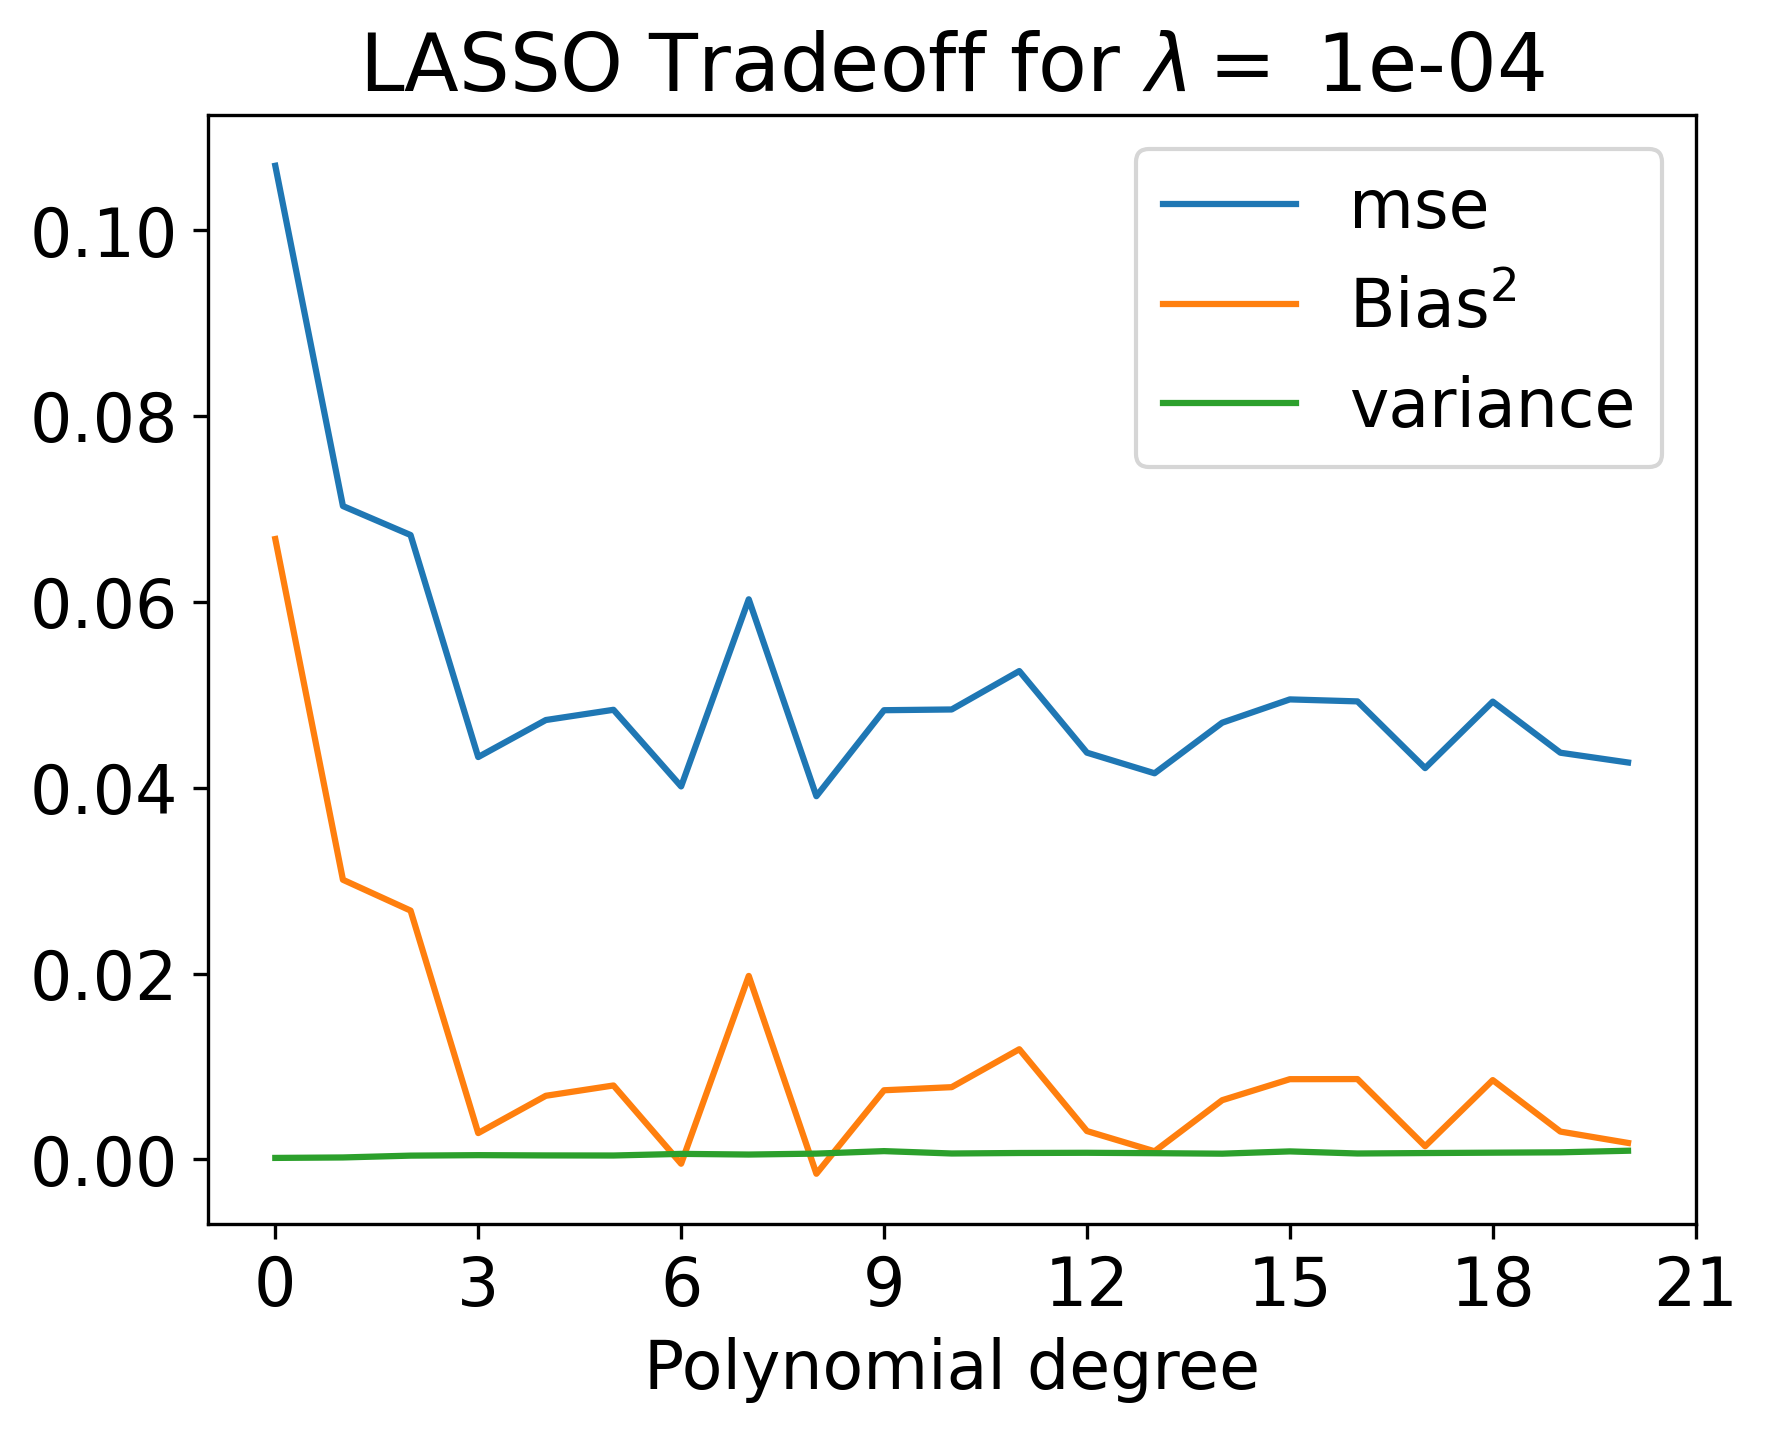
\includegraphics[width=\textwidth]{../figures/tradeoff_LASSO_1e-0420.png}
    \caption{}
    \label{fig:l_1e-1}
  \end{subfigure}
  \begin{subfigure}{.5\textwidth}
    \centering
    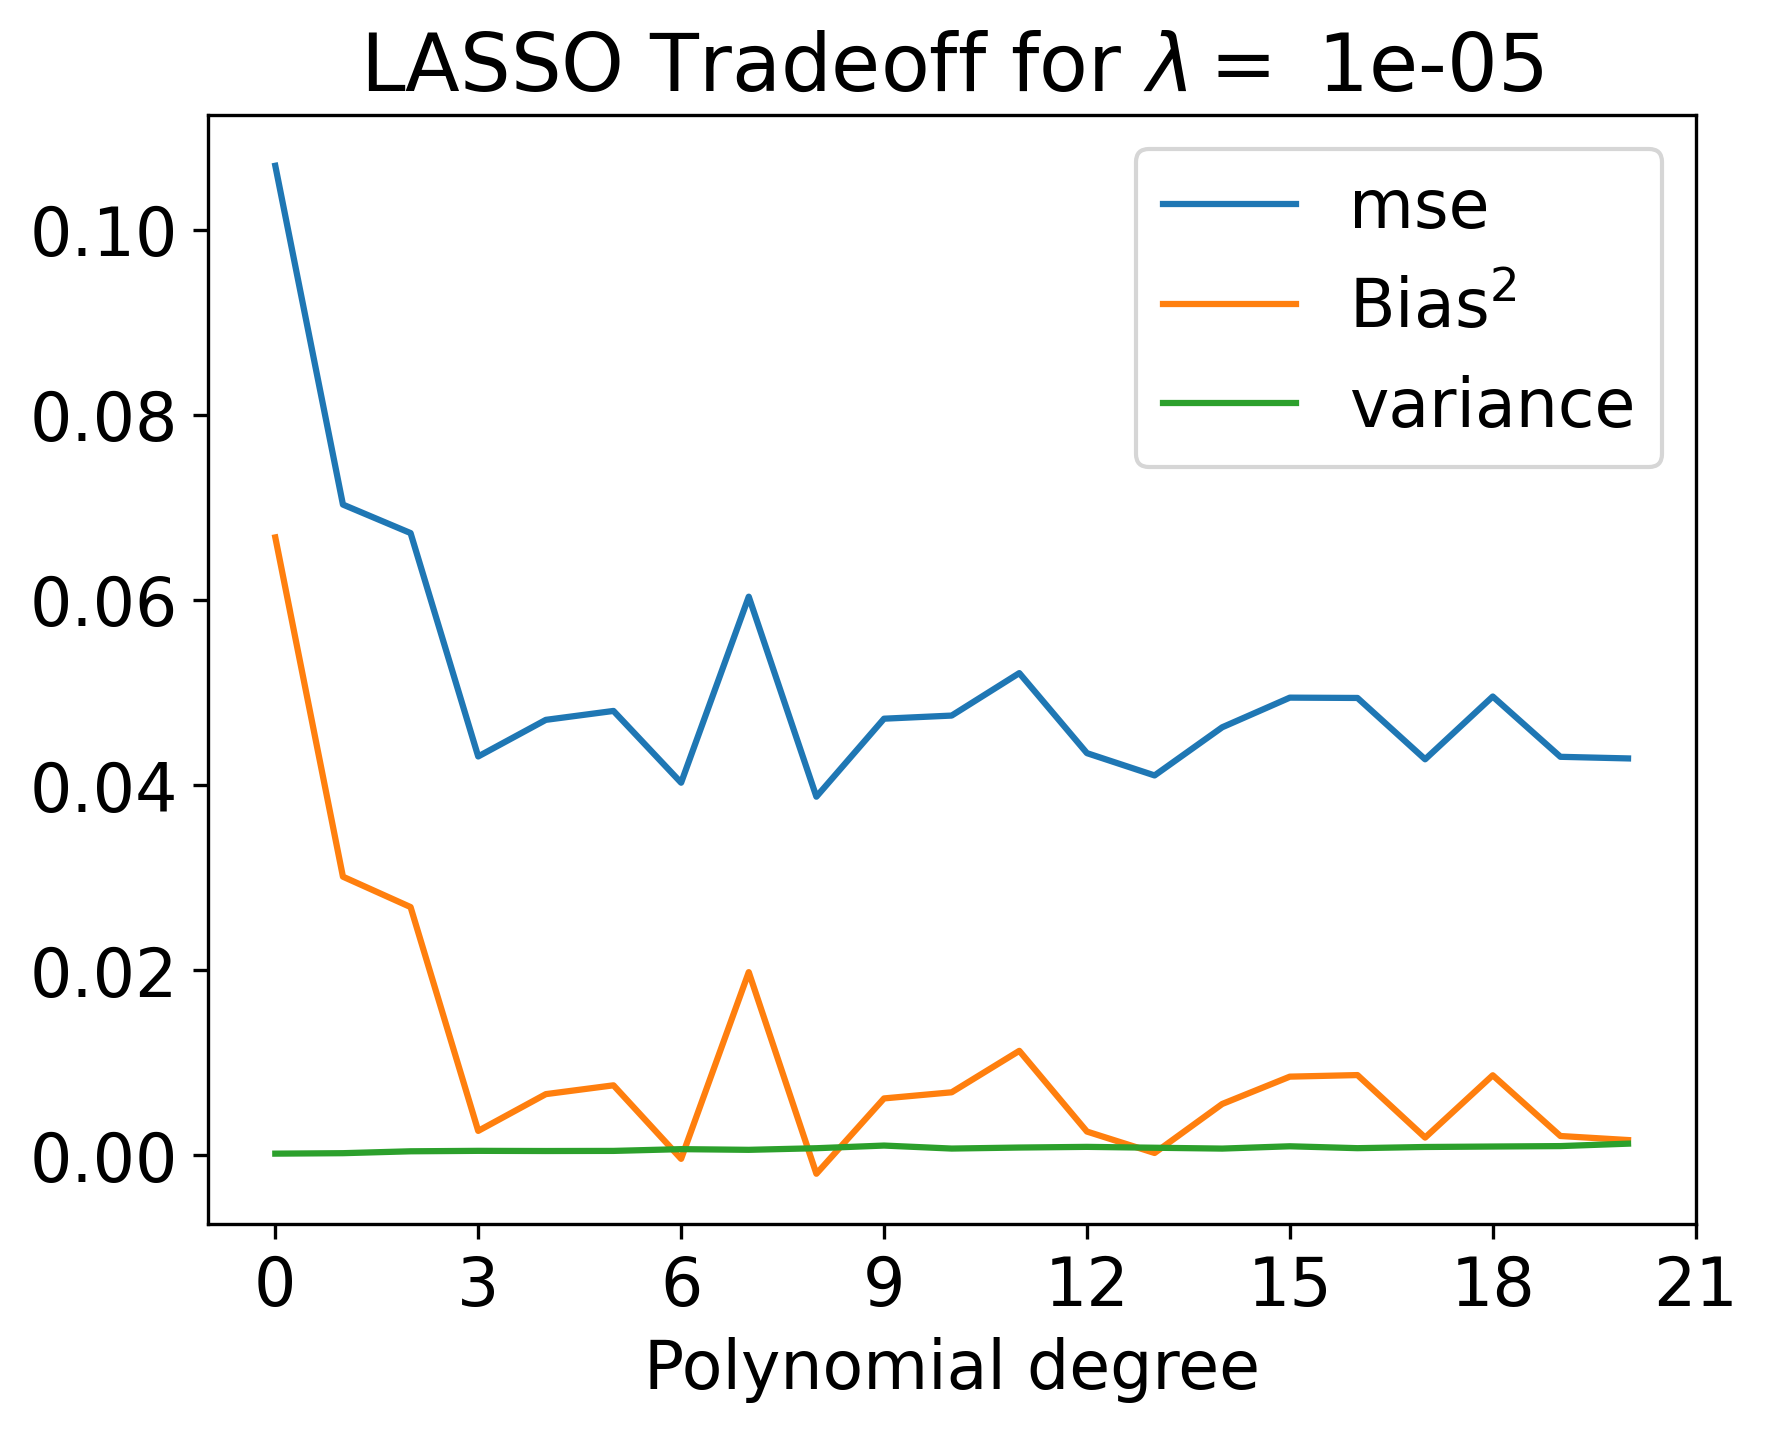
\includegraphics[width=\textwidth]{../figures/tradeoff_LASSO_1e-0520.png}
    \caption{}
    \label{fig:l_1e-12}
  \end{subfigure}
  \begin{subfigure}{.5\textwidth}
    \centering
    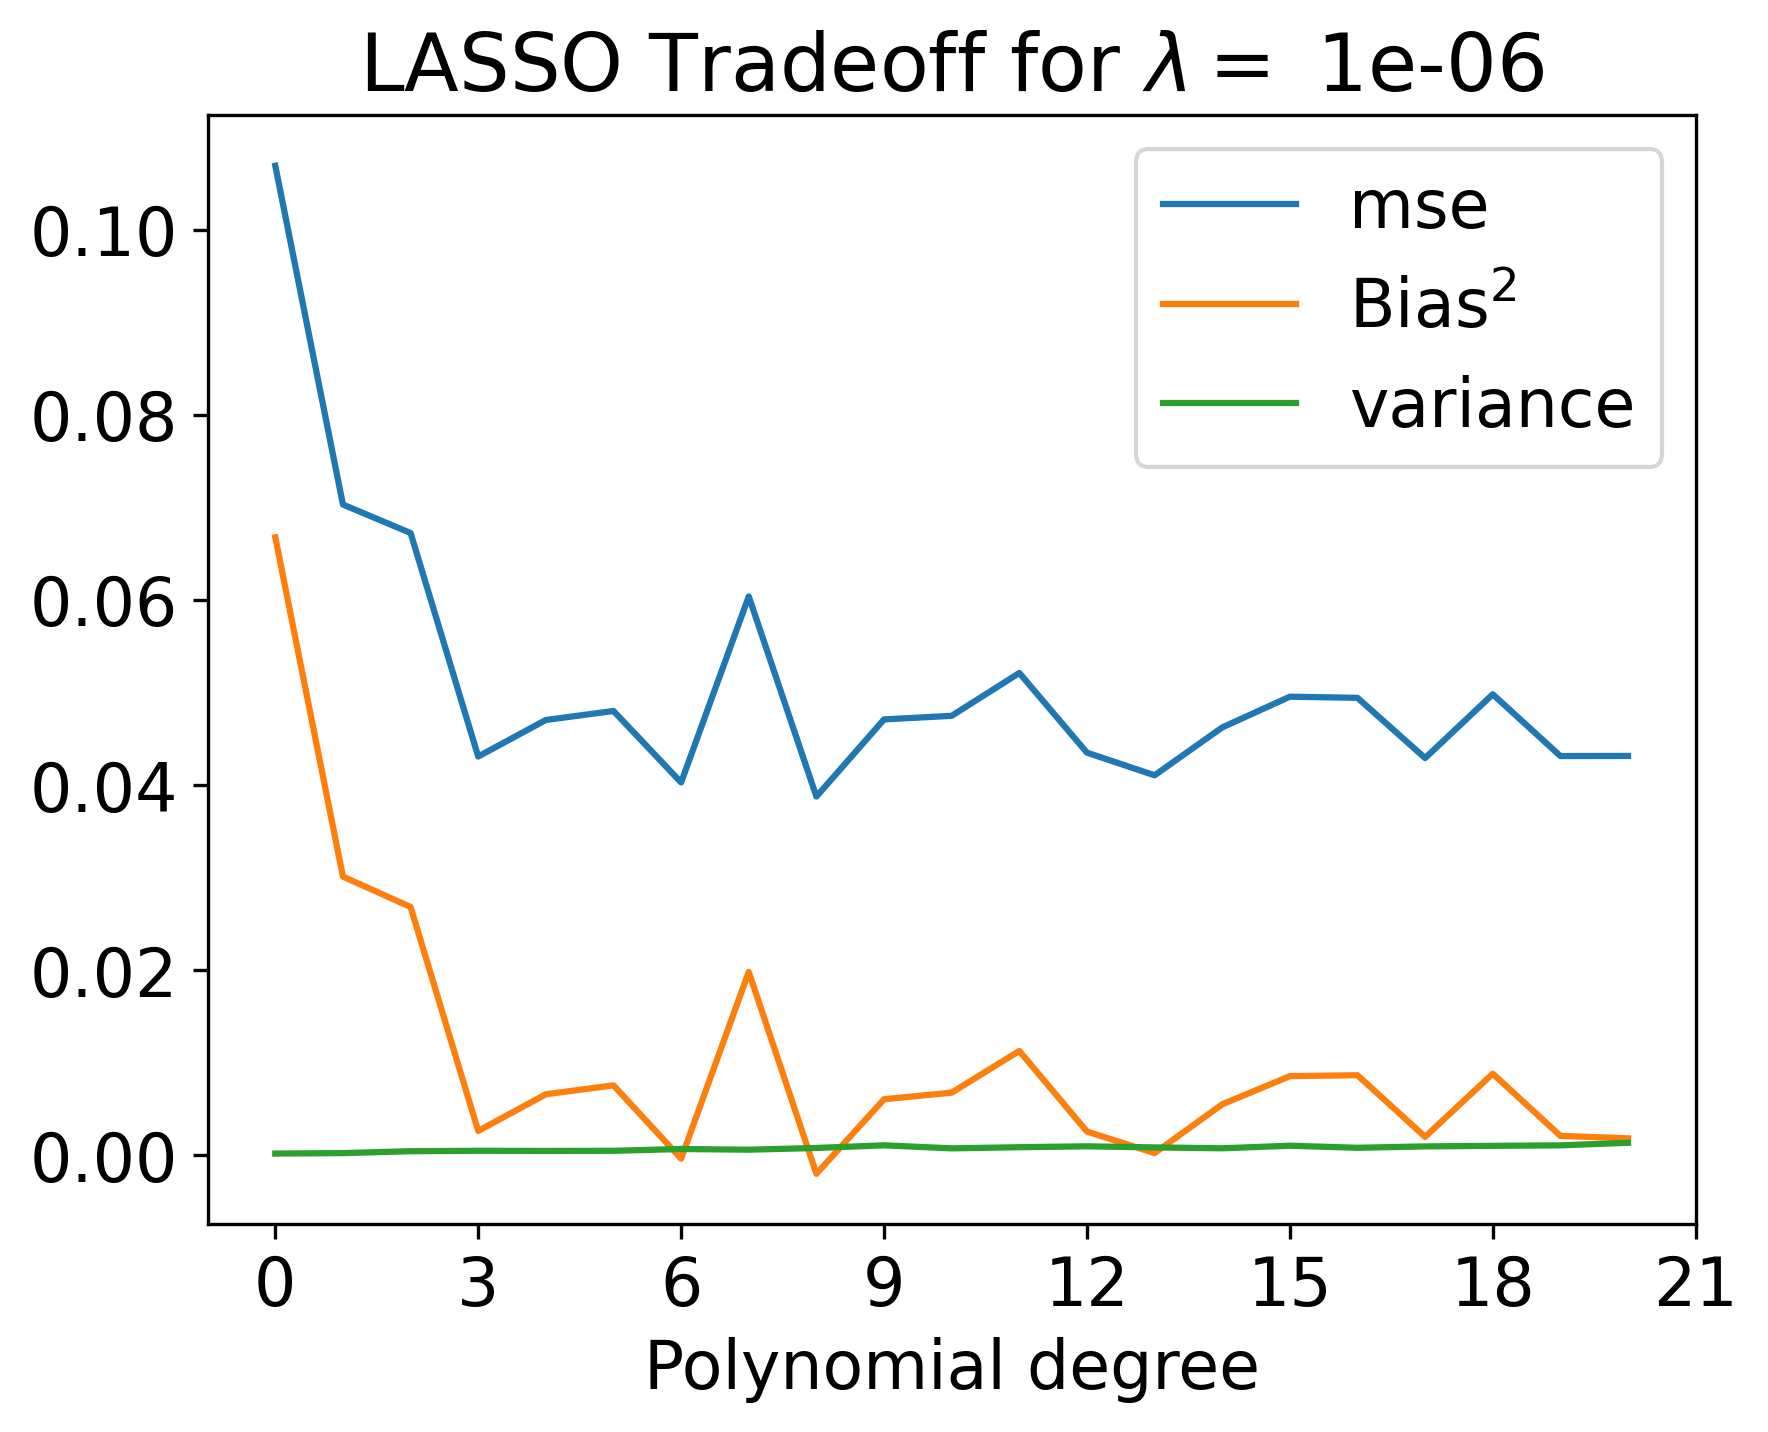
\includegraphics[width=\textwidth]{../figures/tradeoff_LASSO_1e-0620.png}
    \caption{}
    \label{fig:l_1e-13}
  \end{subfigure}
  \caption{Bias-variance tradeoff for different choices of lambda using Lasso regression for data with $n=30$ steps and noise standard deviation of $\sigma=0.2$}
  \label{fig:lasso_tradeoff}
\end{figure}
When comparing the two above figures (\ref{fig:ridge_tradeoff} and \ref{fig:lasso_tradeoff}) of the bias variance tradeoff with the tradeoff for OLS in figure \ref{fig:bias_variance} we see that ridge and lasso are much less prone to a fast increasing variance for higher degrees when using smaller $\lambda$. It is also clear that the lasso regression is even better at keeping the variance down than the ridge regression especially for larger $\lambda$ parameters. We can also see that there is minimal change in lasso for a change in $\lambda$ where the bias remains the greater contributing factor to the error even for higher degrees. It is in other words clear that the dampening parameter $\lambda$ does a great job of reducing overfitting especially for Lasso but also for Ridge regression with larger $\lambda$ parameters.

\subsubsection{Cross validation}
From the implementation of cross validation we get the following comparison plot in figure \ref{fig:cv_comp} for data with $n=30$ steps and $\sigma=0.2$ for 100 bootstrap iterations compared to cross validation of both 5 and 10 $k$-folds:
\begin{figure}[H]
  \begin{subfigure}{.5\textwidth}
    \centering
    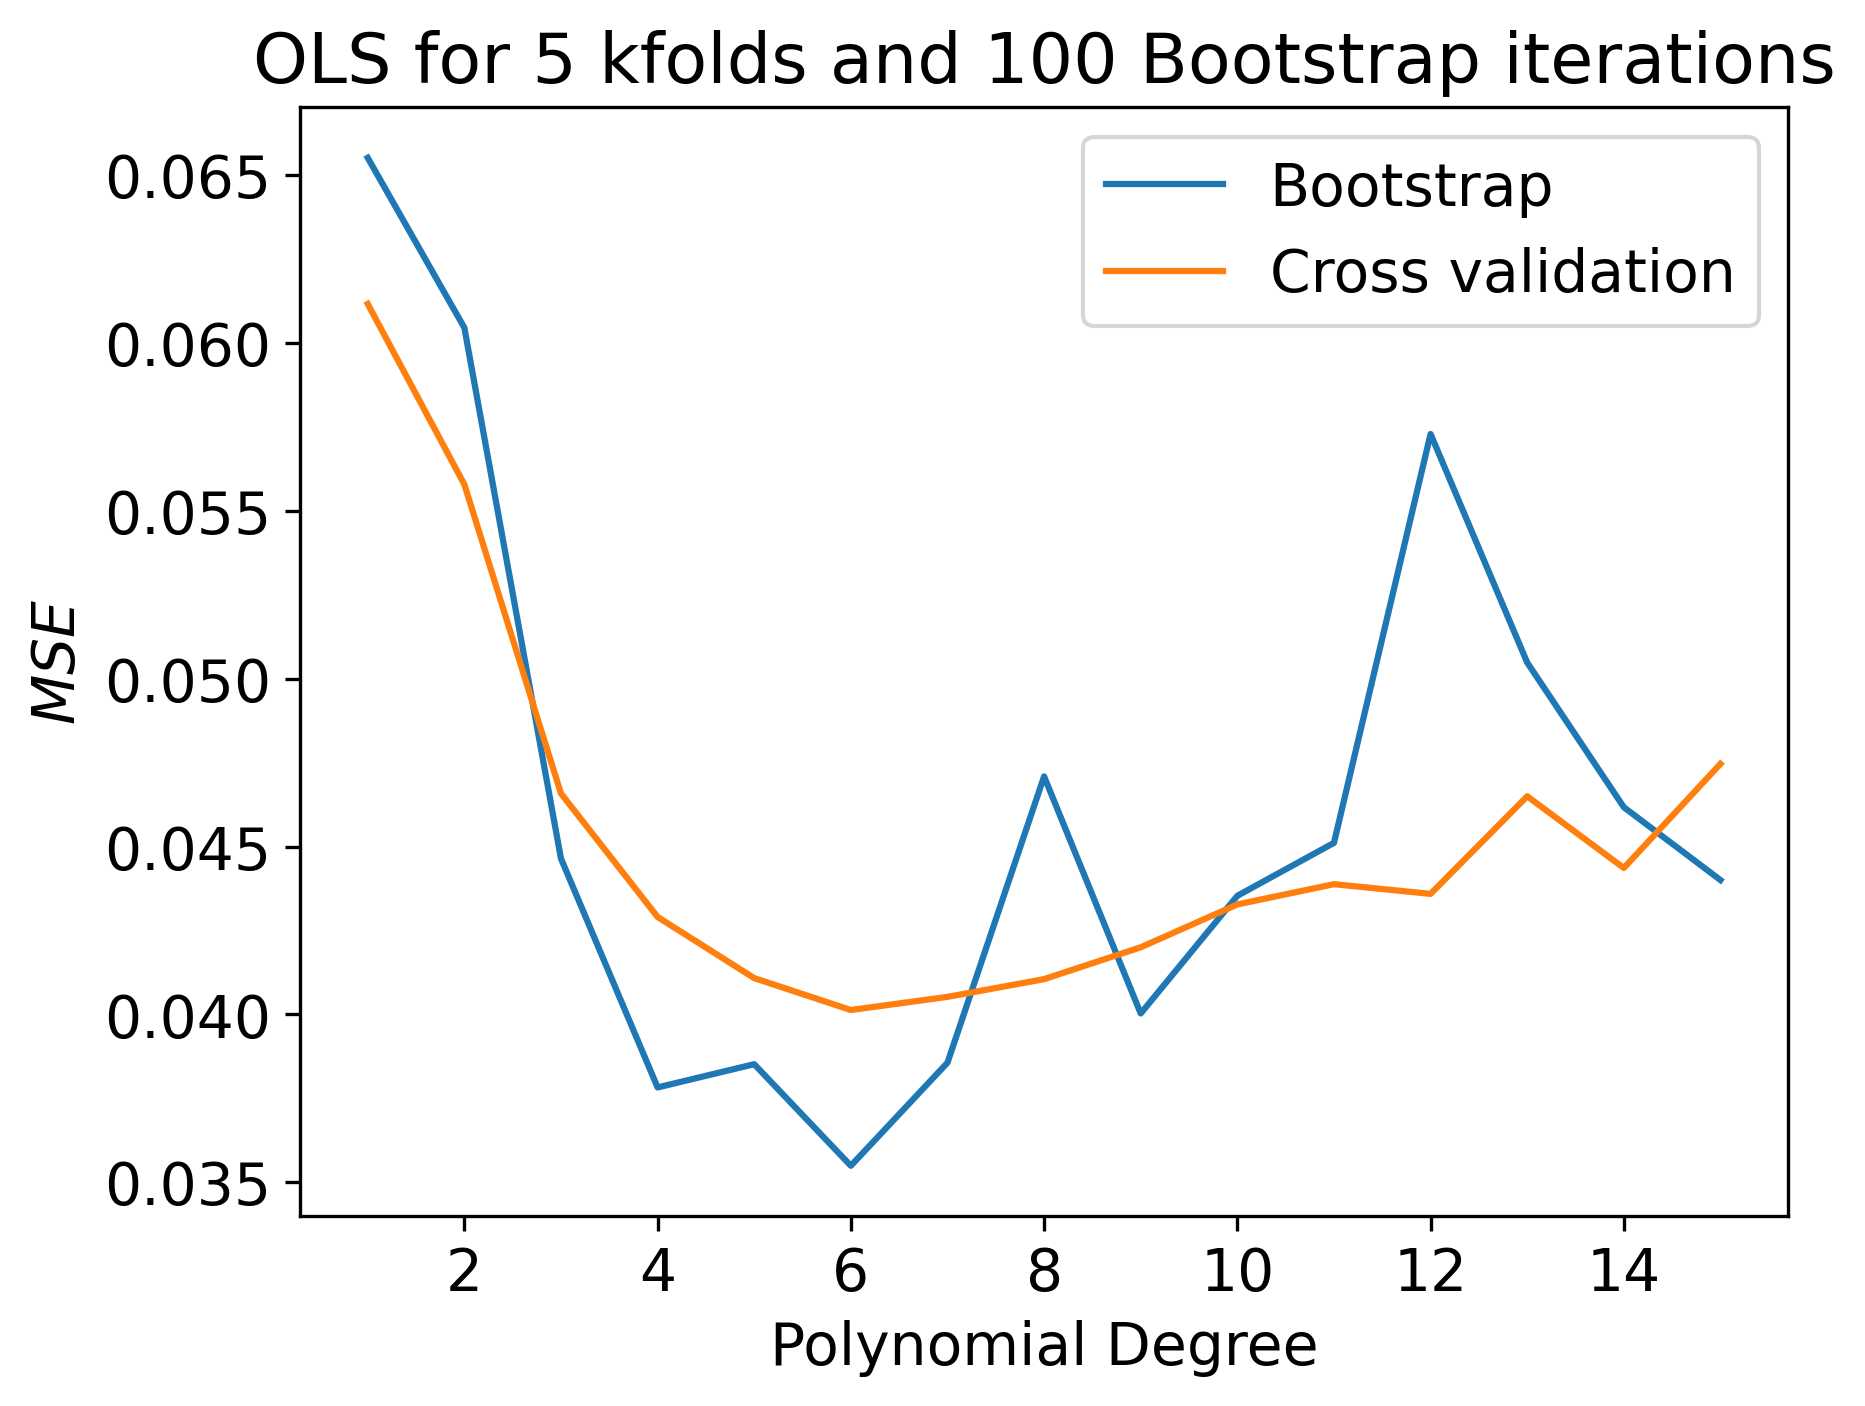
\includegraphics[width=\textwidth]{../figures/boot_cv_comp_OLS_100_5.png}
    \caption{5 $k$-folds}
    \label{fig:cv_b_comp_5}
  \end{subfigure}
  \begin{subfigure}{.5\textwidth}
    \centering
    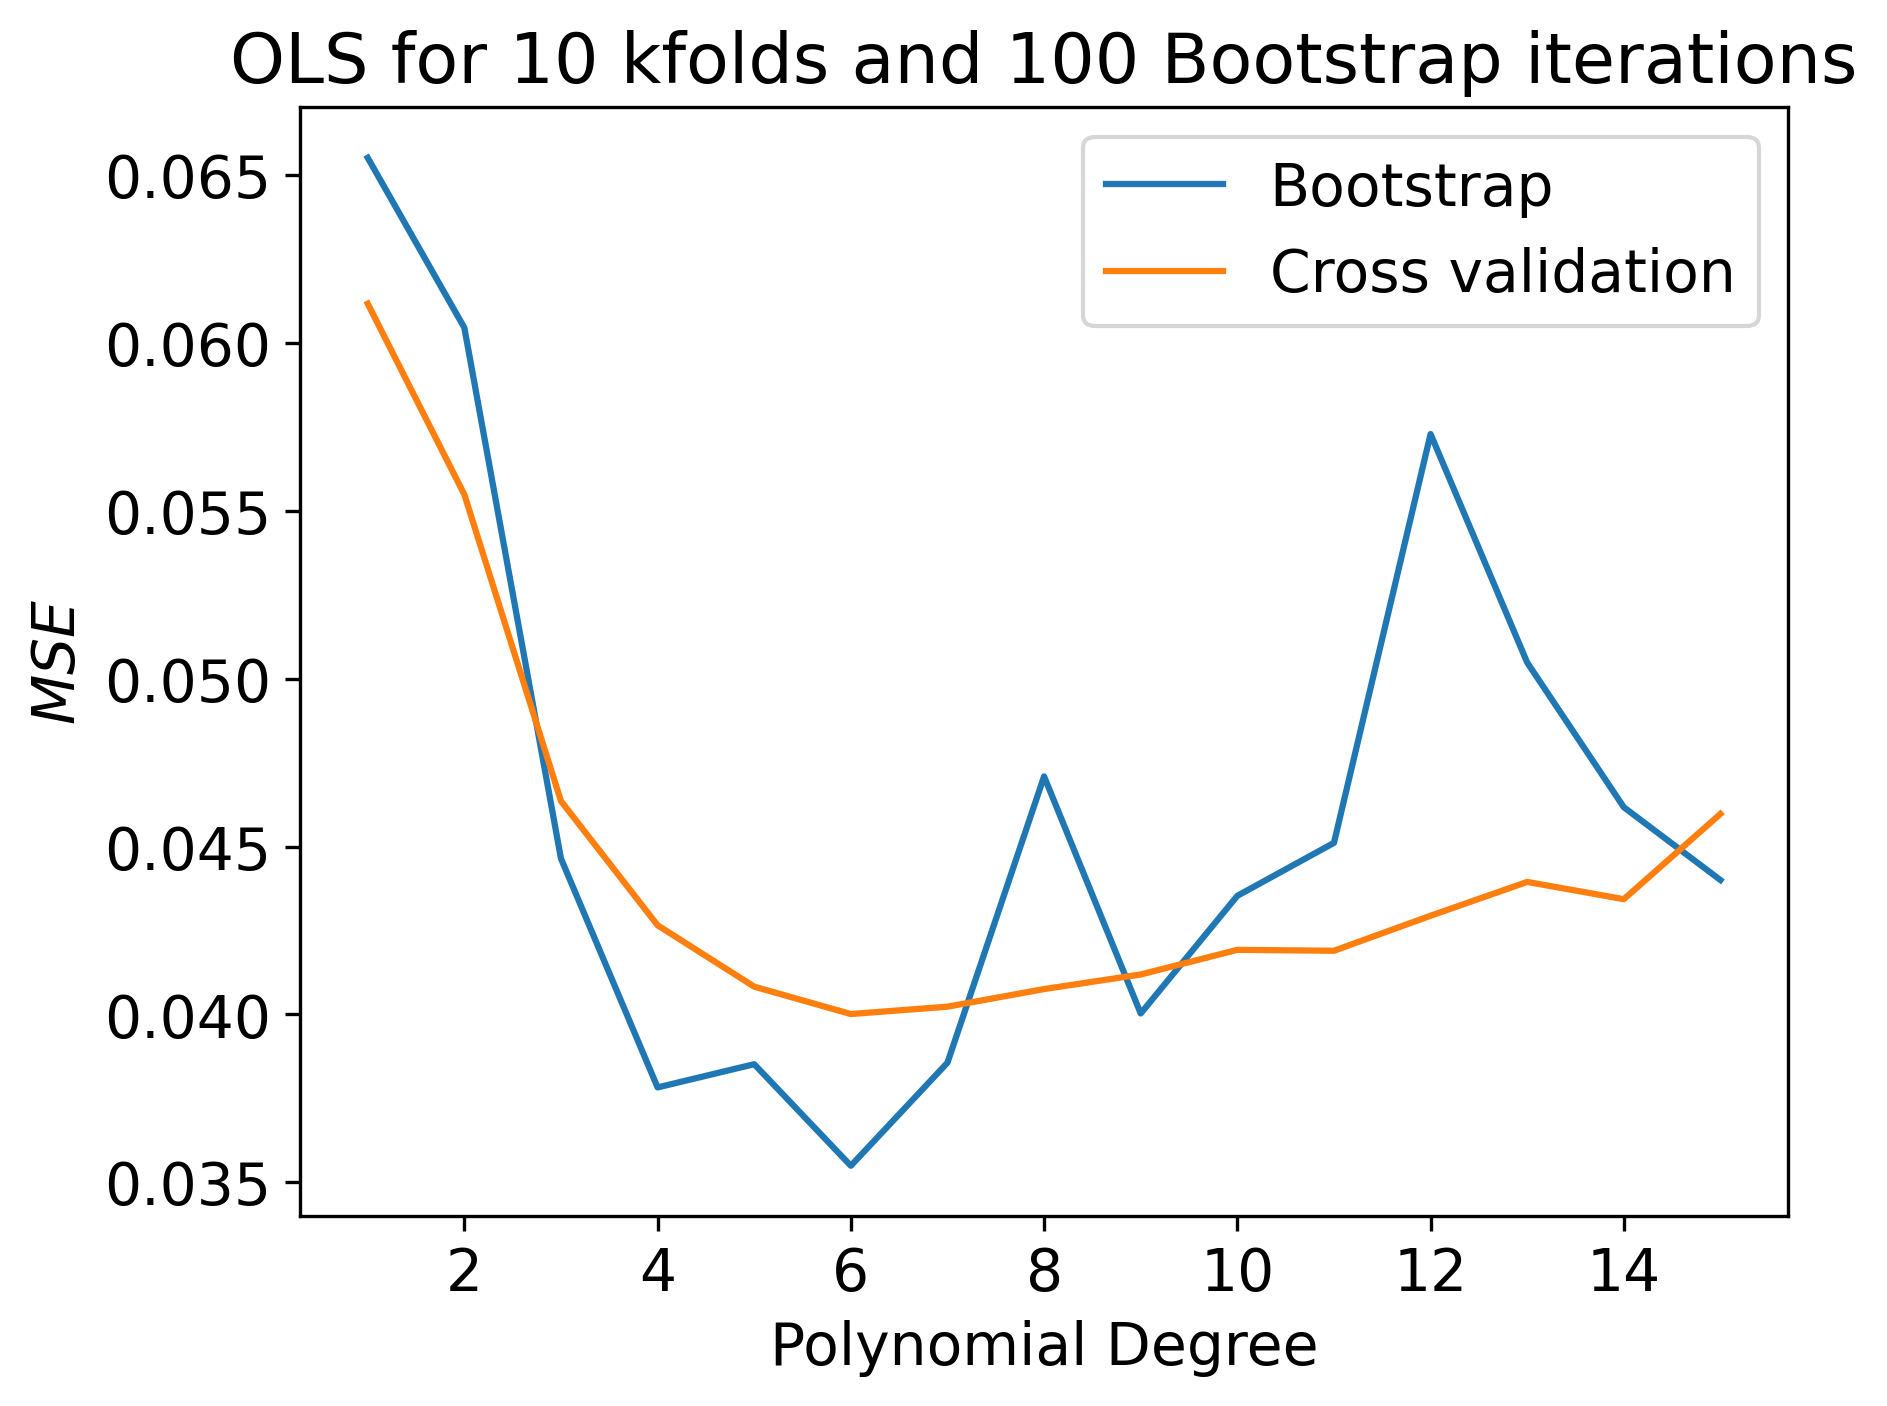
\includegraphics[width=\textwidth]{../figures/boot_cv_comp_OLS_100_10.png}
    \caption{10 $k$-folds}
    \label{fig:cv_b_comp_10}
  \end{subfigure}
  \caption{A comparison between bootstrap and cross validation for datasets with $n=30$ steps, noise standard deviation $\sigma=0.2$ and 100 bootstrap iterations}
  \label{fig:cv_comp}
\end{figure}
We see different results for bootstrap and cross validation for both 5 and 10 $k$-folds. The difference between the $k$-folds are quite small, but the difference from the bootstrap is for some polynomial degrees higher than others. This is especially true for lower polynomial degrees where bootstrap gives lower MSE, and for higher polynomial degrees where bootstrap gives higher MSE. Under in figure \ref{fig:cv_comp_01} we see a comparison for the same amount of data only with an error standard deviation of $\sigma=0.1$ instead of 0.2:
\begin{figure}[H]
  \centering
  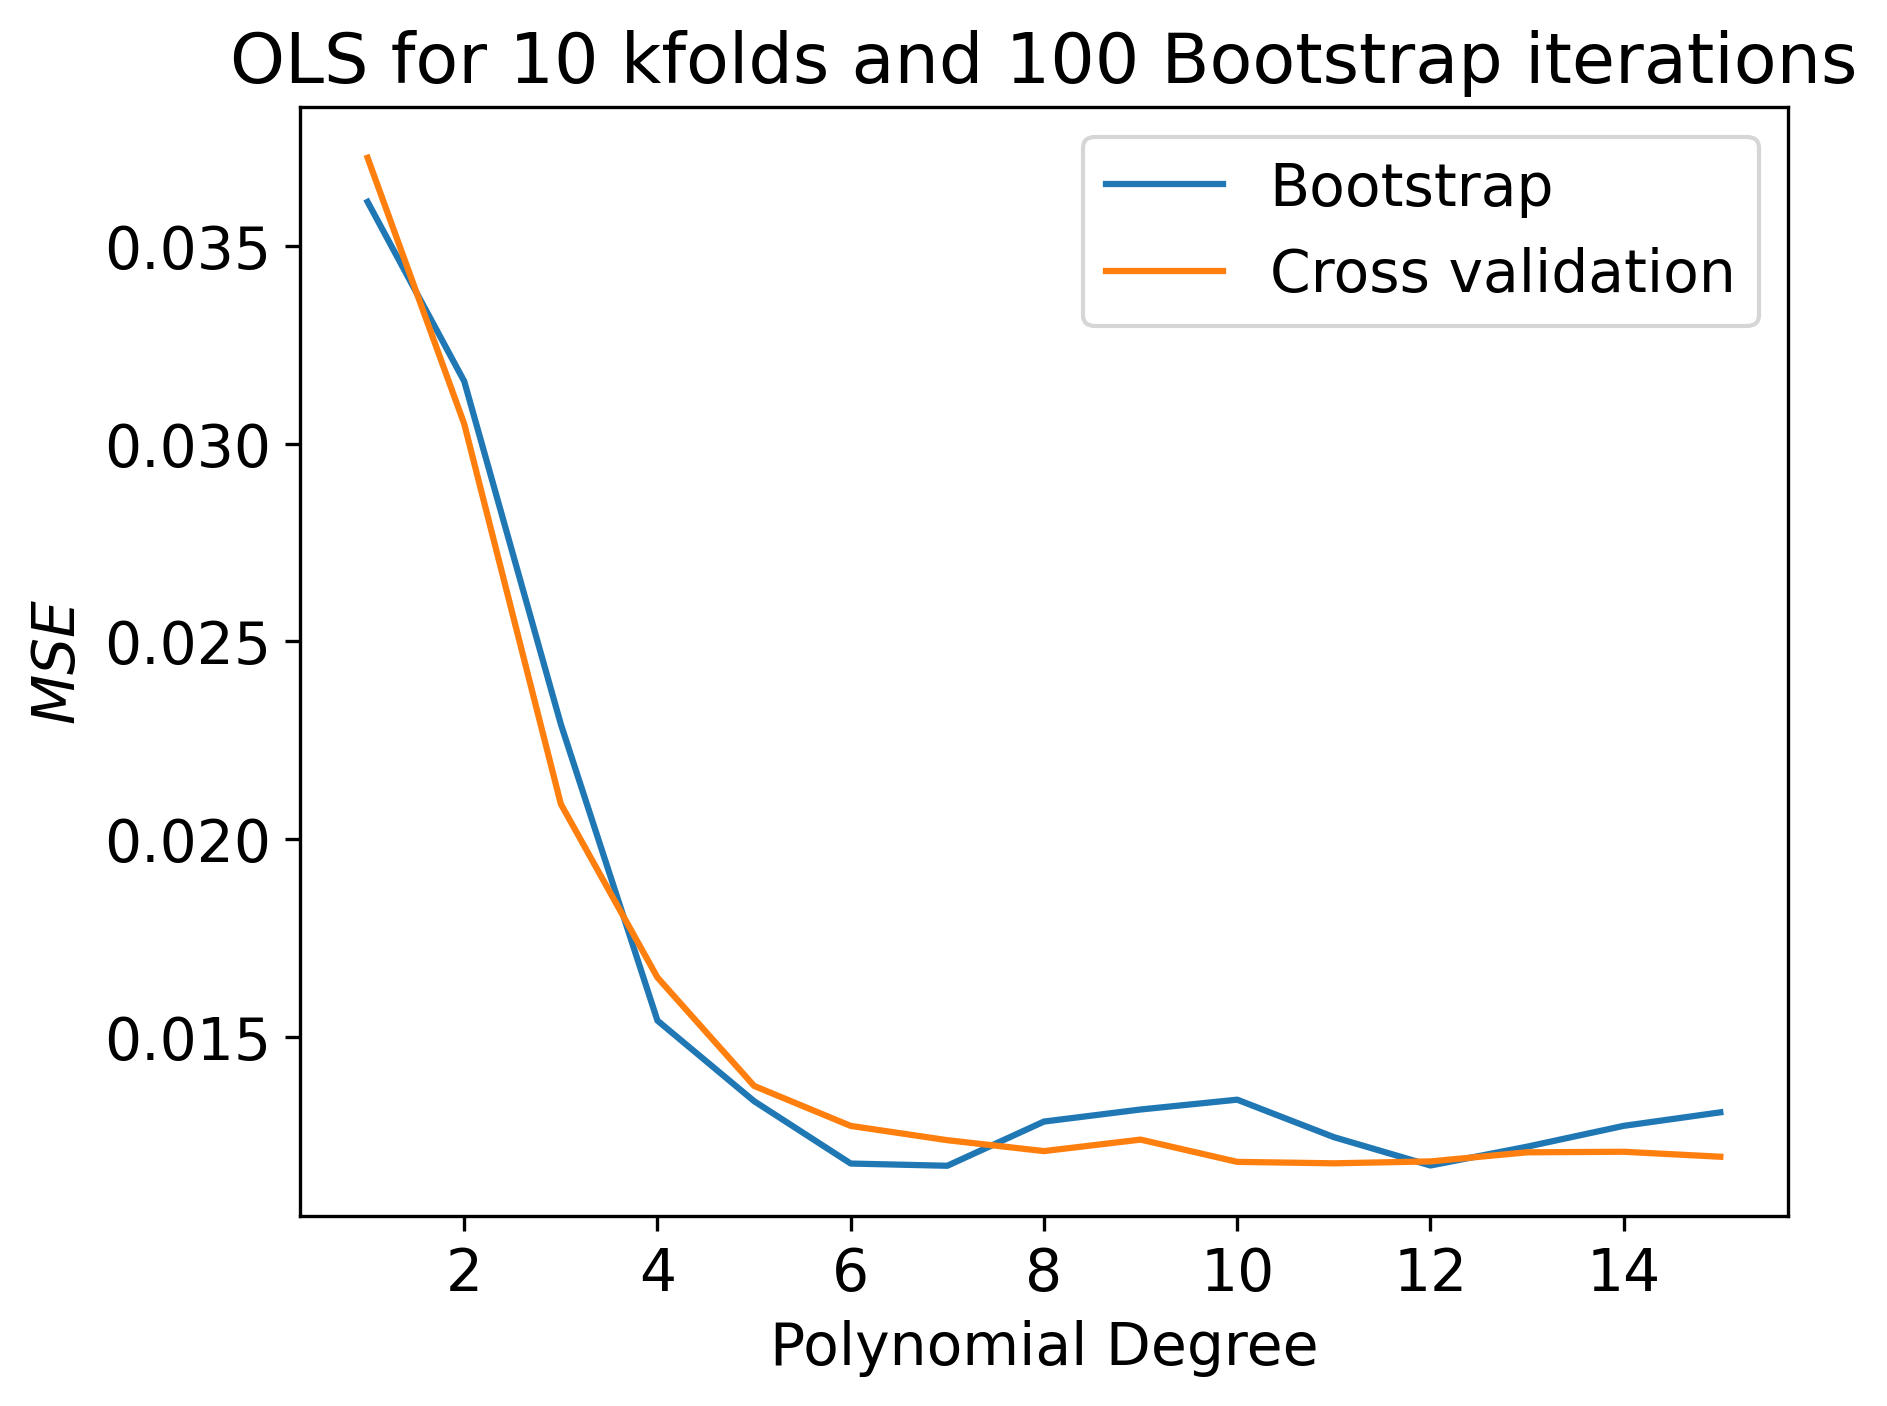
\includegraphics[width=.7\textwidth]{../figures/boot_cv_comp_01.png}
  \caption{A comparison between bootstrap and cross validation for datasets with $n=30$ steps, noise standard deviation $\sigma=0.1$ and 100 bootstrap iterations}
  \label{fig:cv_comp_01}
\end{figure}
We see above in figure \ref{fig:cv_comp_01} that the bootstrap gives more similar results to the cross validation method for a lower noise standard deviation. At the same time we see the same trend for the bootstrap with lower MSE values around a degree of 6 and 12 while it still gives higher MSE for around a degree of 10 and above 13.

\subsubsection{Finding best models}
We continue analyzing our models error dependency on polynomial degree and choice of the parameter $\lambda$. To best show this for lasso and ridge regression a heatmap is shown in figure \ref{fig:heat_franke} below where cross validation with 5 $k$-folds has been used. Here we have polynomial degrees on the x-axis and $\lambda$ on the y-axis together with the MSE in color following the colorbar to the right of the figures. We can also see in figure \ref{fig:best_OLS} the same analysis for OLS without the $\lambda$ dependence.
\begin{figure}[H]
  \centering
  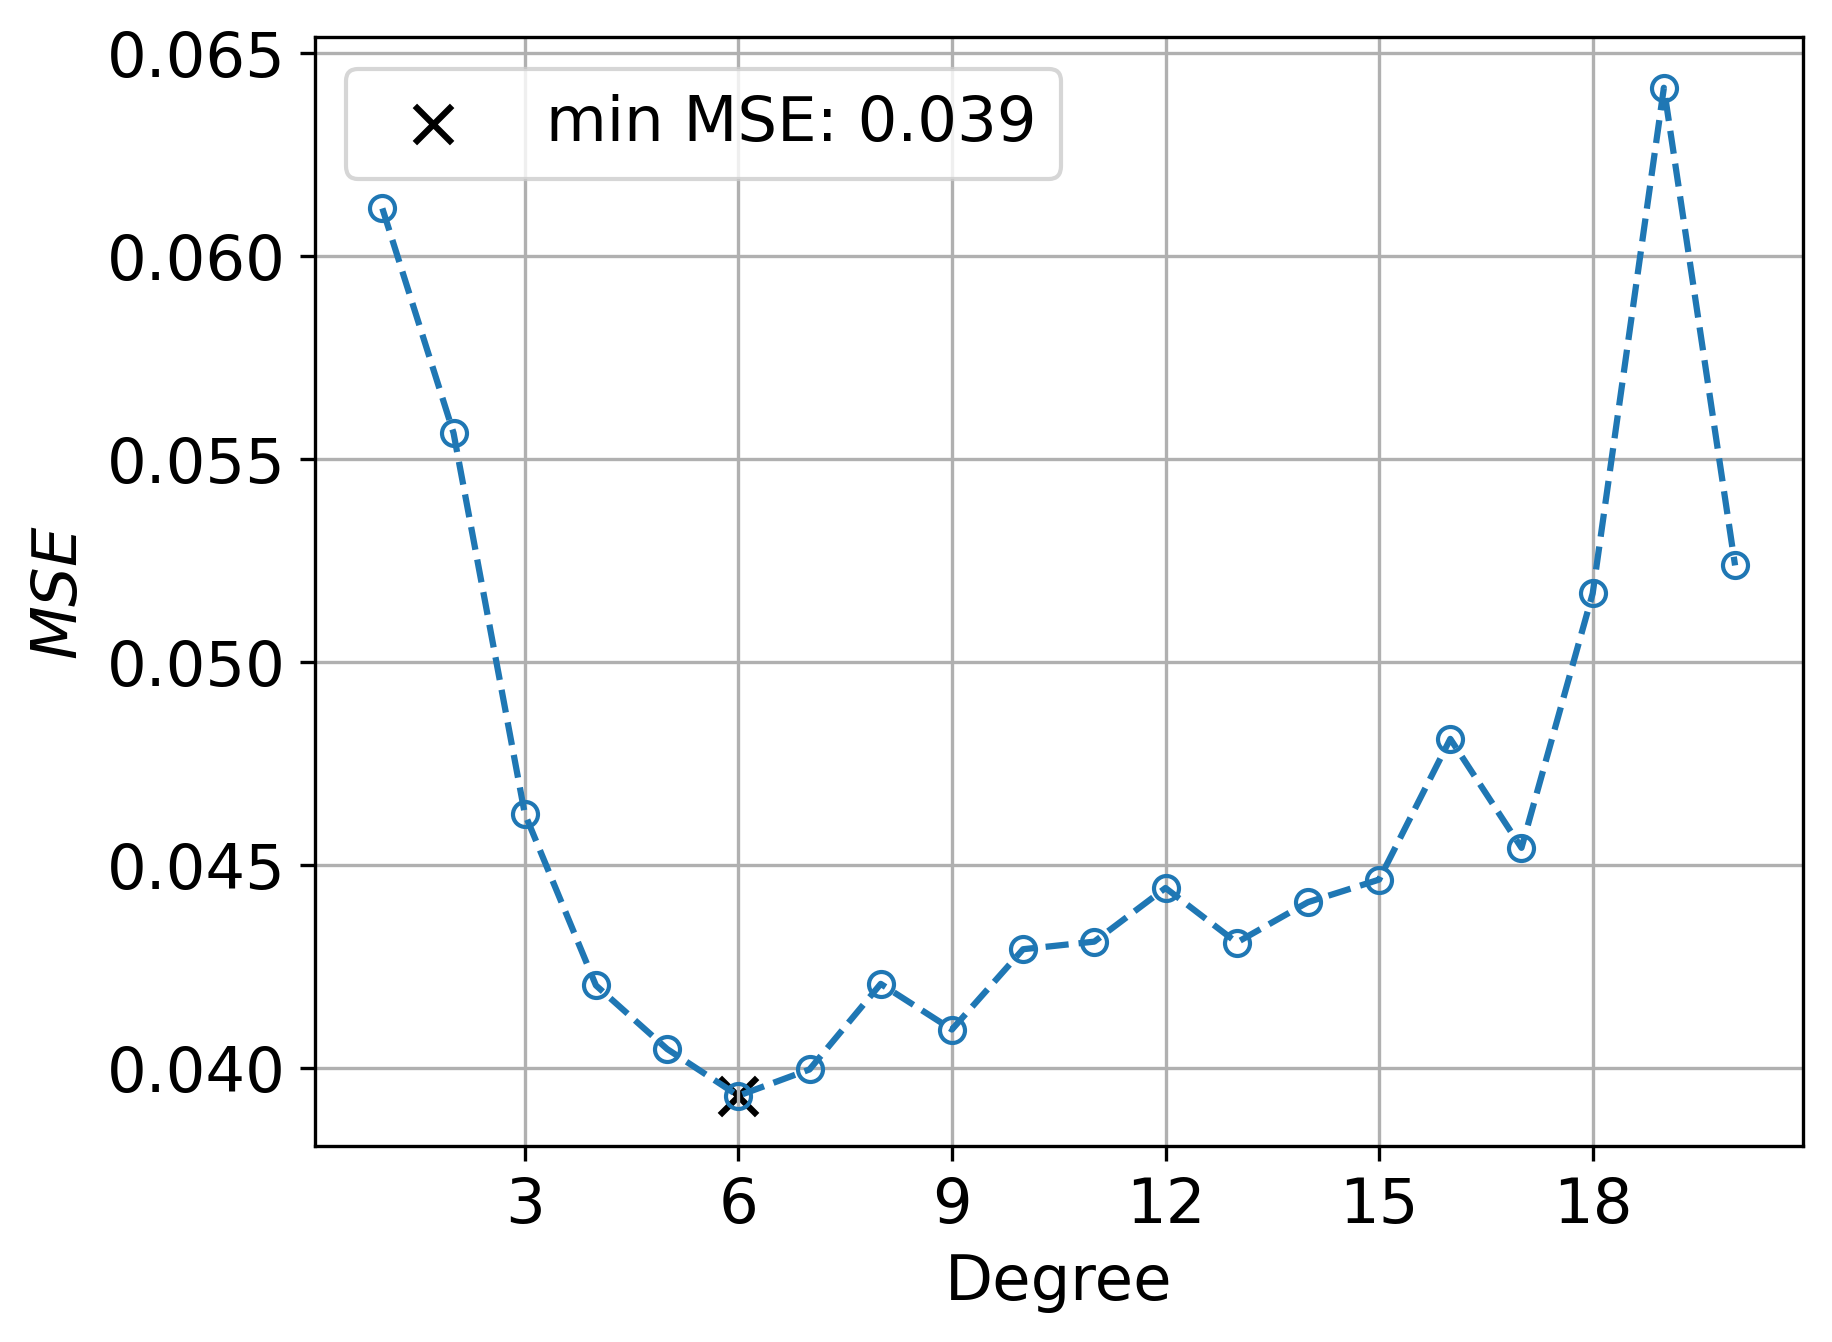
\includegraphics[width=.7\textwidth]{../figures/best_lambda_OLS_02_franke.png}
  \caption{Cross validation to find which polynomial degree gives the lowest MSE for data with $n=30$ steps and noise standard deviation $\sigma=0.2$}
  \label{fig:best_OLS}
\end{figure}

\begin{figure}[H]

  \begin{subfigure}{.5\textwidth}
    \centering
    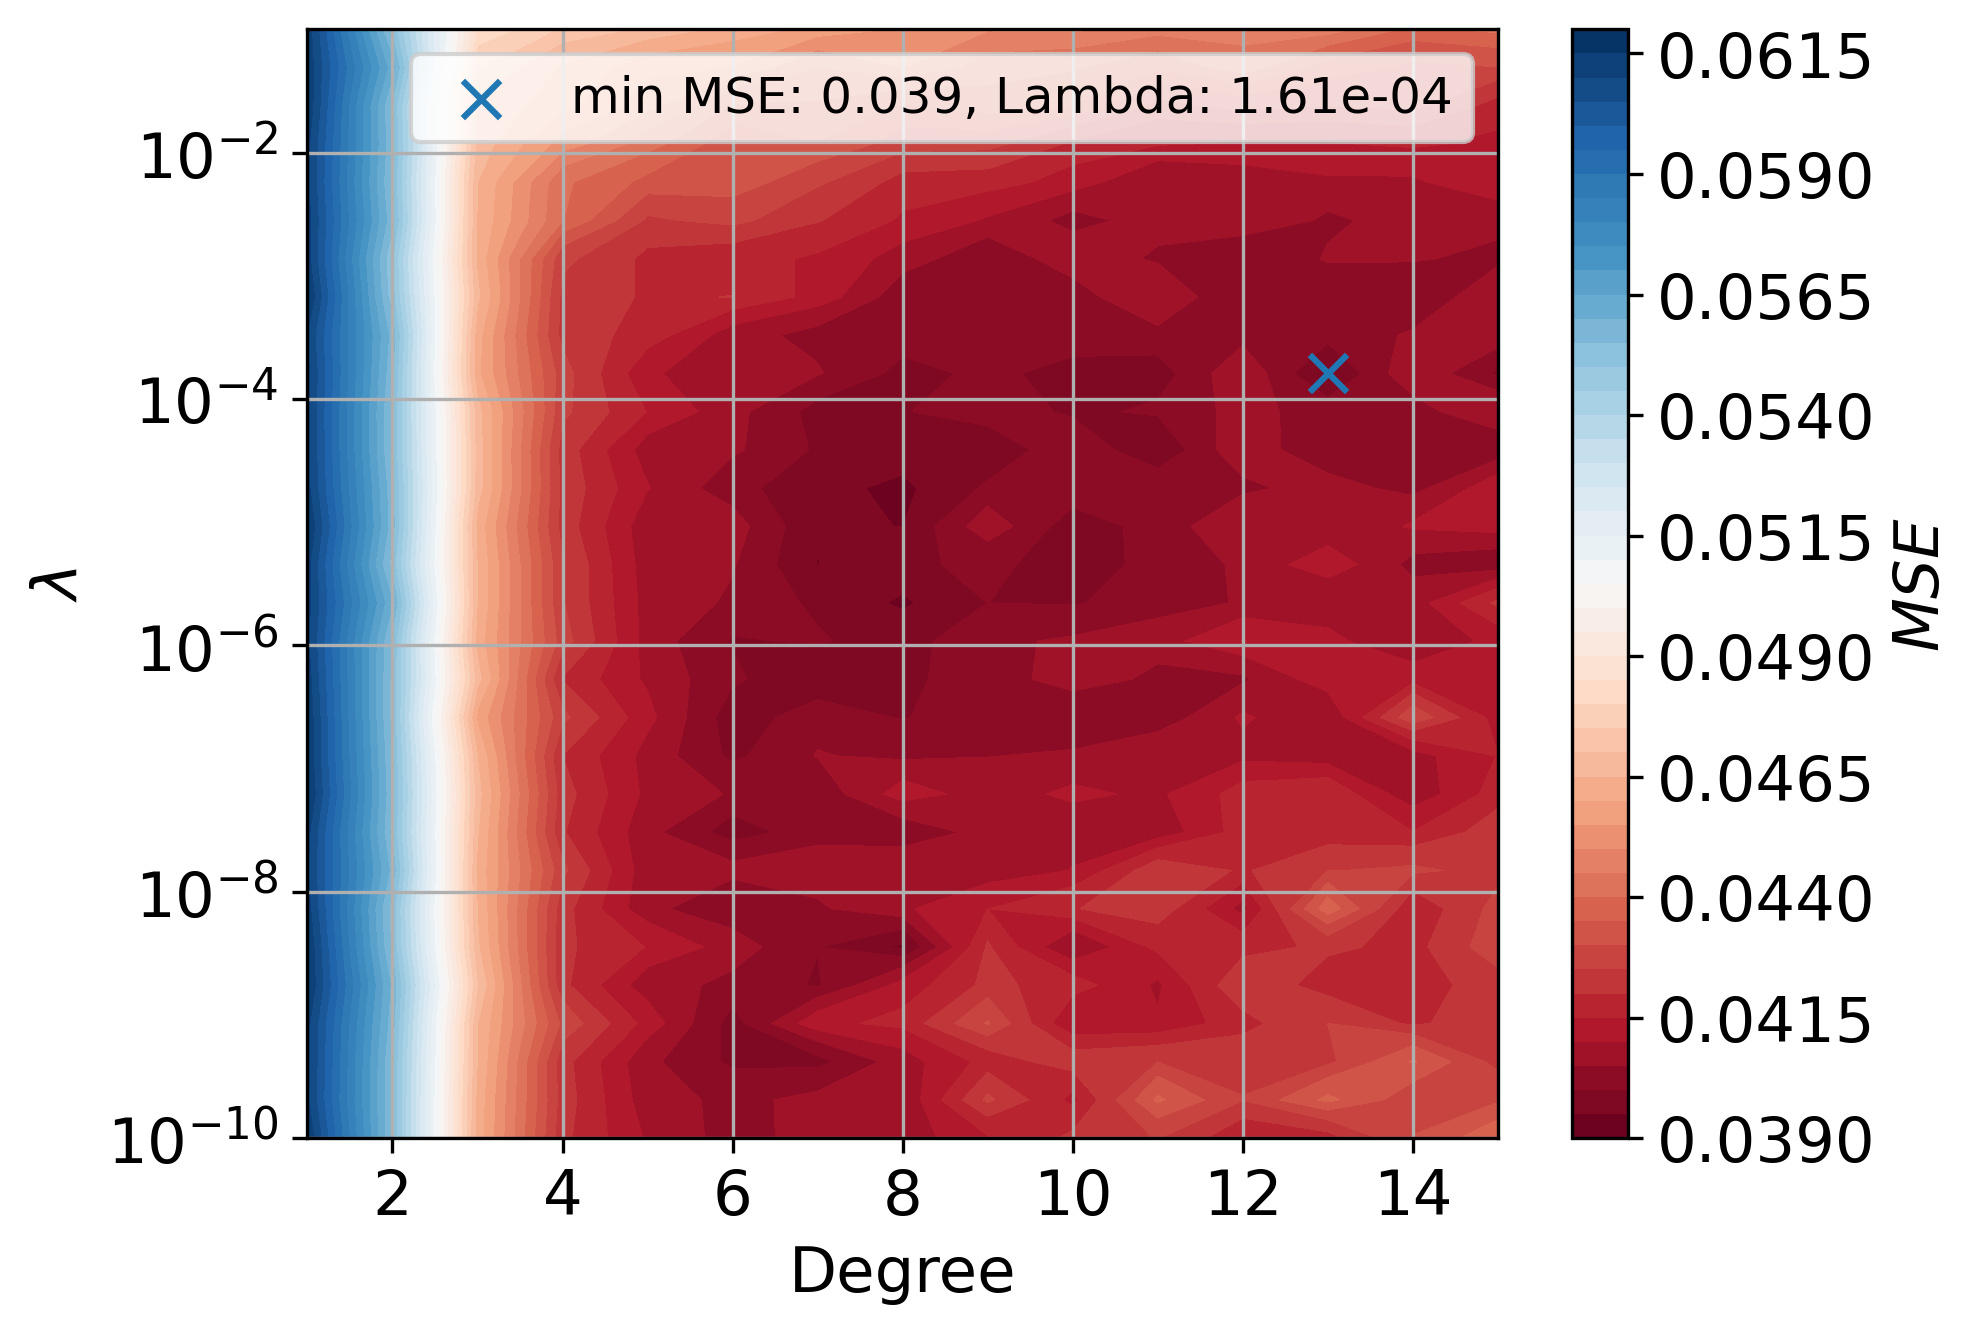
\includegraphics[width=\textwidth]{../figures/best_lambda_RIDGE_02.png}
    \caption{Ridge regression}
    \label{fig:}
  \end{subfigure}
  \begin{subfigure}{.5\textwidth}
    \centering
    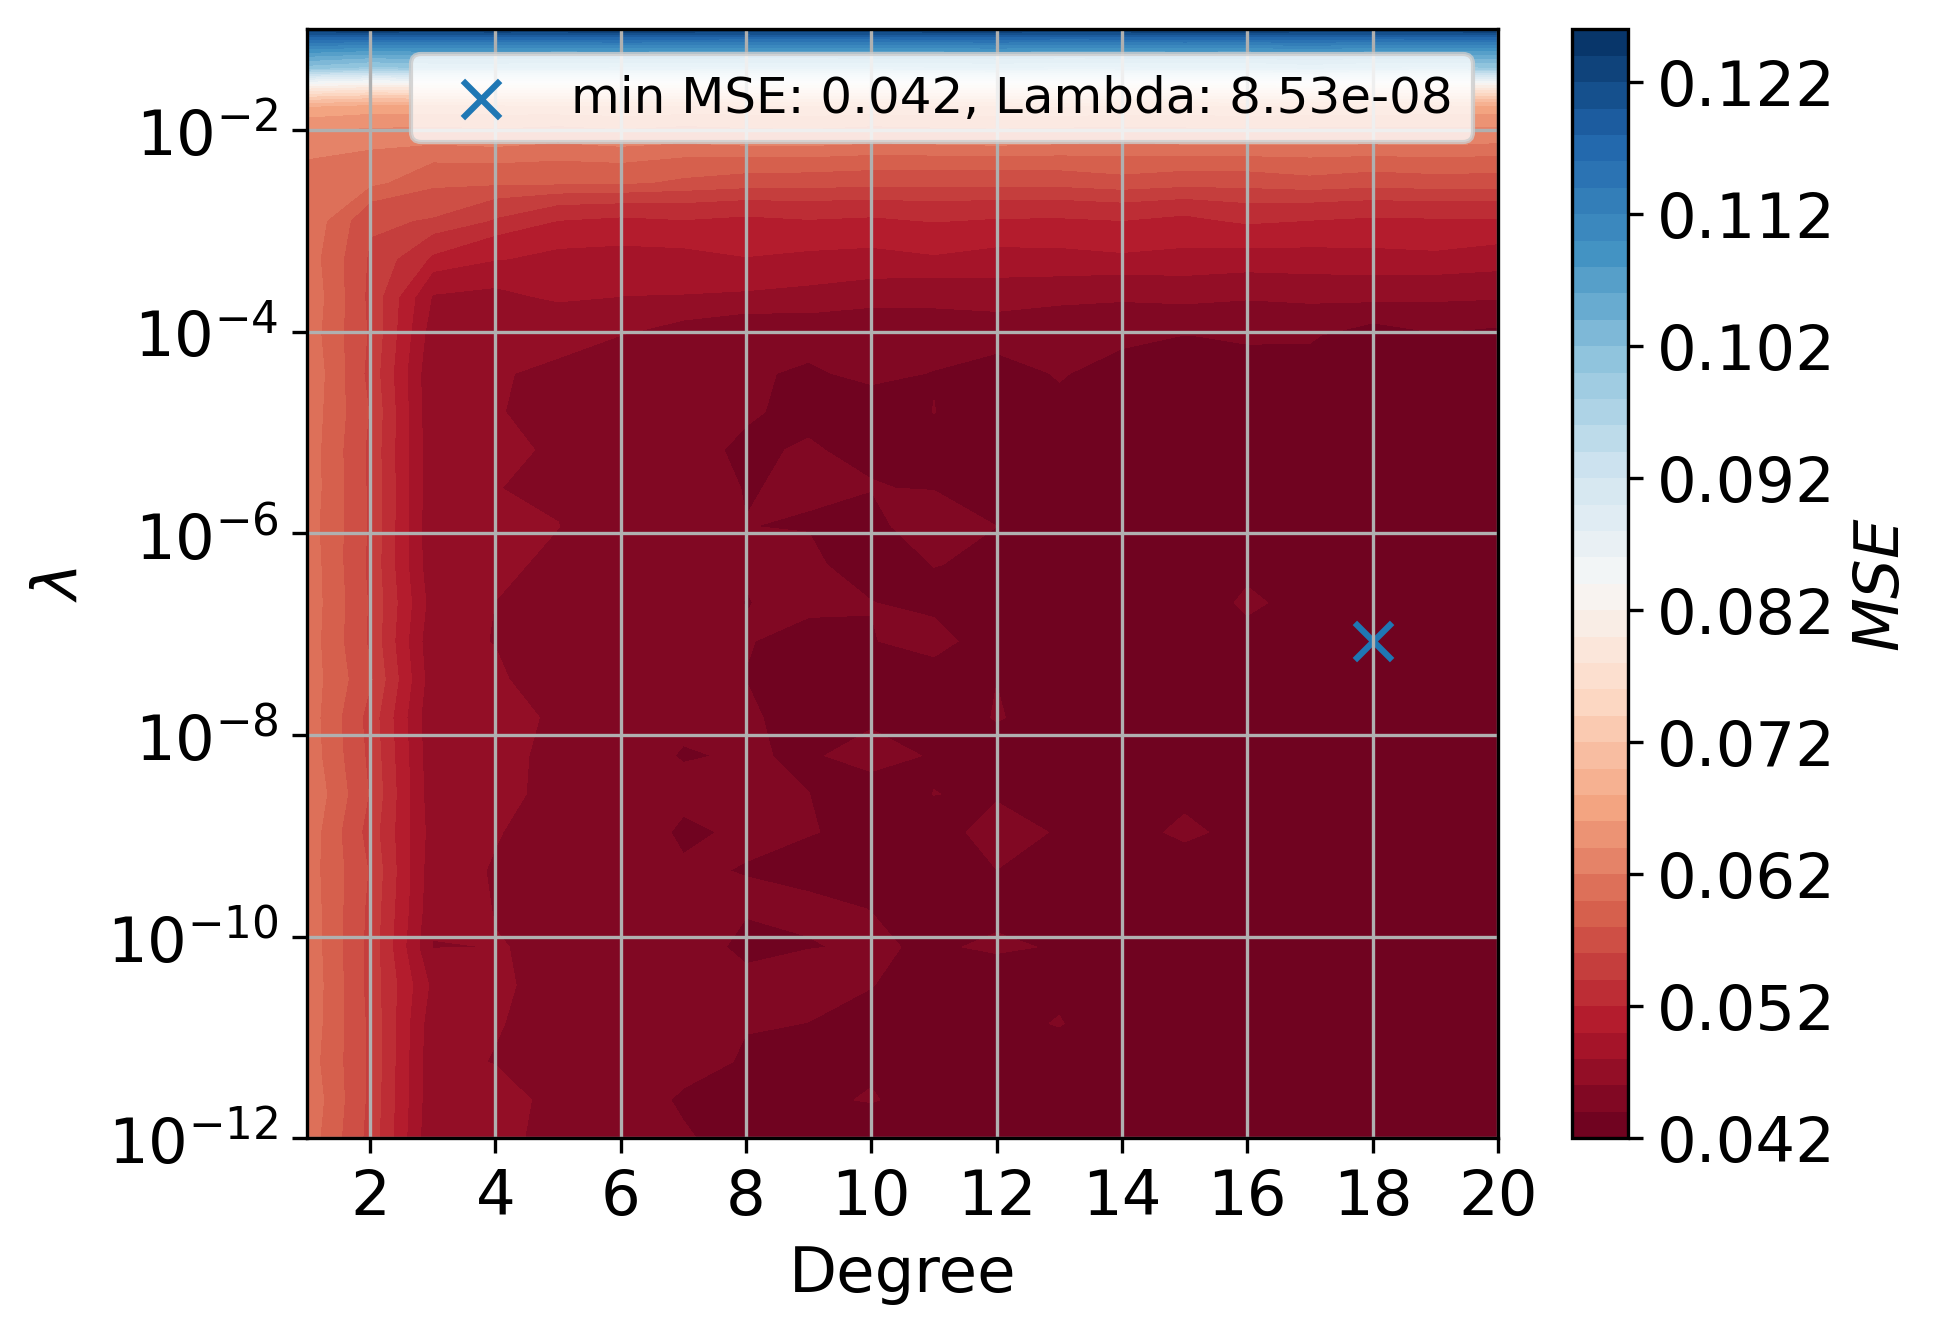
\includegraphics[width=\textwidth]{../figures/best_lambda_LASSO_02.png}
    \caption{Lasso regression}
    \label{fig:}
  \end{subfigure}
  \caption{Heatmap of MSE for different choices of polynomial degree and $\lambda$. Here we have used cross validation with 5$k$-folds for data with $n=30$ steps and noise standard deviation of $\sigma=0.2$}
  \label{fig:heat_franke}
\end{figure}

Above in figure \ref{fig:best_OLS} we see similar to figure \ref{fig:cv_comp} that we for a degree of 6 minimize the MSE for OLS regression. This means that if we want to compute the best possible prediction $\tilde{z}$ we should use a design matrix of degree 6.

For Ridge and Lasso in figure \ref{fig:heat_franke} we see a clear dependency on both $\lambda$ and polynomial degree. Ridge reaches lower MSE for lower degrees than lasso which needs to be plotted up to a degree of 20 to find an optimal degree of 18. MSE in the ridge plot is variating more when changing $\lambda$ than what we see for the lasso method which mostly only changes down to a $\lambda$ of $10^{-4}$. This corresponds to what we saw in the bias variance tradeoff in figure \ref{fig:ridge_tradeoff} and \ref{fig:lasso_tradeoff} where we saw almost no change in the lasso tradeoff for changes to $\lambda$ parameters smaller than $10^{-4}$. In total, this together with figure \ref{fig:best_OLS} have given us a way of finding which model gives the most optimal results. This is shown in table \ref{tab:best_comp}.
\begin{table}[H]
  \centering
  \caption{Table of best parameters and the following MSE for OLS, Ridge and Lasso regression}
  \label{tab:best_comp}
  \begin{tabular}{|c||c|c|c|}
    \hline
    Method & $\lambda$ & Degree & $MSE$ \\
    \hline
    OLS &  & 6 & 0.0393 \\
    \hline
    RIDGE & $1.61\times10^{-7}$ & 8 & 0.0390 \\
    \hline
    LASSO & $8.53\times10^{-8}$ & 19 & 0.0424 \\
    \hline
  \end{tabular}
\end{table}
We see from table \ref{tab:best_comp} very close results, especially between OLS and Ridge regression. Ridge barely beats OLS with a slightly lower MSE while Lasso is still a bit behind them both.

\subsubsection{Prediction plots}
We use the results from table \ref{tab:best_comp} to show the predictions of our models in figure \ref{fig:pred_franke} on the next page. To also gain a better visual understanding on how our regression methods perform with the chosen parameters from table \ref{tab:best_comp}, we also perform a new training and prediction just with a greater data sample of $n=200$ steps in figure \ref{fig:extra_pred_franke}.
\begin{figure}[H]
  \begin{subfigure}{.5\textwidth}
    \centering
    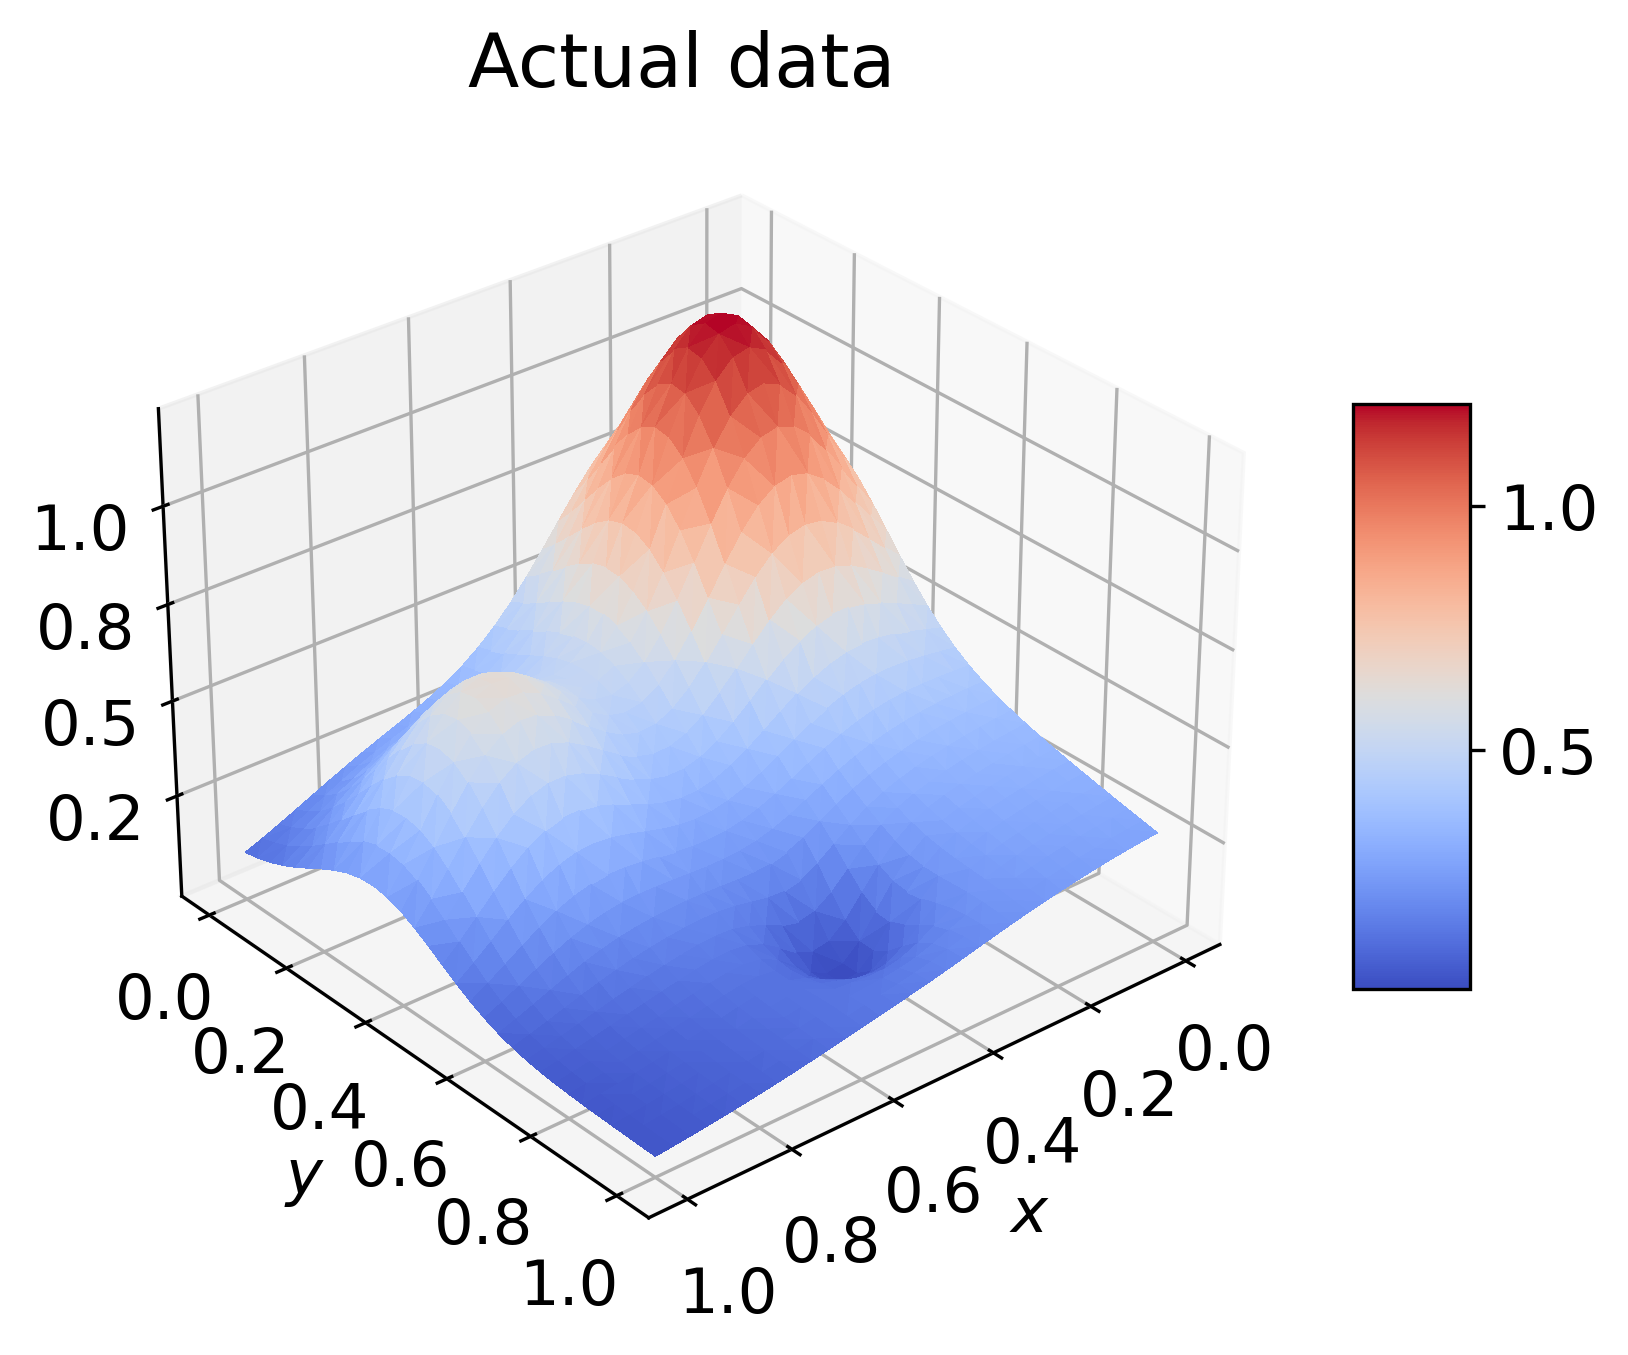
\includegraphics[width=\textwidth]{../figures/actual_data_franke_2.png}
    \caption{Franke function}
    \label{fig:pred_real}
  \end{subfigure}
  \begin{subfigure}{.5\textwidth}
    \centering
    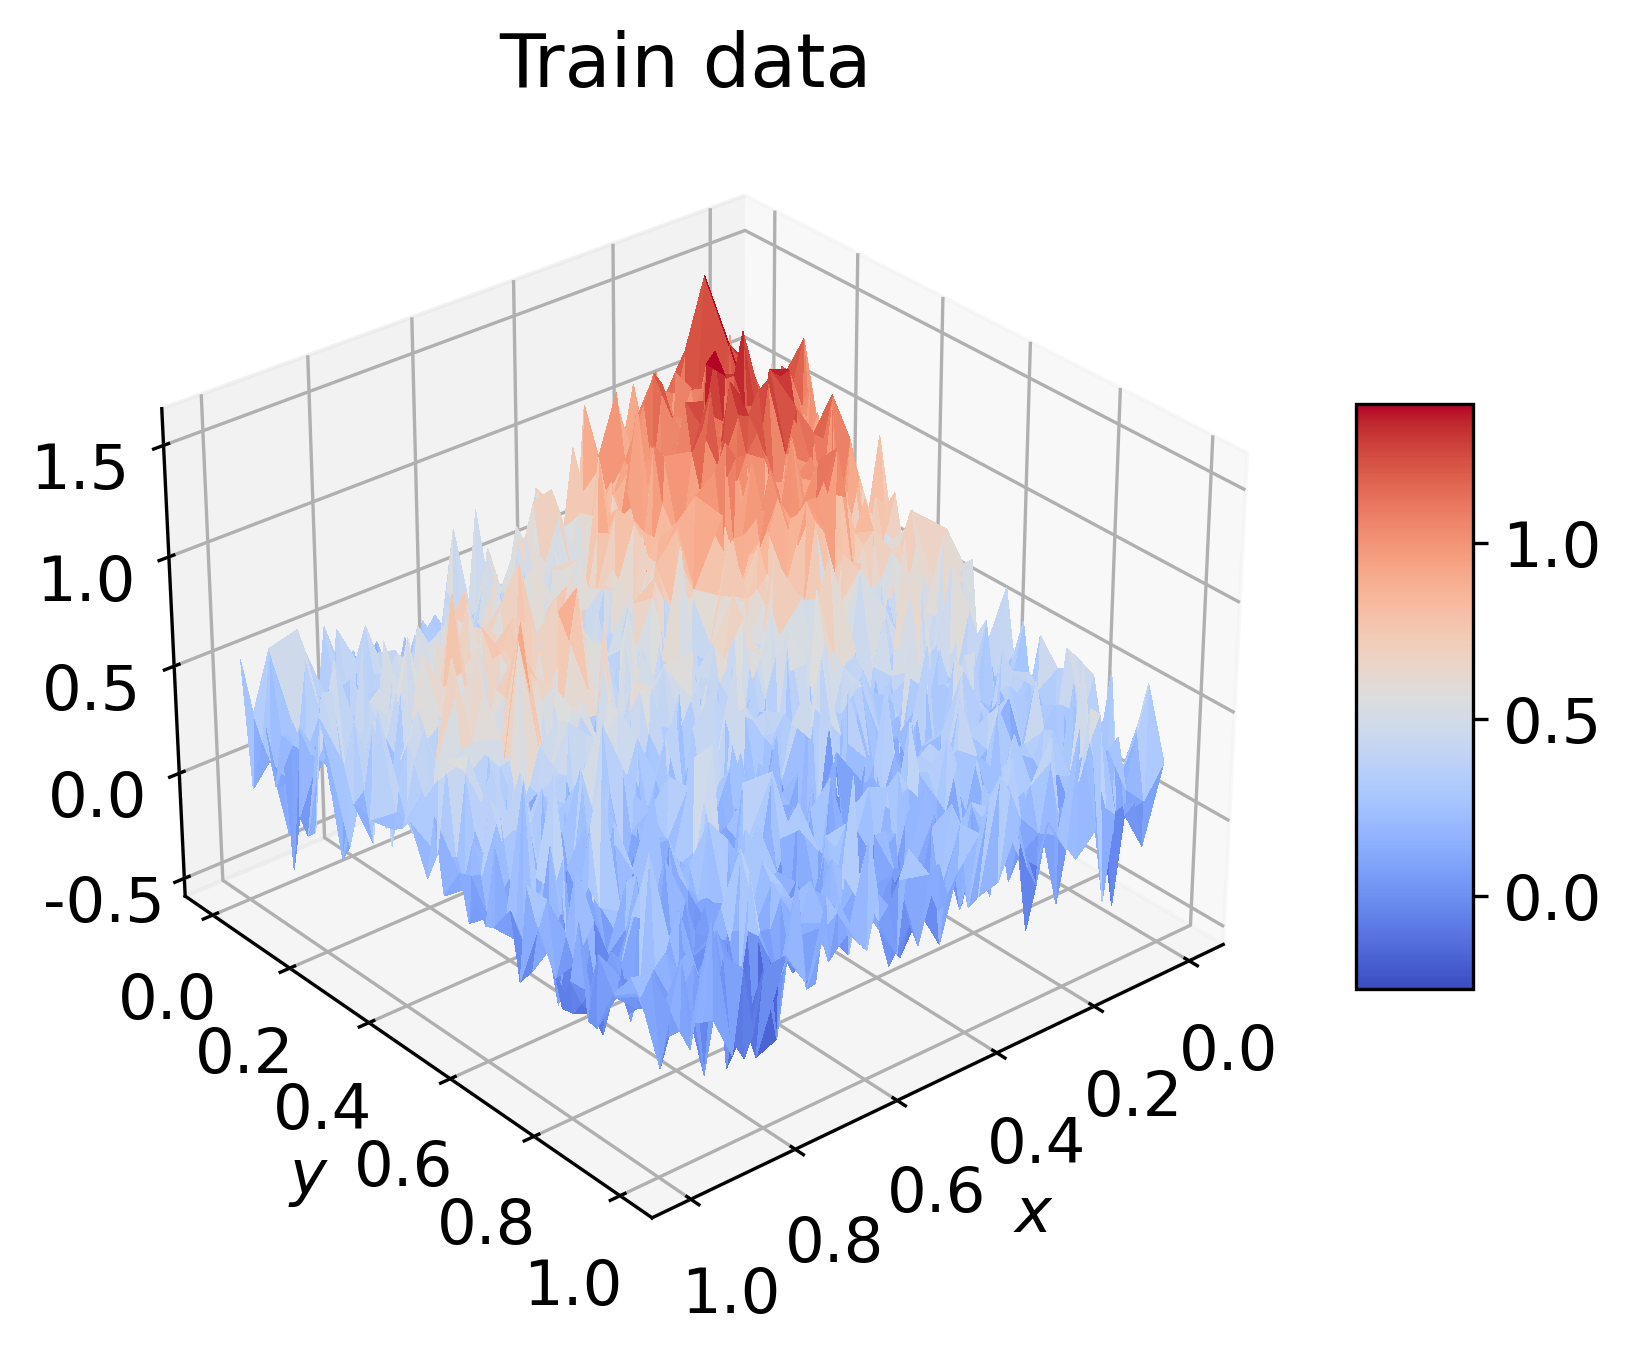
\includegraphics[width=\textwidth]{../figures/train_data_franke_2.png}
    \caption{Train data from function data with added noise}
    \label{fig:pred_train}
  \end{subfigure}
  \begin{subfigure}{.5\textwidth}
    \centering
    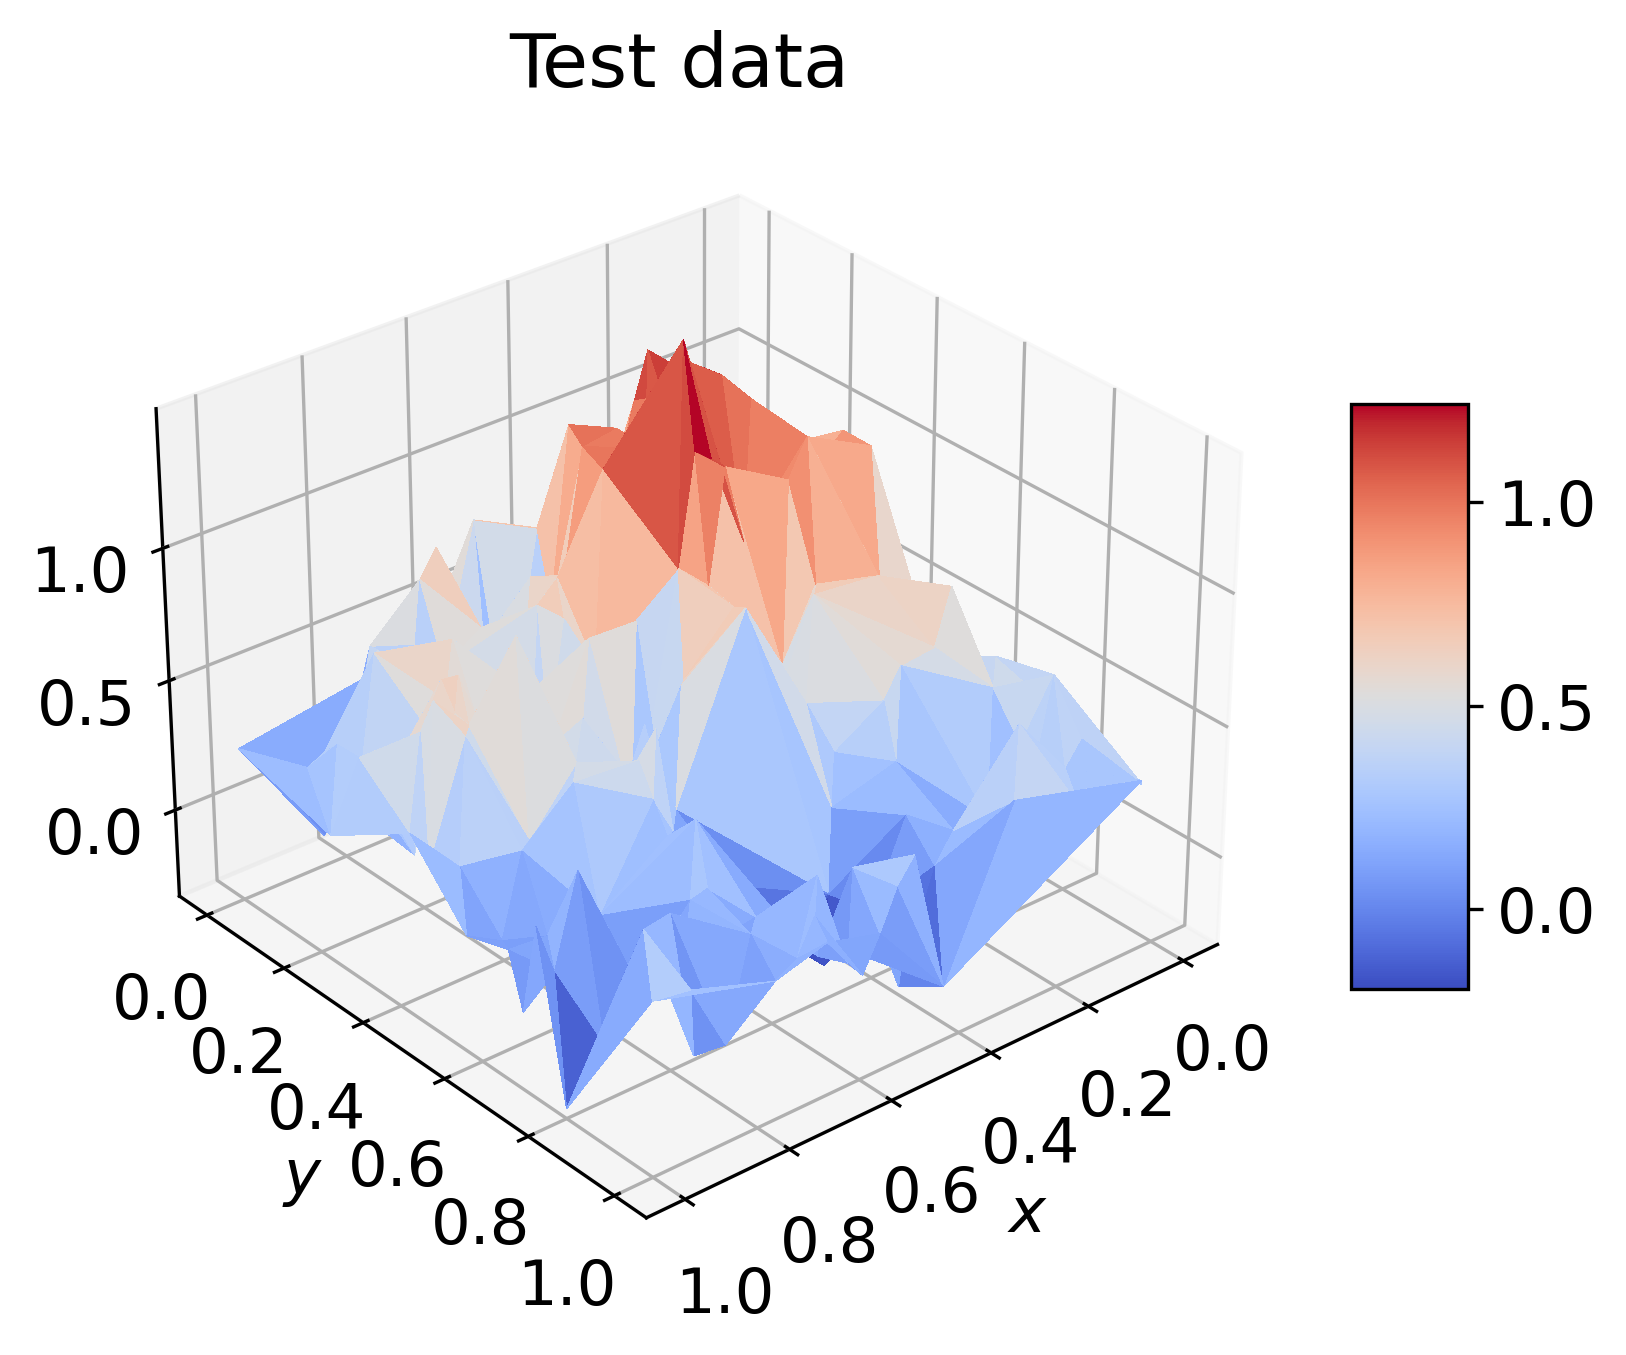
\includegraphics[width=\textwidth]{../figures/test_data_franke_2.png}
    \caption{Test data from function data with added noise}
    \label{fig:pred_test}
  \end{subfigure}
  \begin{subfigure}{.5\textwidth}
    \centering
    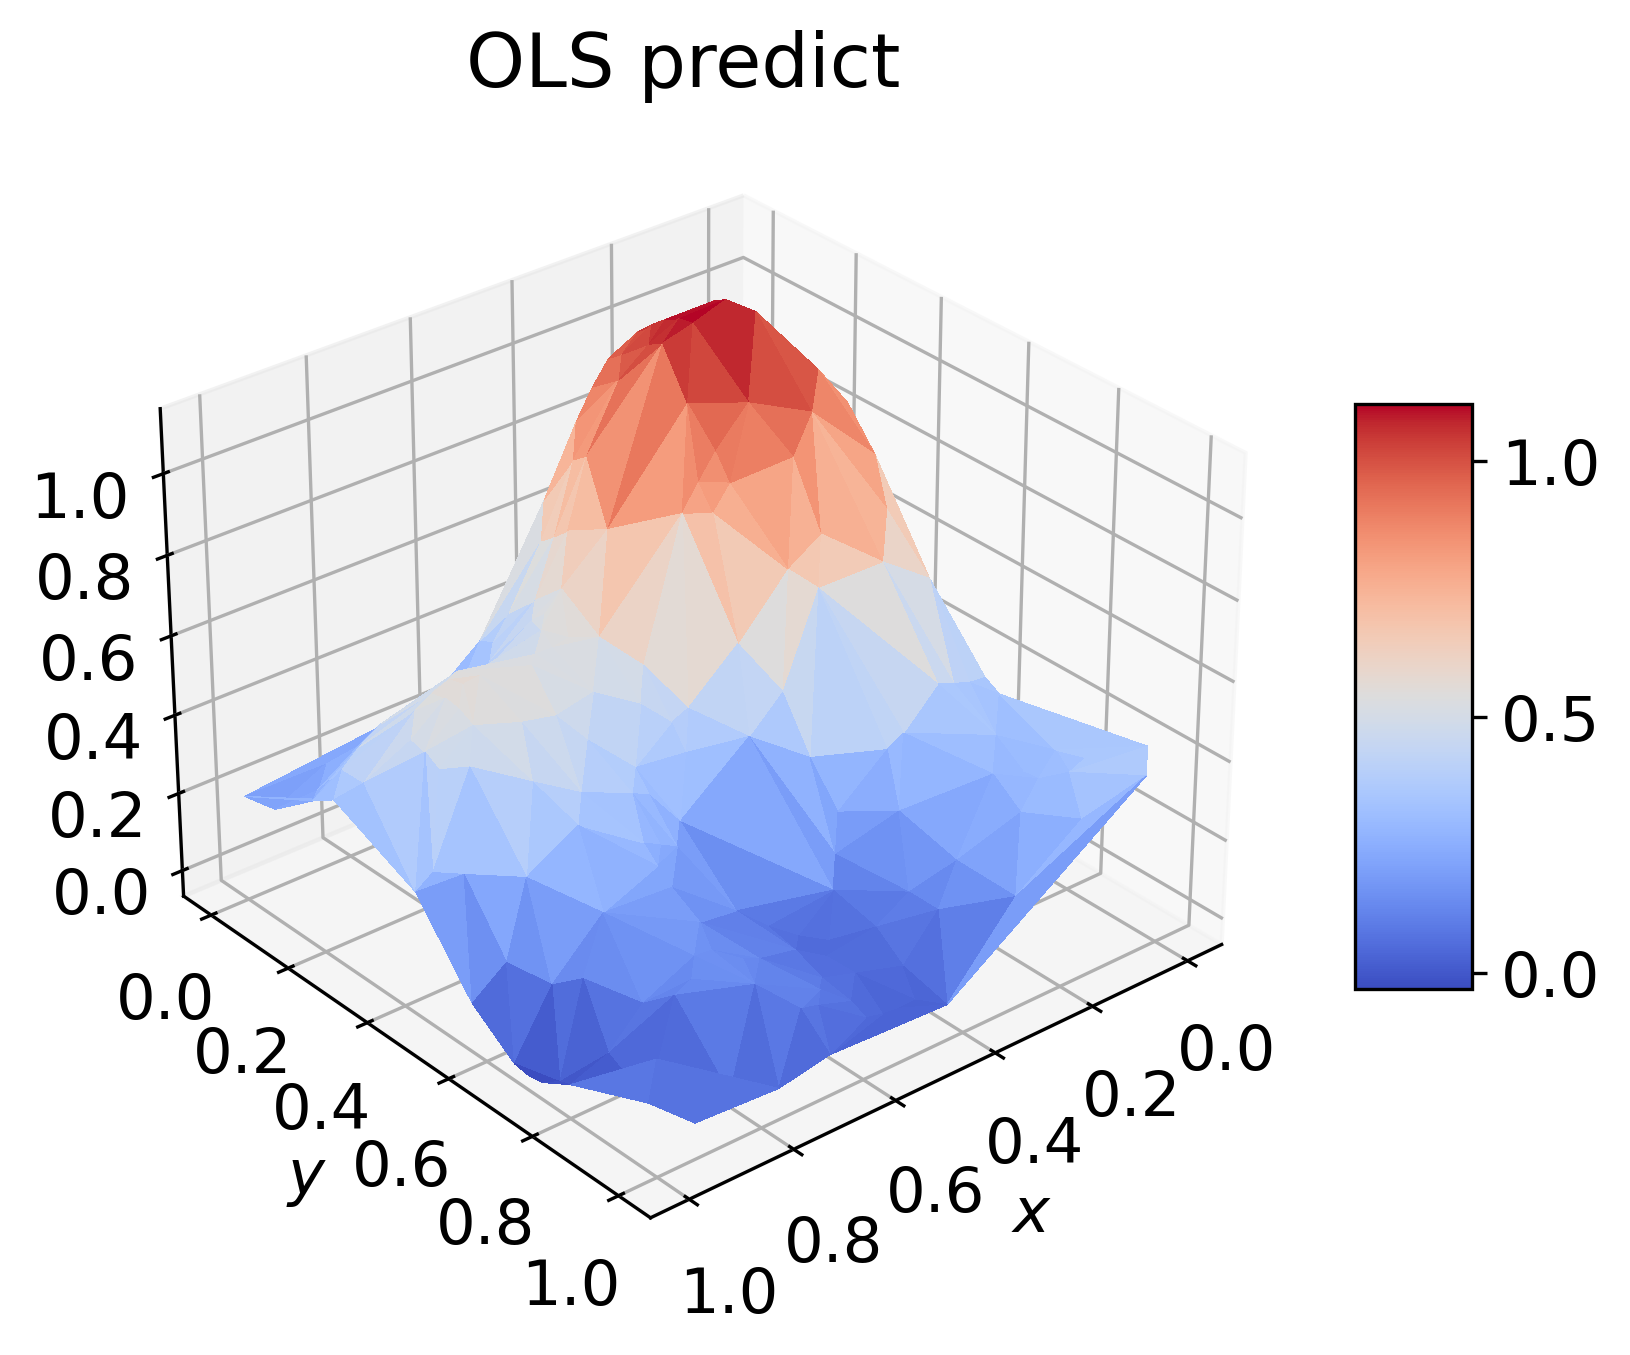
\includegraphics[width=\textwidth]{../figures/ols_pred_franke_2.png}
    \caption{OLS prediction}
    \label{fig:pred_ols}
  \end{subfigure}
  \begin{subfigure}{.5\textwidth}
    \centering
    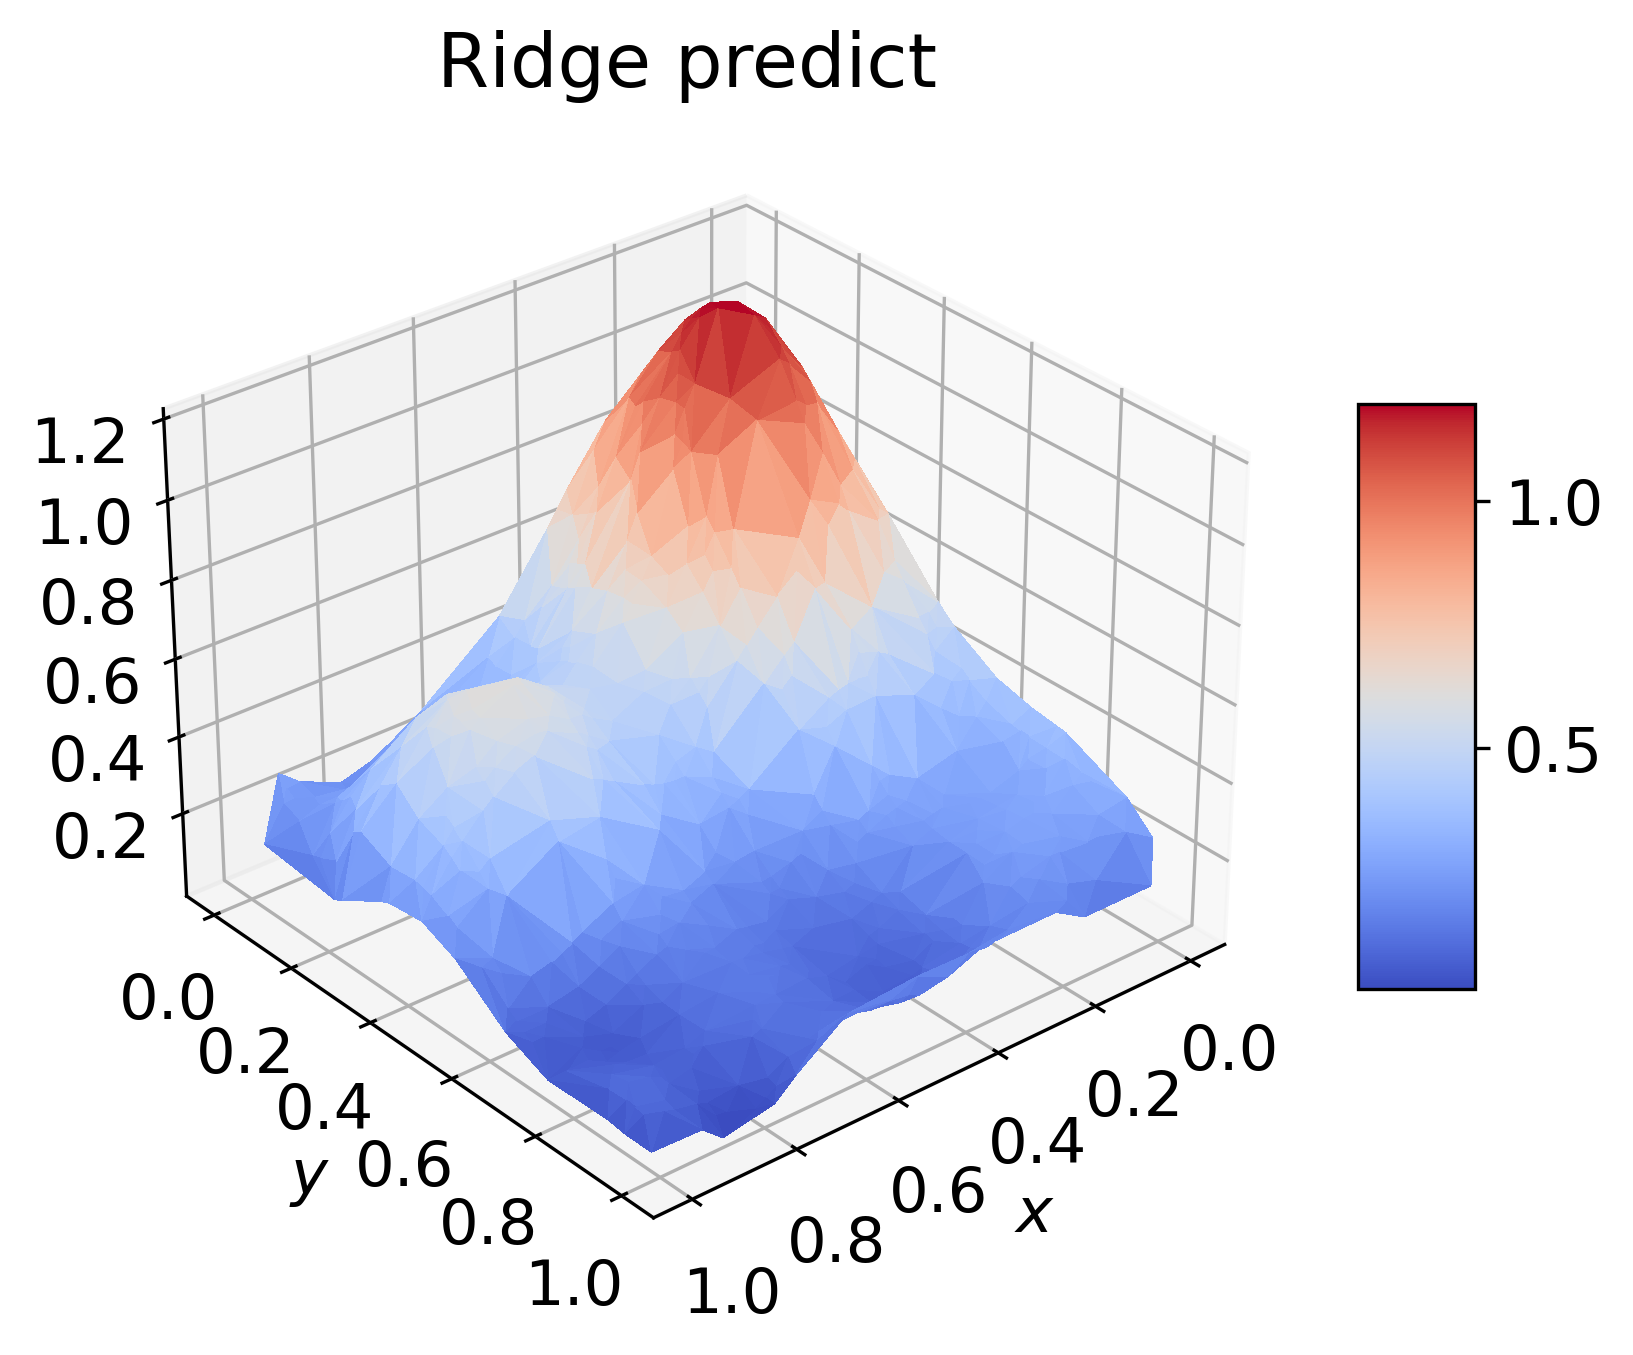
\includegraphics[width=\textwidth]{../figures/ridge_pred_franke_2.png}
    \caption{Ridge prediction}
    \label{fig:pred_ridge}
  \end{subfigure}
  \begin{subfigure}{.5\textwidth}
    \centering
    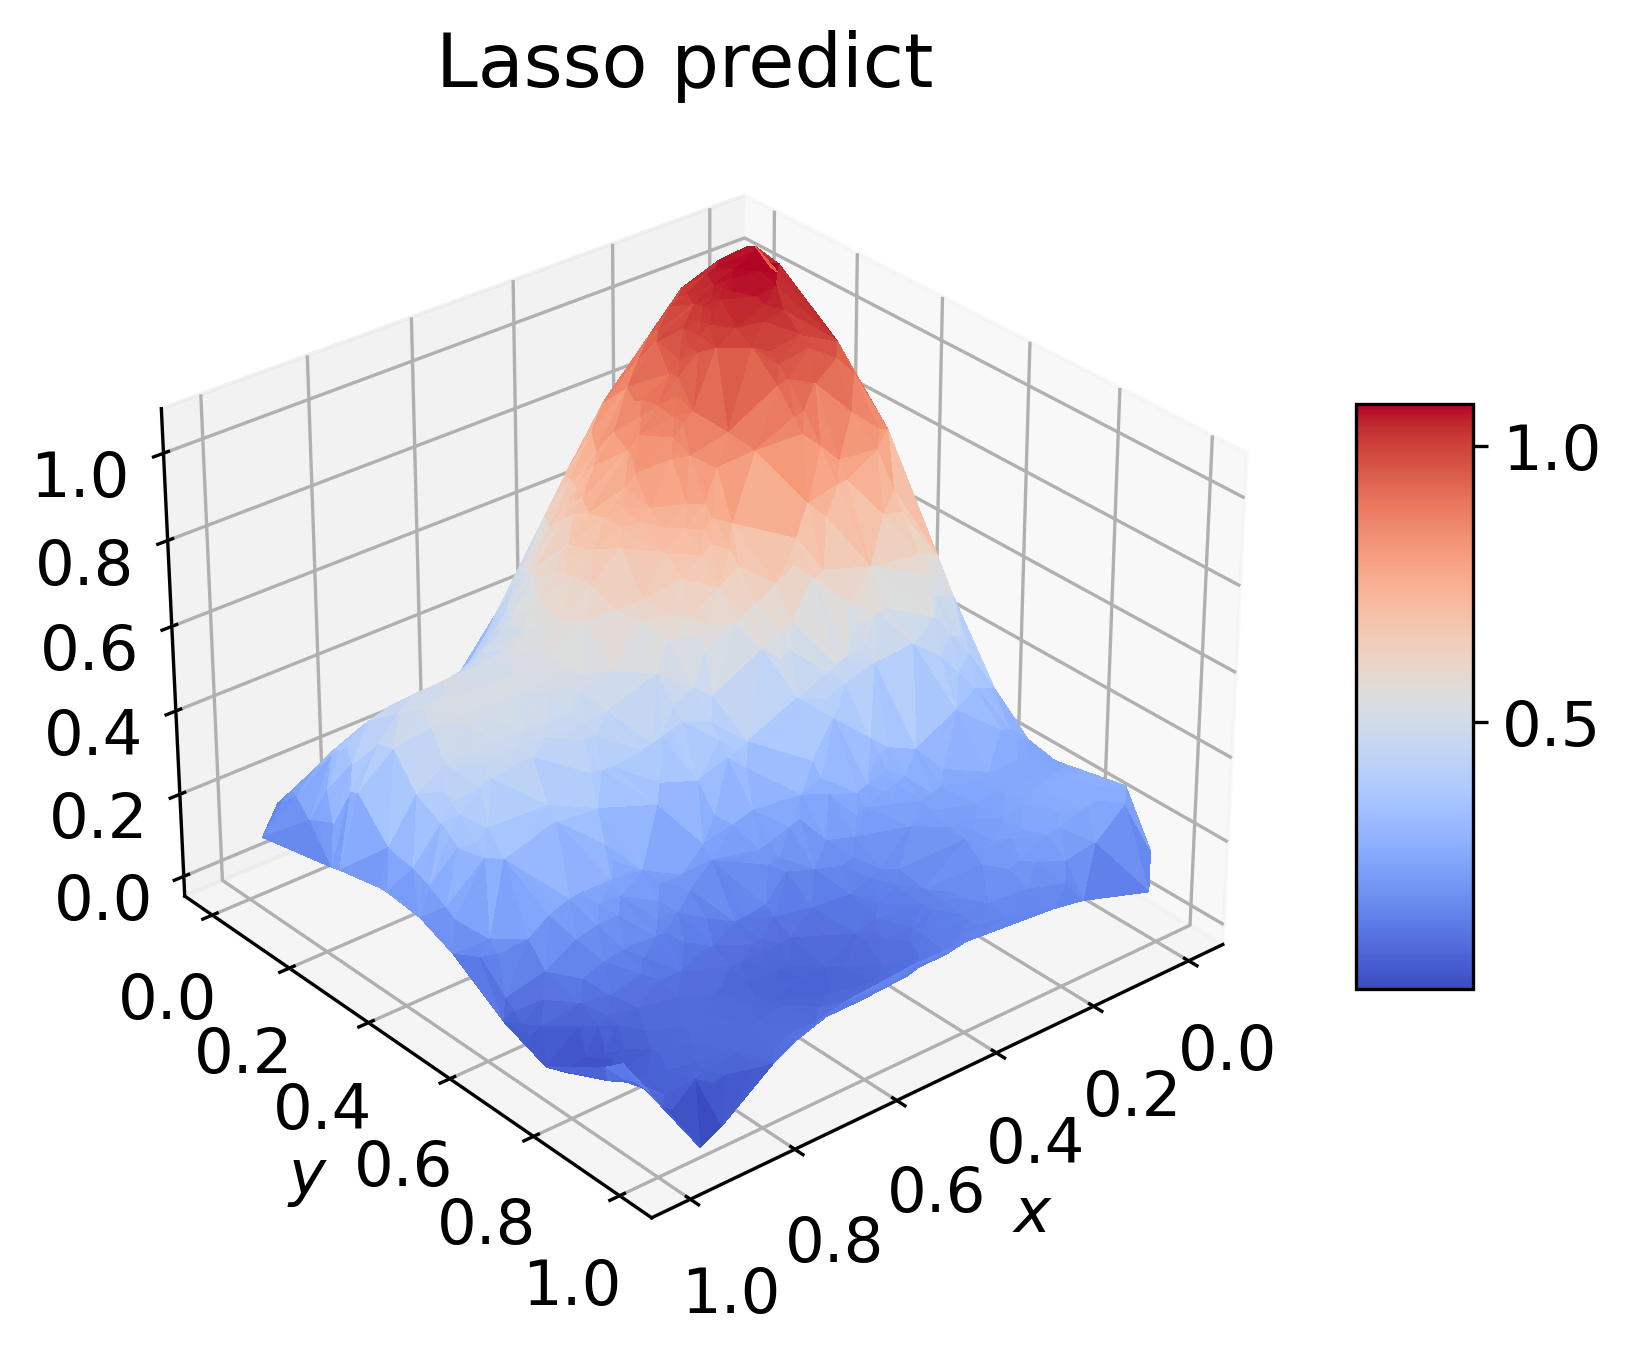
\includegraphics[width=\textwidth]{../figures/lasso_pred_franke_2.png}
    \caption{Lasso prediction}
    \label{fig:pred_lasso}
  \end{subfigure}
  \caption{Plot of the true Franke function together with our train and test data, and our predictions for our optimal parameters shown in table \ref{tab:best_comp} }
  \label{fig:pred_franke}
\end{figure}


\begin{figure}[H]
  \begin{subfigure}{.5\textwidth}
    \centering
    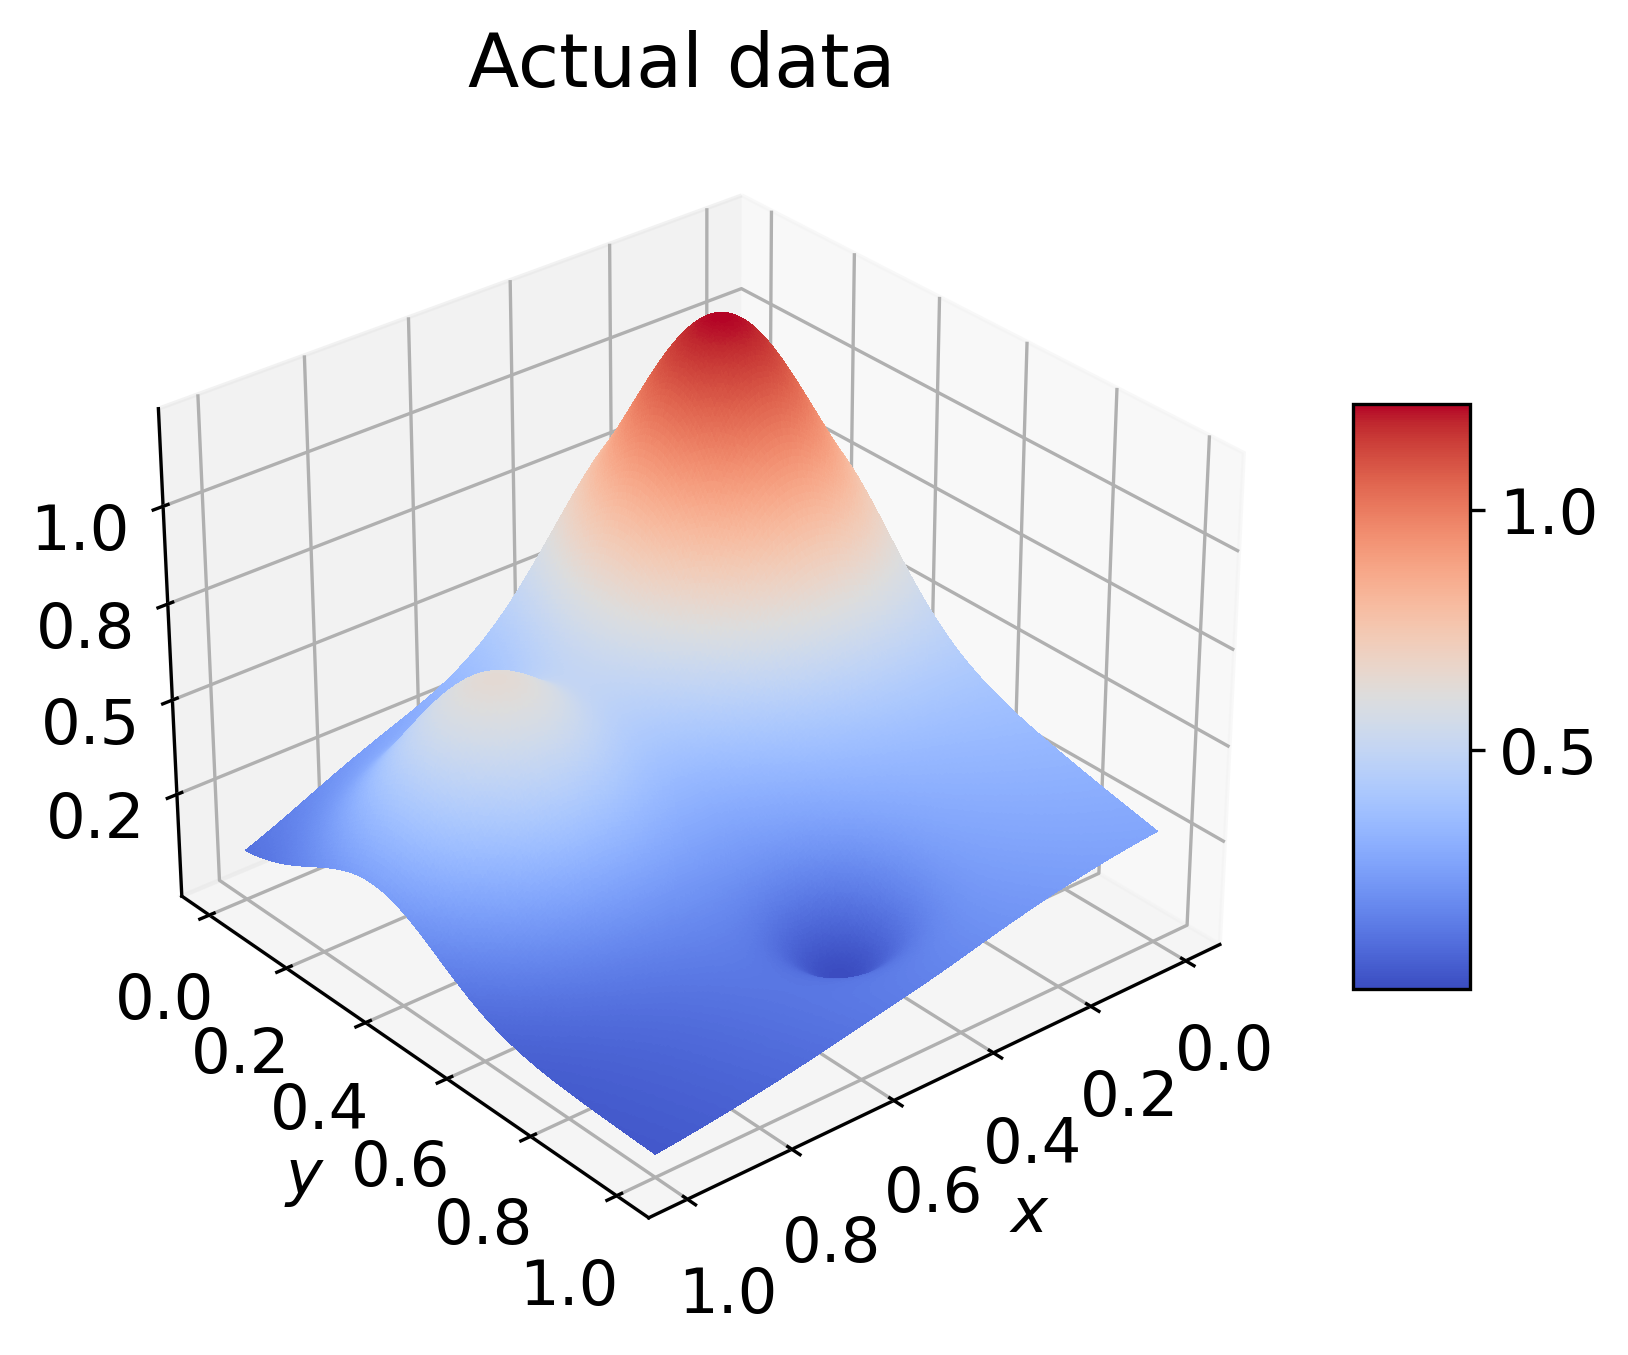
\includegraphics[width=\textwidth]{../figures/actual_data_franke_extra.png}
    \caption{Franke function}
    \label{fig:extra_pred_real}
  \end{subfigure}
  \begin{subfigure}{.5\textwidth}
    \centering
    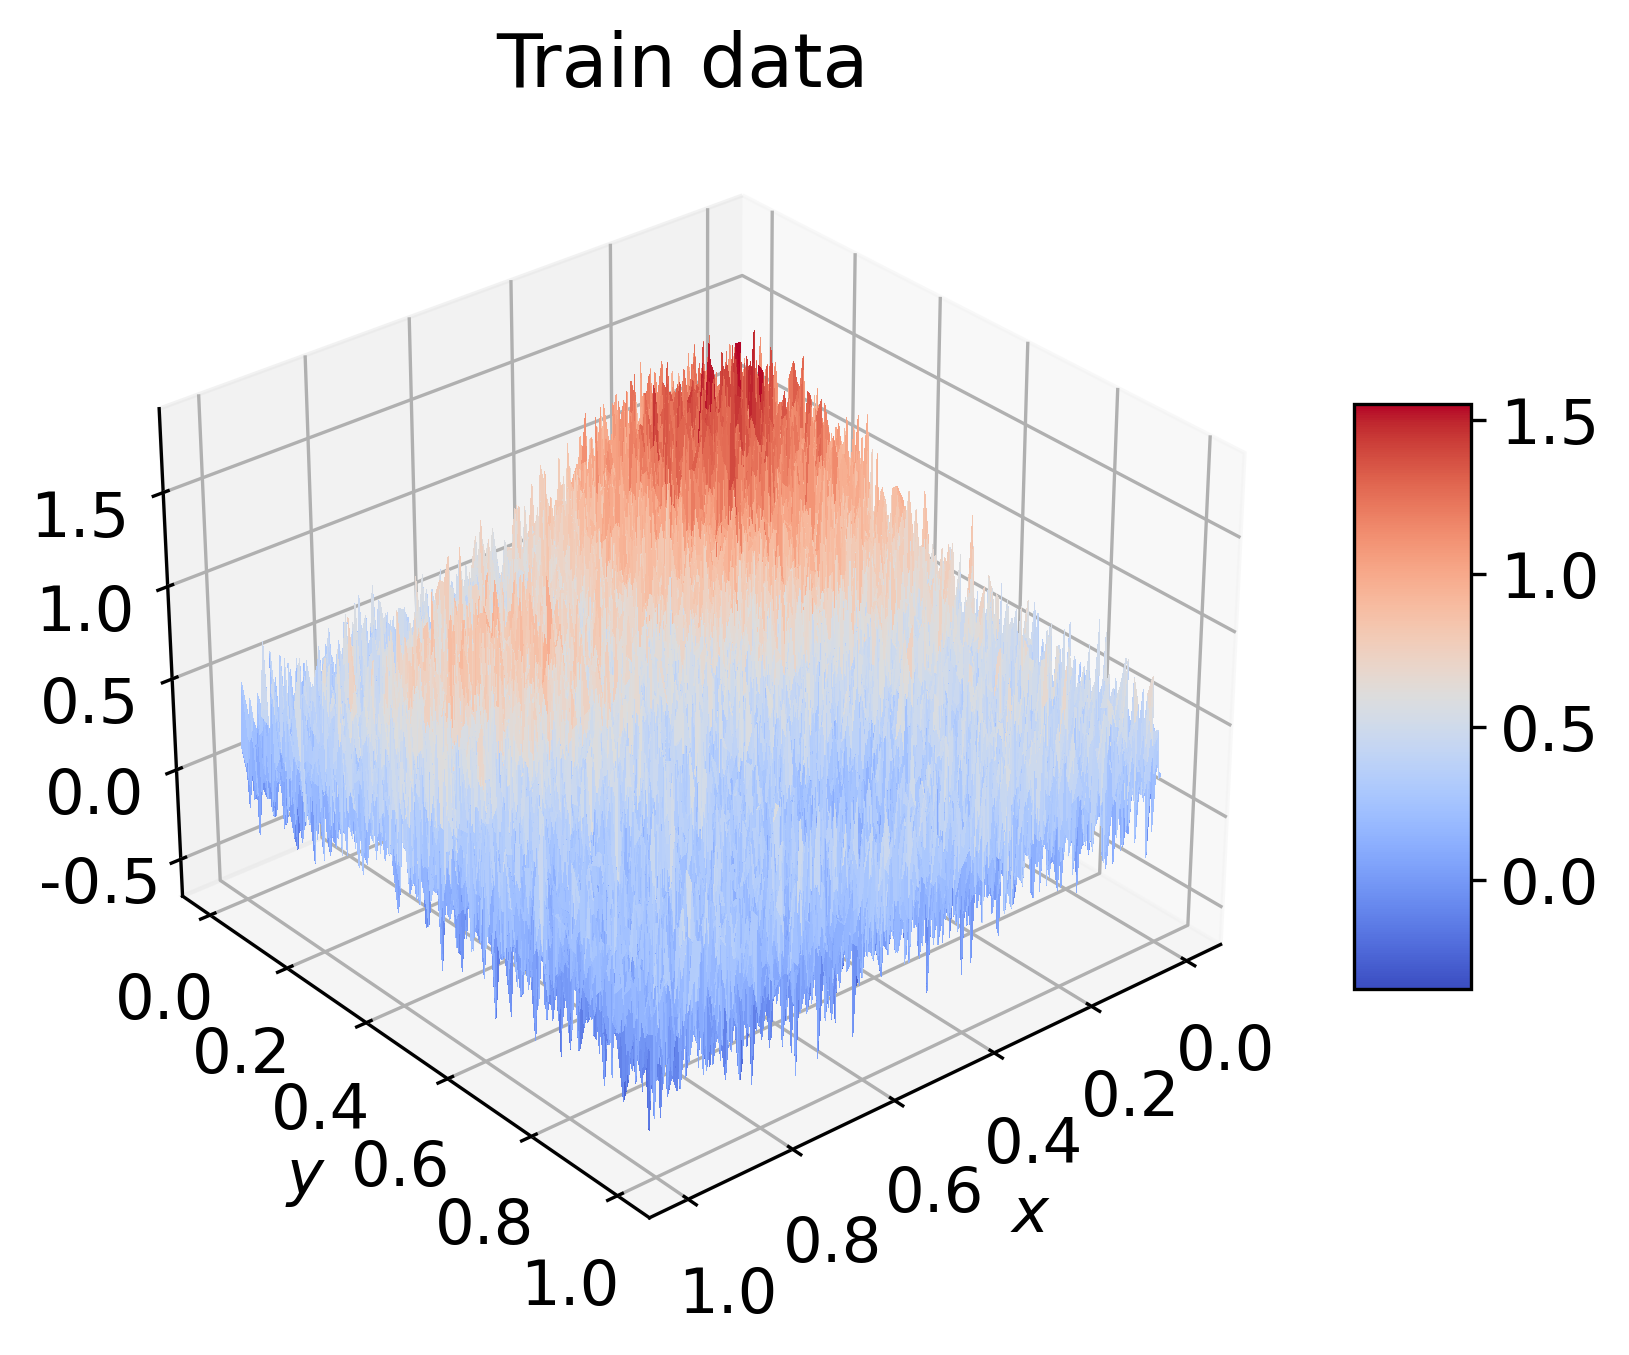
\includegraphics[width=\textwidth]{../figures/train_data_franke_extra.png}
    \caption{Train data from function data with added noise}
    \label{fig:extra_pred_train}
  \end{subfigure}
  \begin{subfigure}{.5\textwidth}
    \centering
    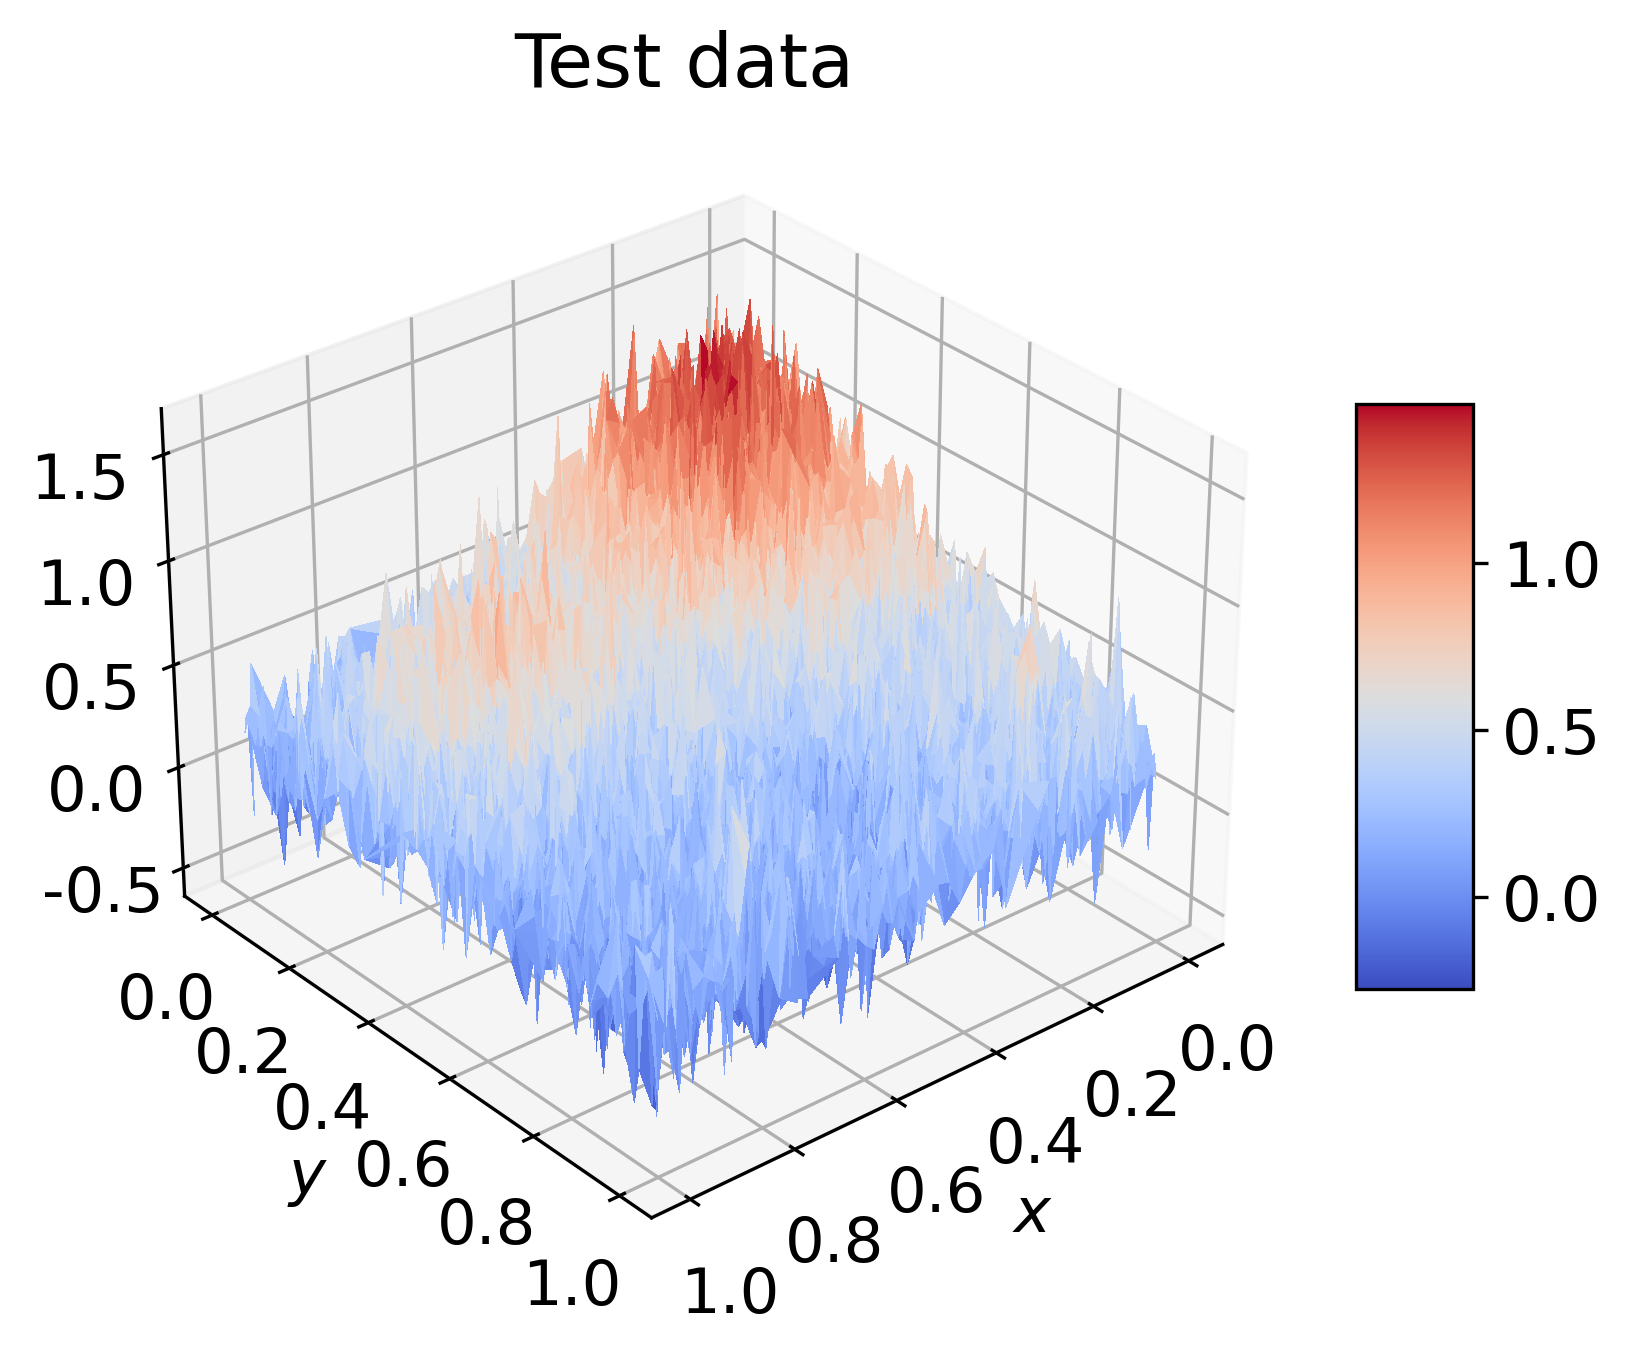
\includegraphics[width=\textwidth]{../figures/test_data_franke_extra.png}
    \caption{Test data from function data with added noise}
    \label{fig:extra_pred_test}
  \end{subfigure}
  \begin{subfigure}{.5\textwidth}
    \centering
    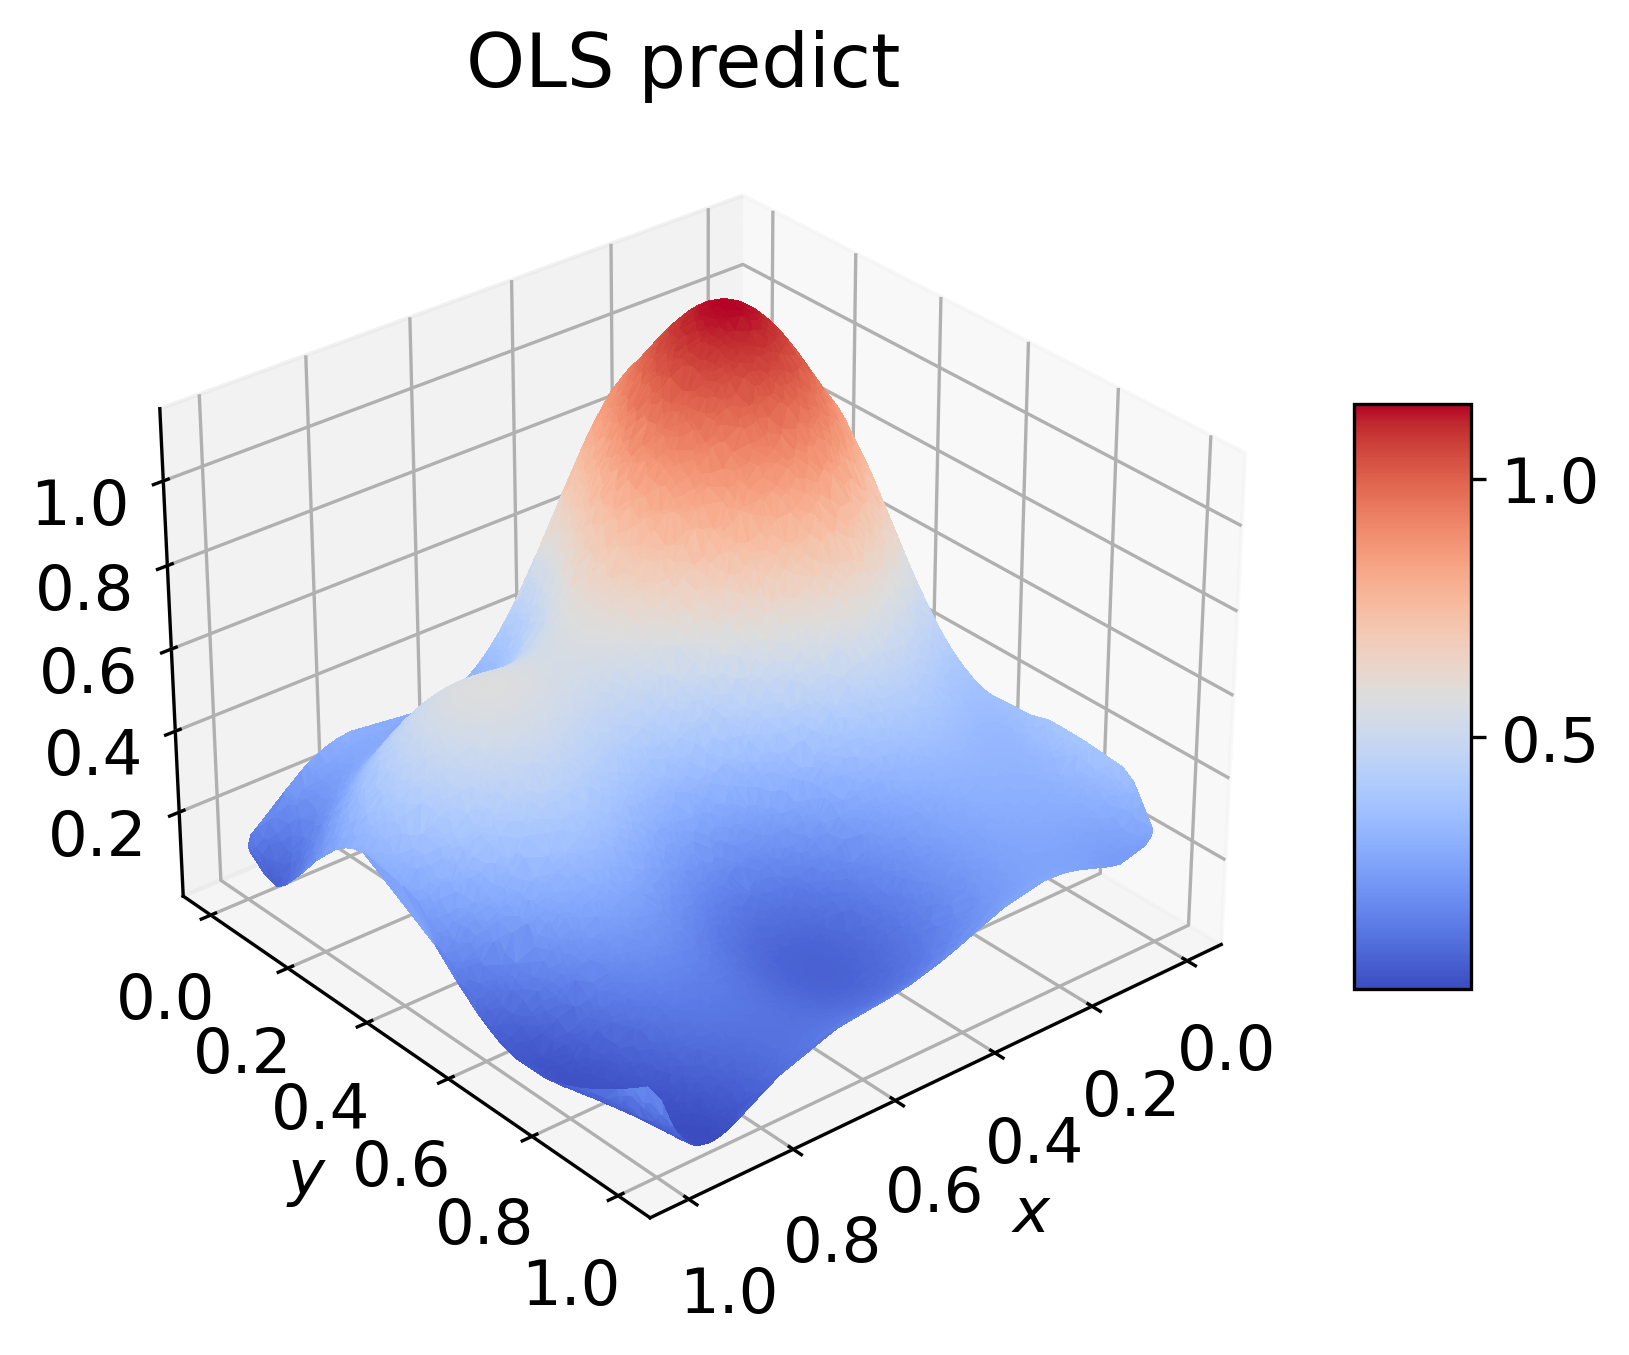
\includegraphics[width=\textwidth]{../figures/ols_pred_franke_extra.png}
    \caption{OLS prediction}
    \label{fig:extra_pred_ols}
  \end{subfigure}
  \begin{subfigure}{.5\textwidth}
    \centering
    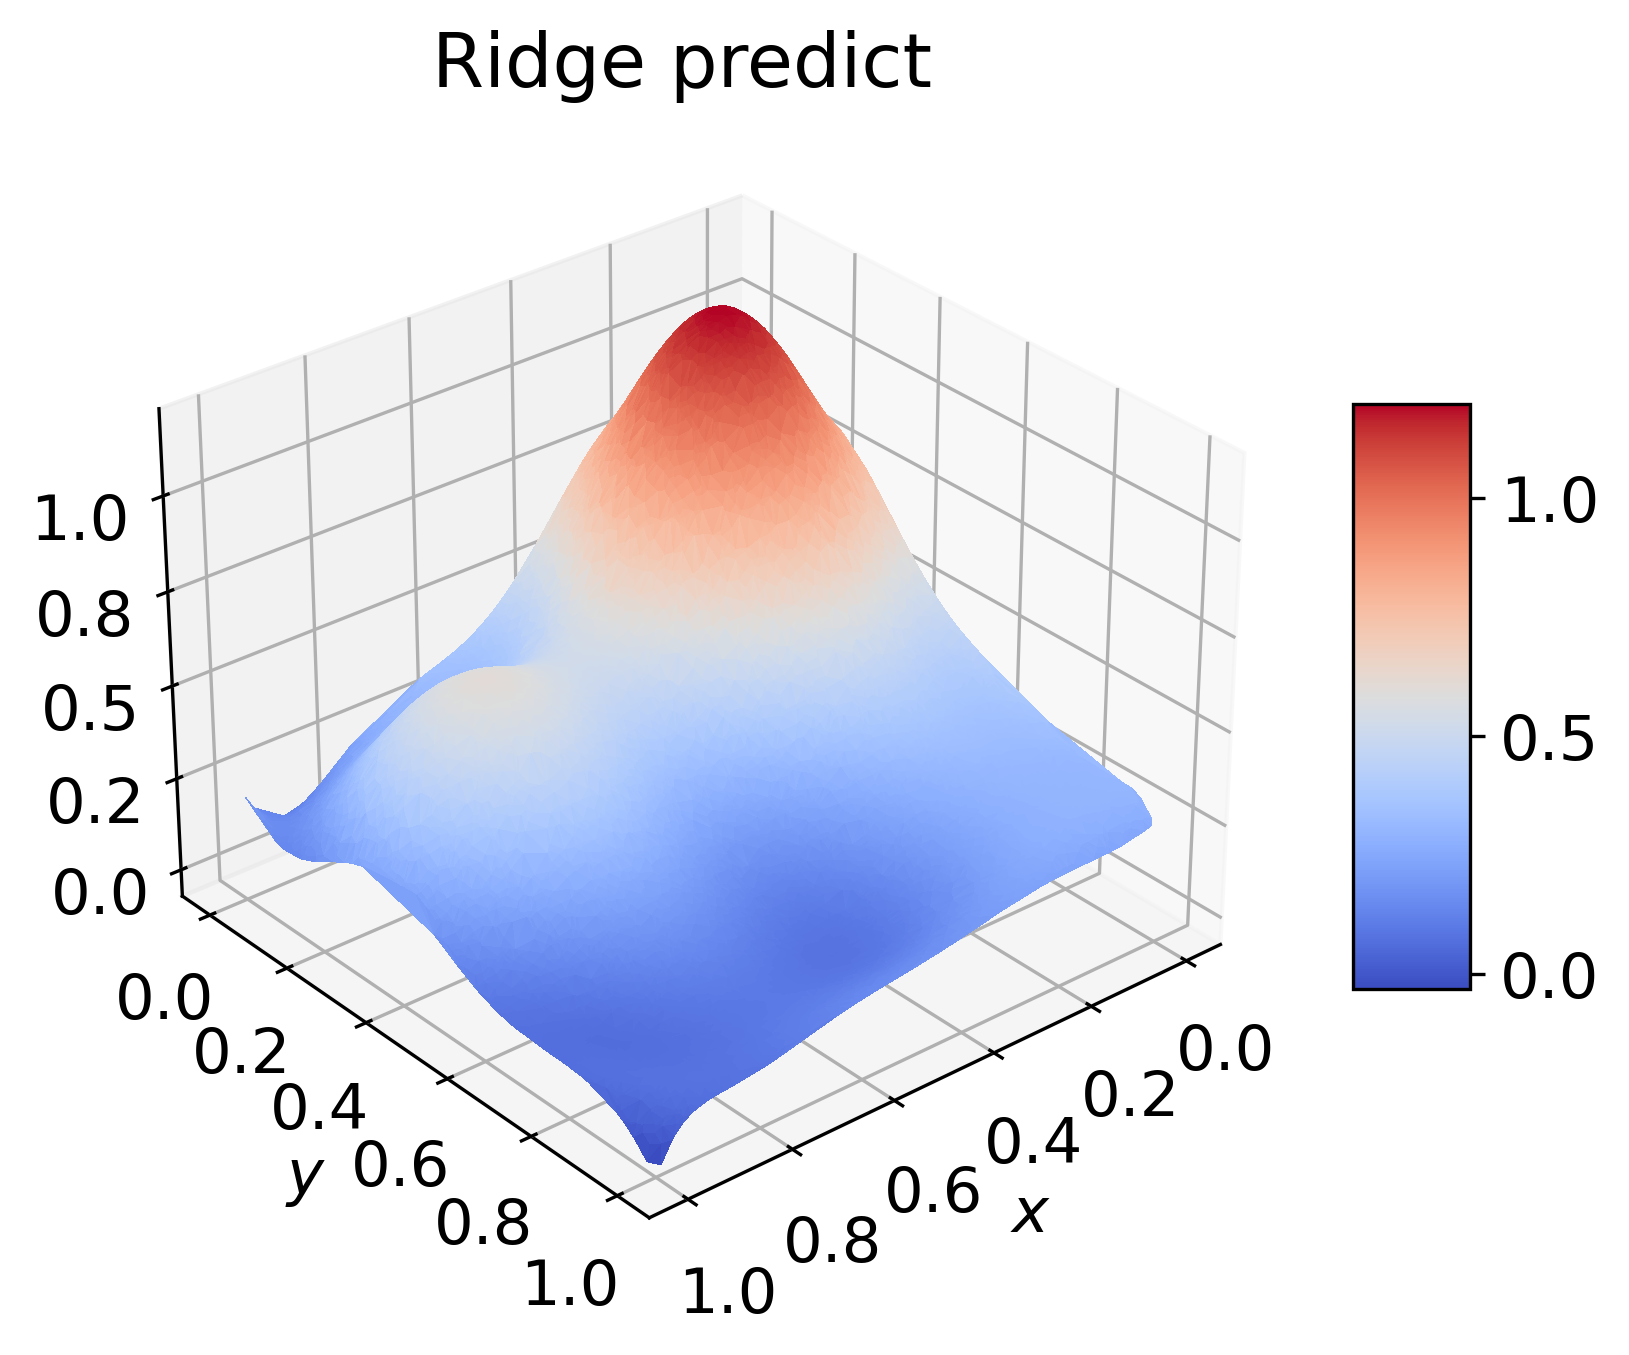
\includegraphics[width=\textwidth]{../figures/ridge_pred_franke_extra.png}
    \caption{Ridge prediction}
    \label{fig:extra_pred_ridge}
  \end{subfigure}
  \begin{subfigure}{.5\textwidth}
    \centering
    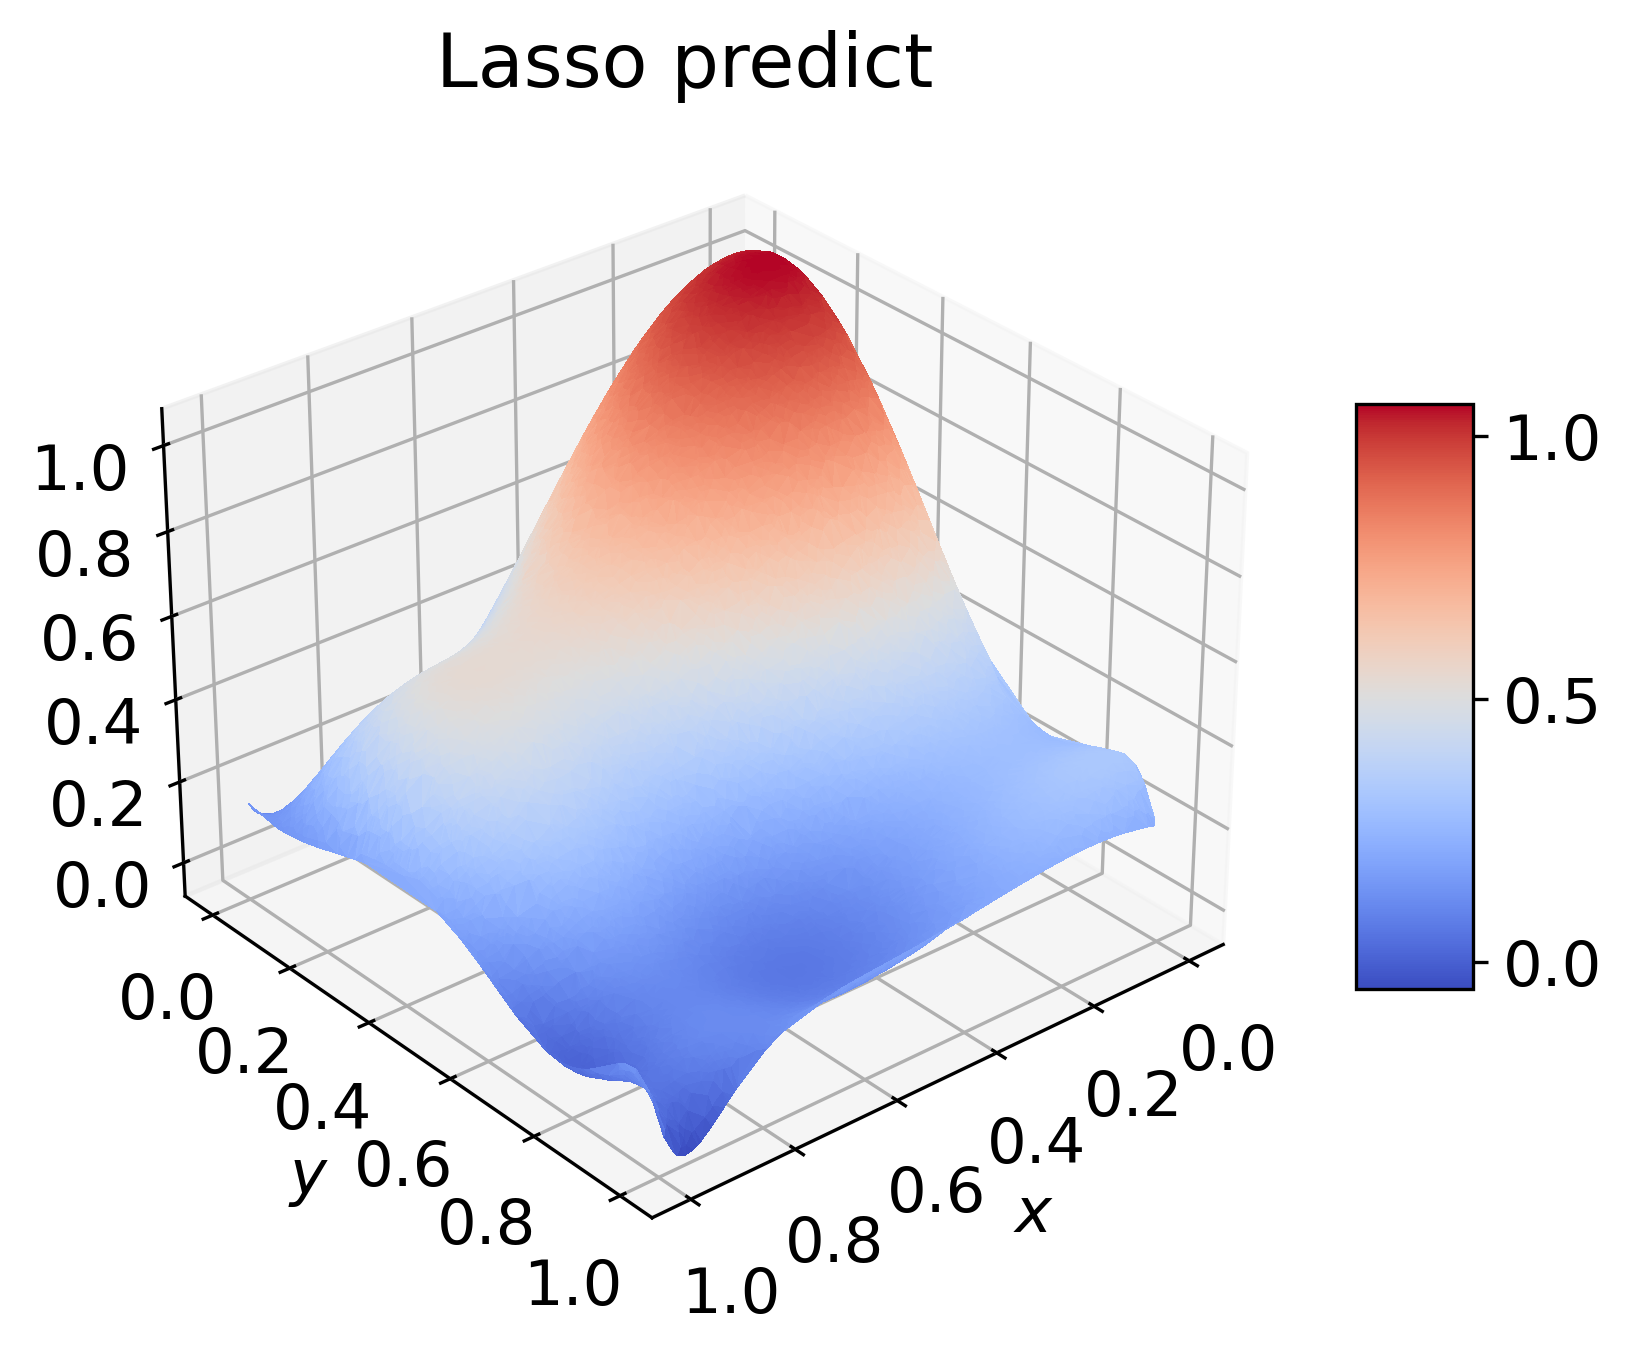
\includegraphics[width=\textwidth]{../figures/lasso_pred_franke_extra.png}
    \caption{Lasso prediction}
    \label{fig:extra_pred_lasso}
  \end{subfigure}
  \caption{Plot of the true Franke function together with our train and test data, and our predictions for our optimal parameters shown in table \ref{tab:best_comp} using $n=200$ steps and $\sigma=0.2$ }
  \label{fig:extra_pred_franke}
\end{figure}
We see in figure \ref{fig:pred_franke} that our predictions follow the general trend of the Franke function shown in figure \ref{fig:pred_real}. We see small differences between the 3 different predictions \ref{fig:pred_ols}, \ref{fig:pred_ridge}, and \ref{fig:pred_lasso}, but it remains hard to tell which does the best prediction without looking at table \ref{tab:best_comp}. Our plots are also quite choppy as a result of the small test sample. Here we have again used $n=30$ steps and a standard deviation of $\sigma=0.2$ which leaves us with an even smaller test sample and following resolution in our prediction plots.

Figure \ref{fig:extra_pred_franke} gives us a better visual understanding on how the regression methods perform using the parameters from \ref{tab:best_comp}. In total we see that both Rige and OLS are the ones who look most similar to the Franke function, which matches with what we saw in \ref{tab:best_comp}.
\subsection{Topography data}

We now look at real topography data and begin looking at how our OLS prediction reacts to design matrices of different polynomial degree, as shown for MSE and $R^2$ in figure \ref{fig:mse_r2_real}.
\begin{figure}[H]
  \begin{subfigure}{.5\textwidth}
    \centering
    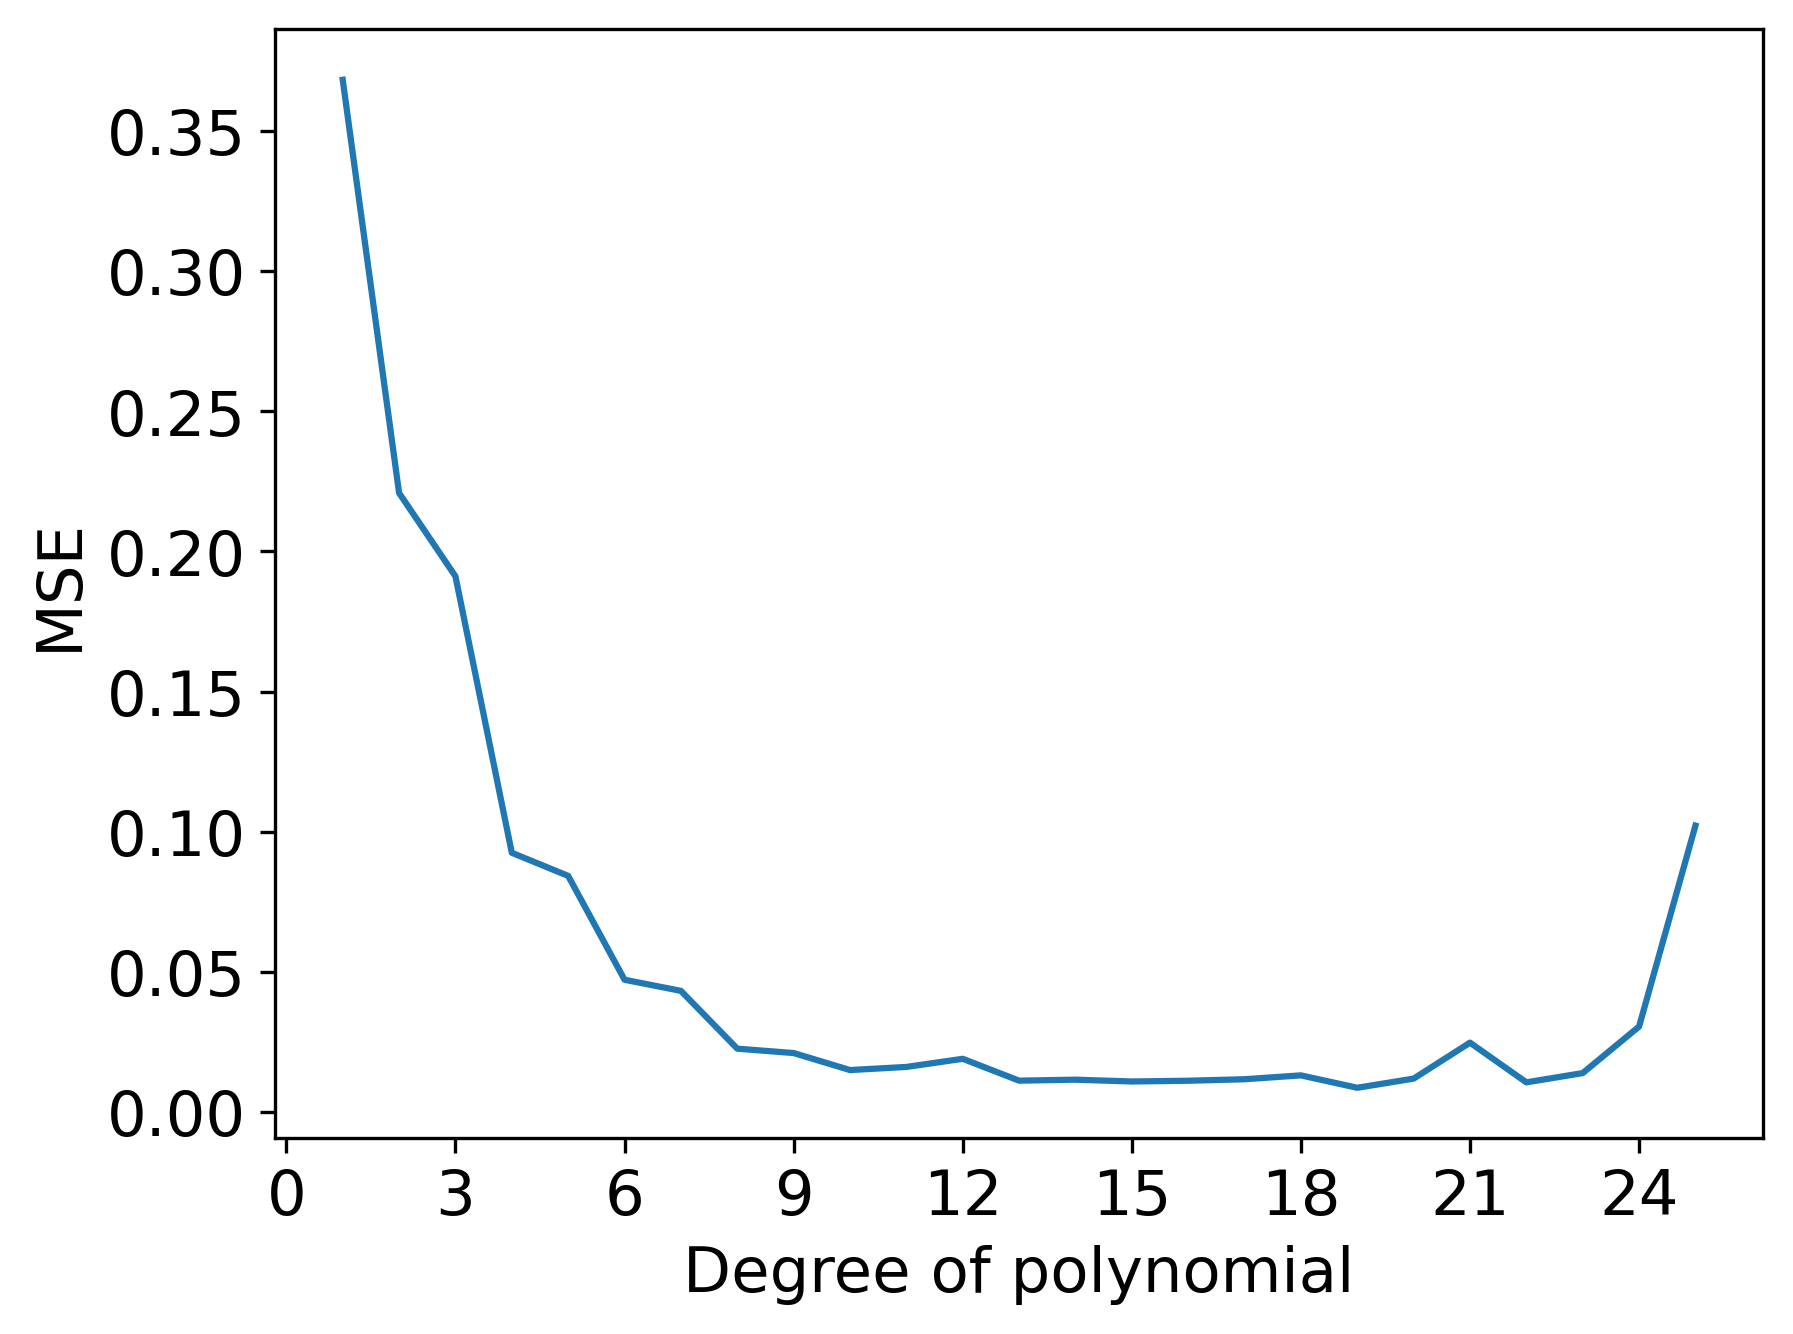
\includegraphics[width=\textwidth]{../figures/mse_deg_real.png}
    \caption{}
    \label{fig:}
  \end{subfigure}
  \begin{subfigure}{.5\textwidth}
    \centering
    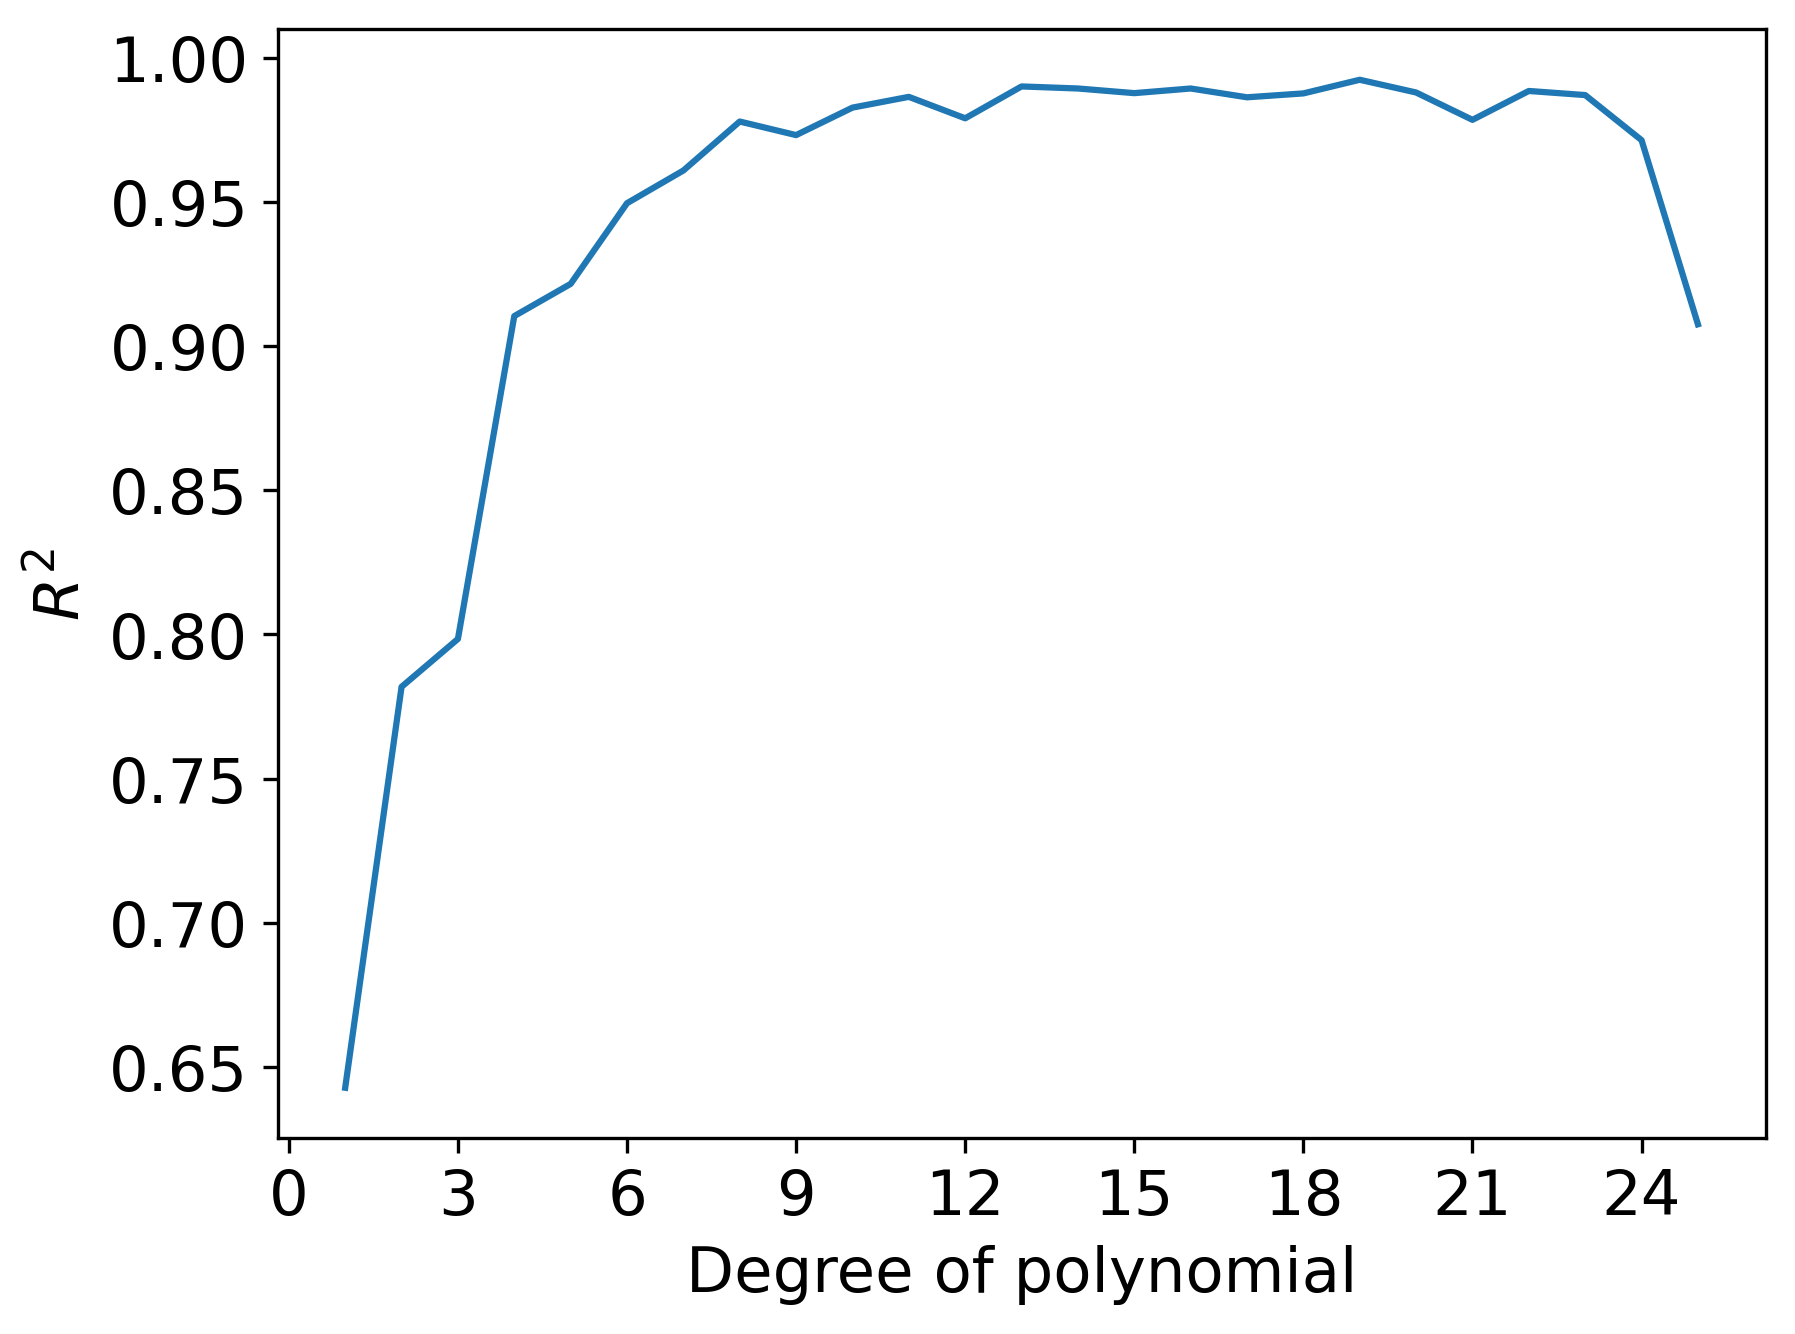
\includegraphics[width=\textwidth]{../figures/r2_deg_real.png}
    \caption{}
    \label{fig:}
  \end{subfigure}
  \caption{MSE and $R^2$ as a function of polynomial degree for OLS prediction. Here we are using indexes of [100:141] where every second index is skipped.}
  \label{fig:mse_r2_real}
\end{figure}
We see what seems like overfitting happening around a degree of 22 which is higher than what we saw for the Franke function. This indicates that we need a more advanced function to describe our data.

\subsubsection{The Bias-variance tradeoff}
We perform the bias variance tradeoff for the three methods for a degree up to 25, and for ridge and lasso also different $\lambda$ parameters. OLS in figure \ref{fig:tradeoff_real}, Ridge in figure \ref{fig:ridge_tradeoff_real} and Lasso in figure \ref{fig:lasso_tradeoff_real}
\begin{figure}[H]
  \centering
  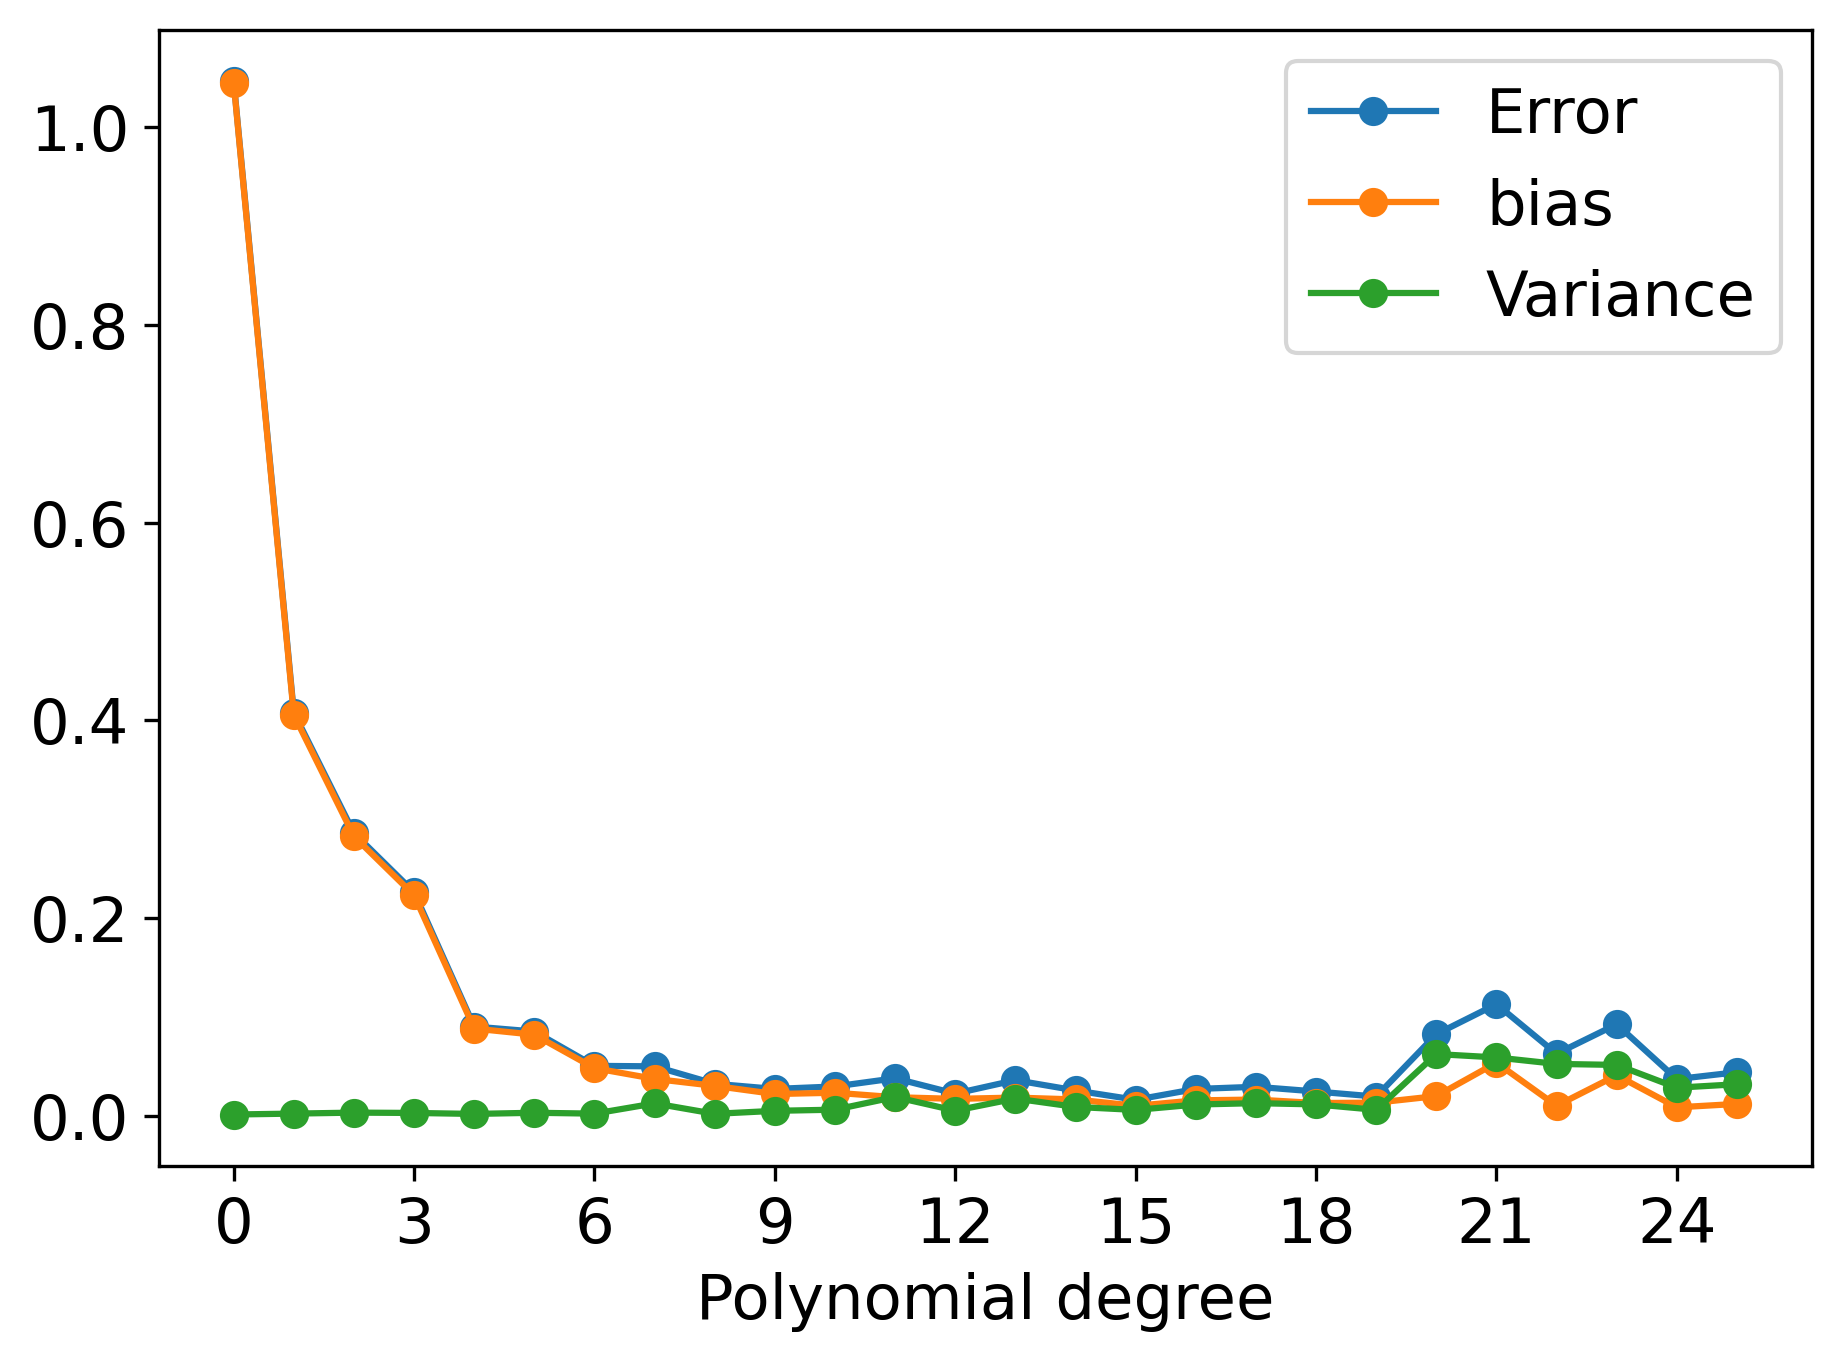
\includegraphics[width=.4\textwidth]{../figures/ols_real_tradeoff.png}
  \caption{Bias-variance tradeoff for the OLS method}
  \label{fig:tradeoff_real}
\end{figure}

\begin{figure}[H]
  \begin{subfigure}{.5\textwidth}
    \centering
    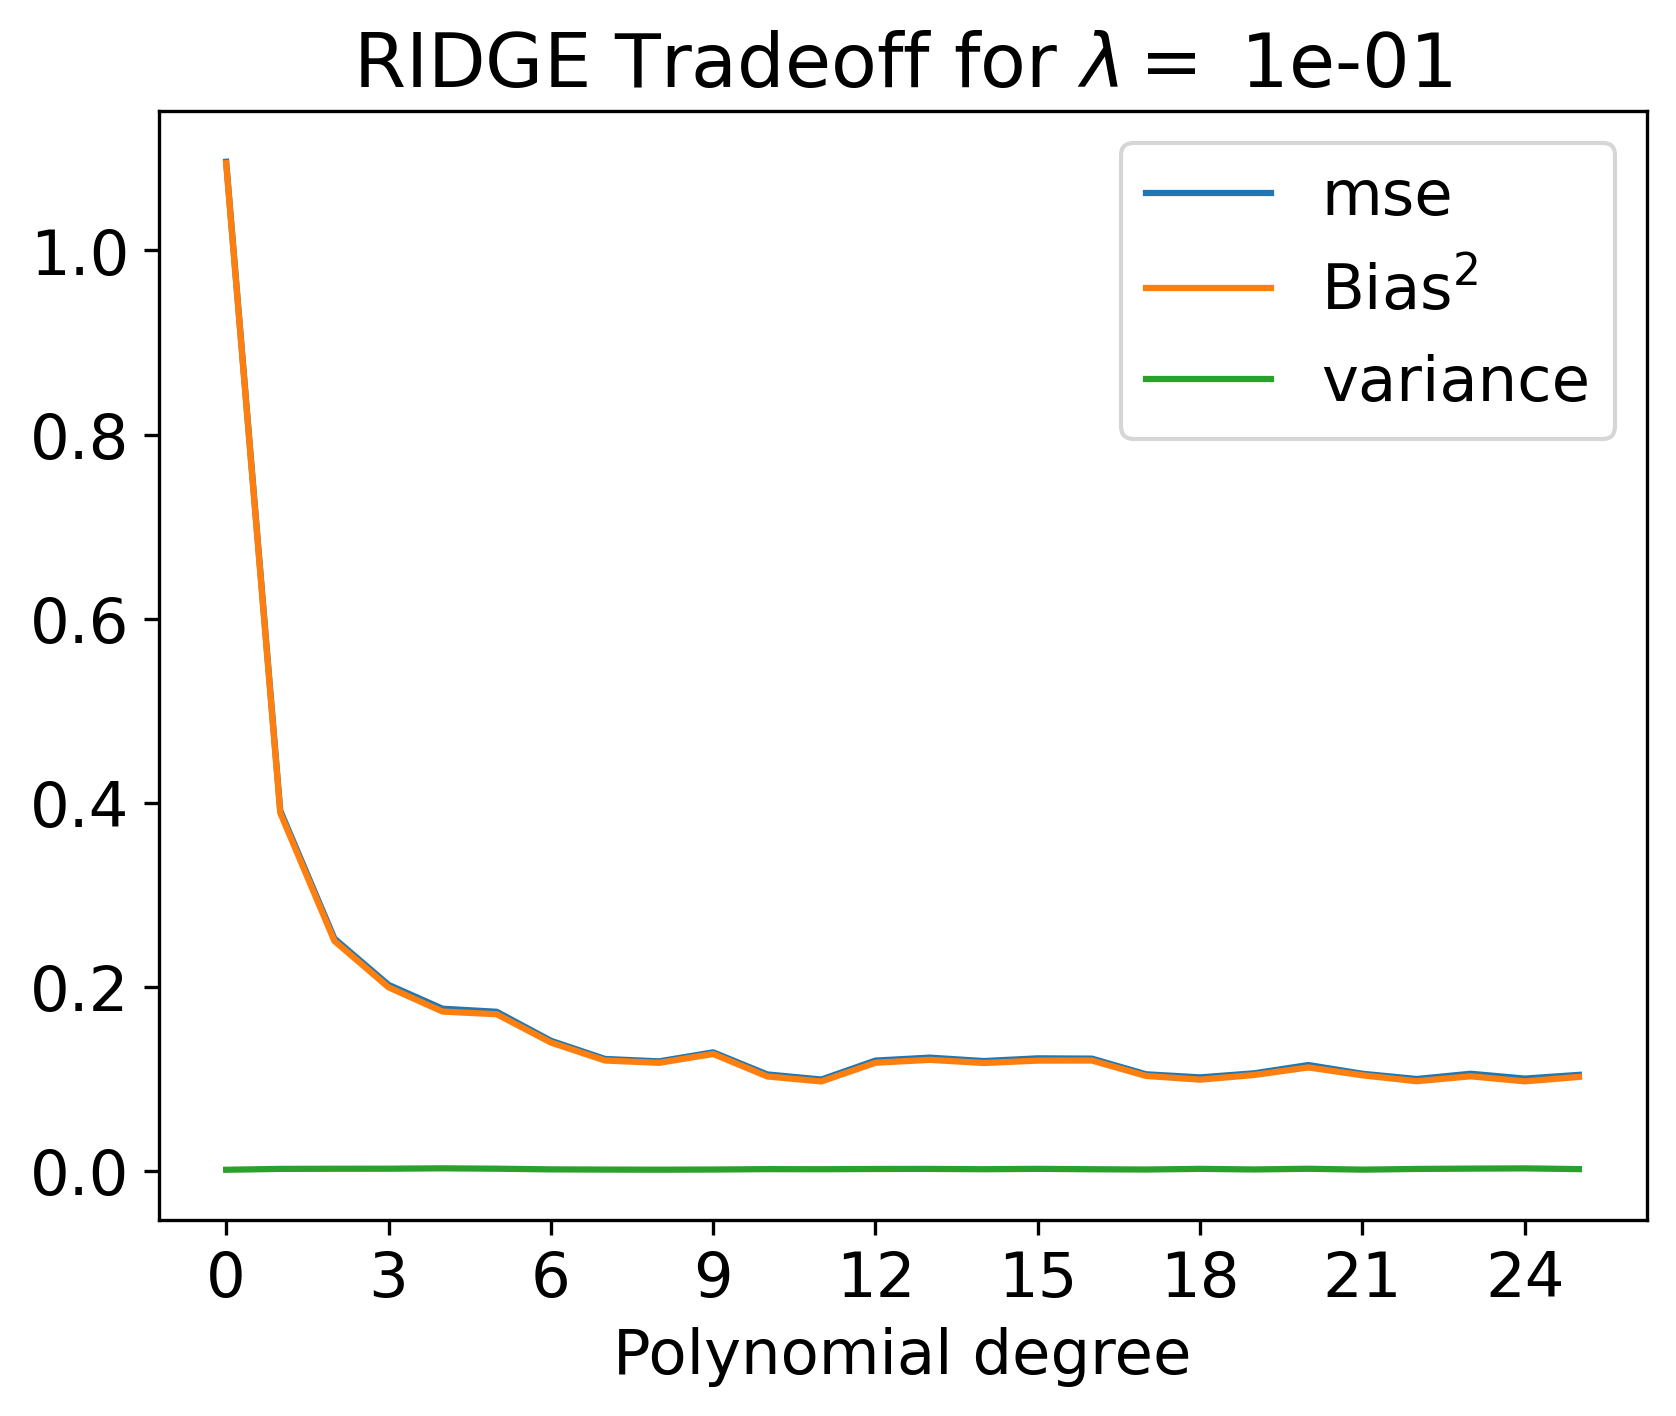
\includegraphics[width=.8\textwidth]{../figures/tradeoff_RIDGE_1e-01real.png}
    \caption{}
    \label{fig:}
  \end{subfigure}
  \begin{subfigure}{.5\textwidth}
    \centering
    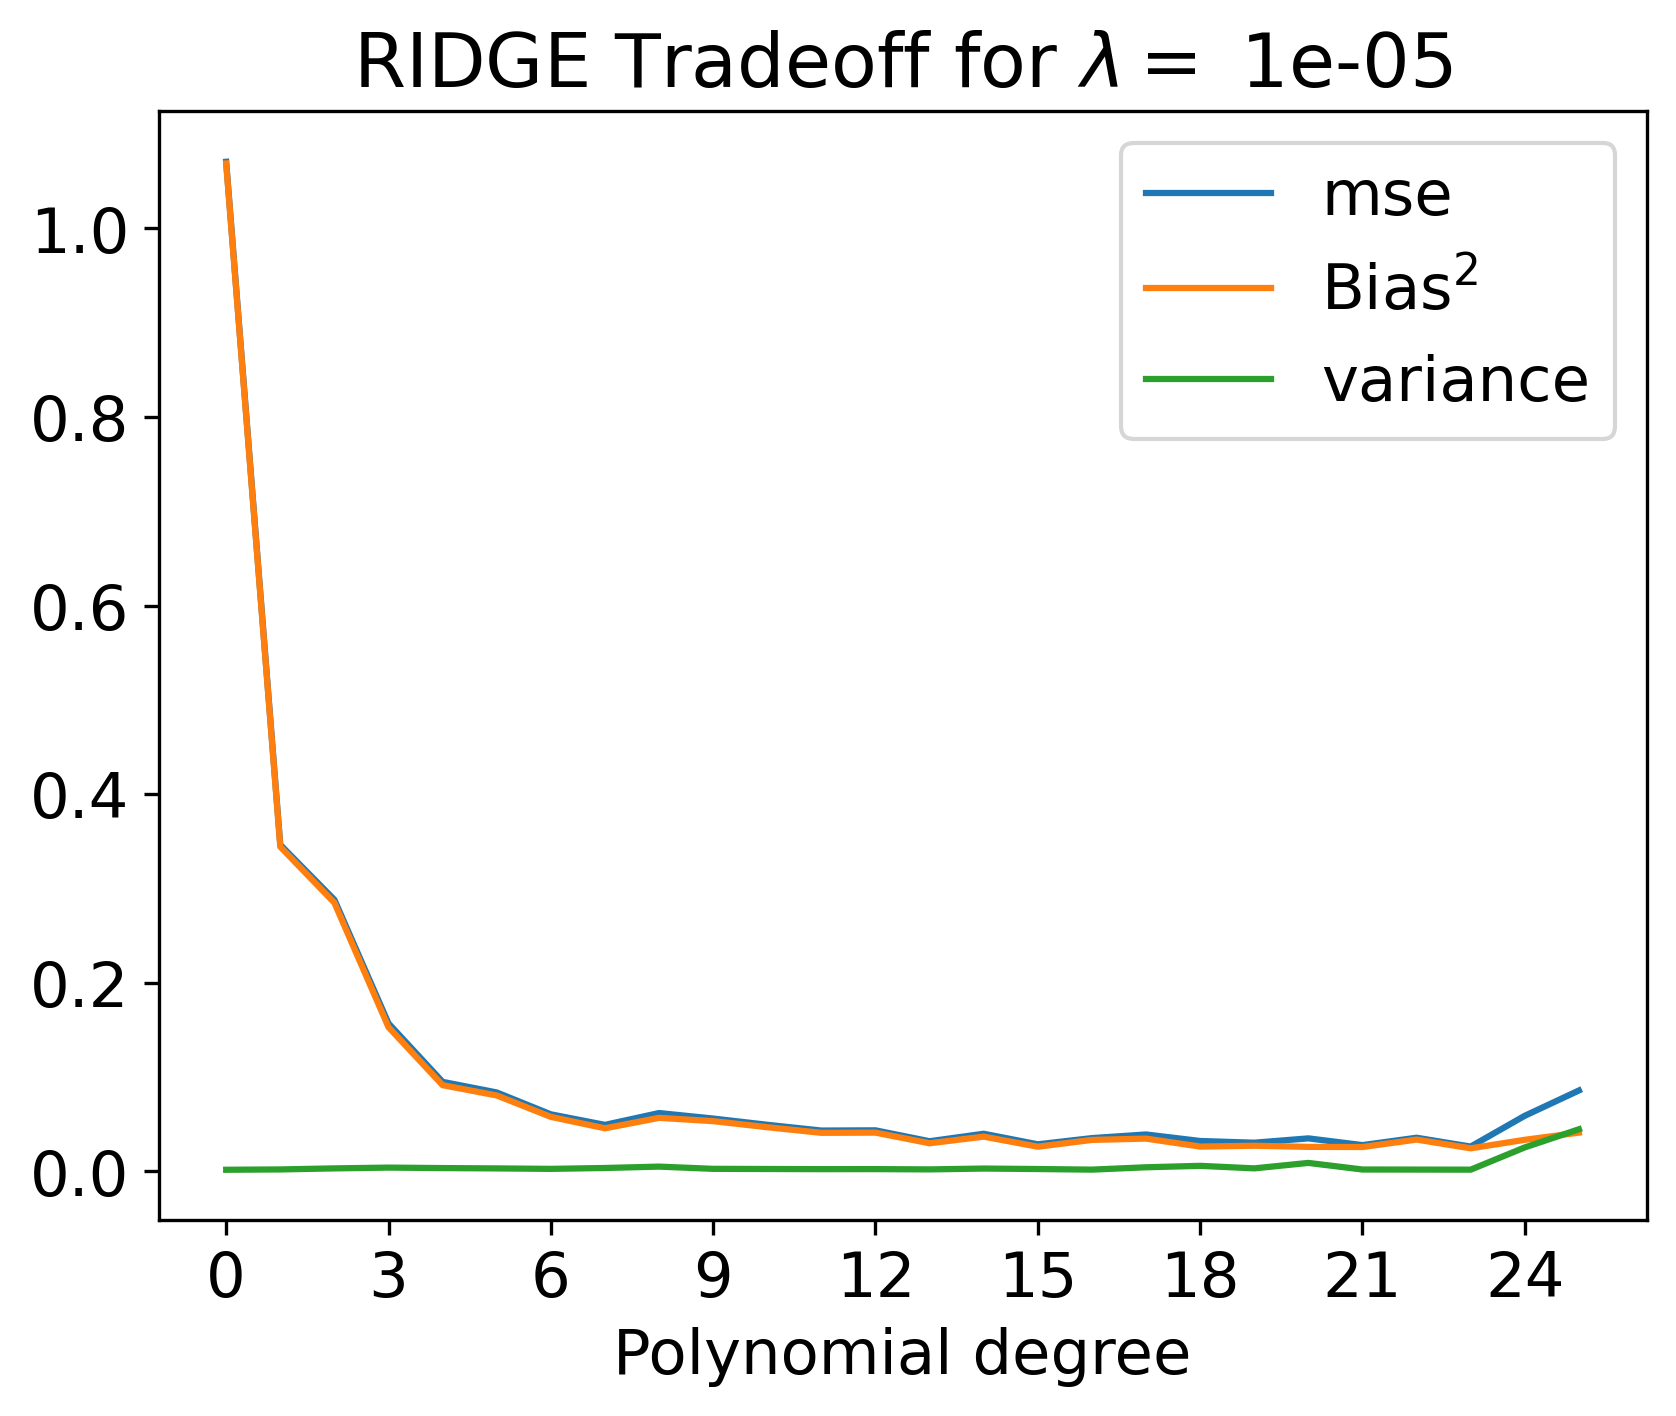
\includegraphics[width=.8\textwidth]{../figures/tradeoff_RIDGE_1e-05real.png}
    \caption{}
    \label{fig:}
  \end{subfigure}
  \begin{subfigure}{.5\textwidth}
    \centering
    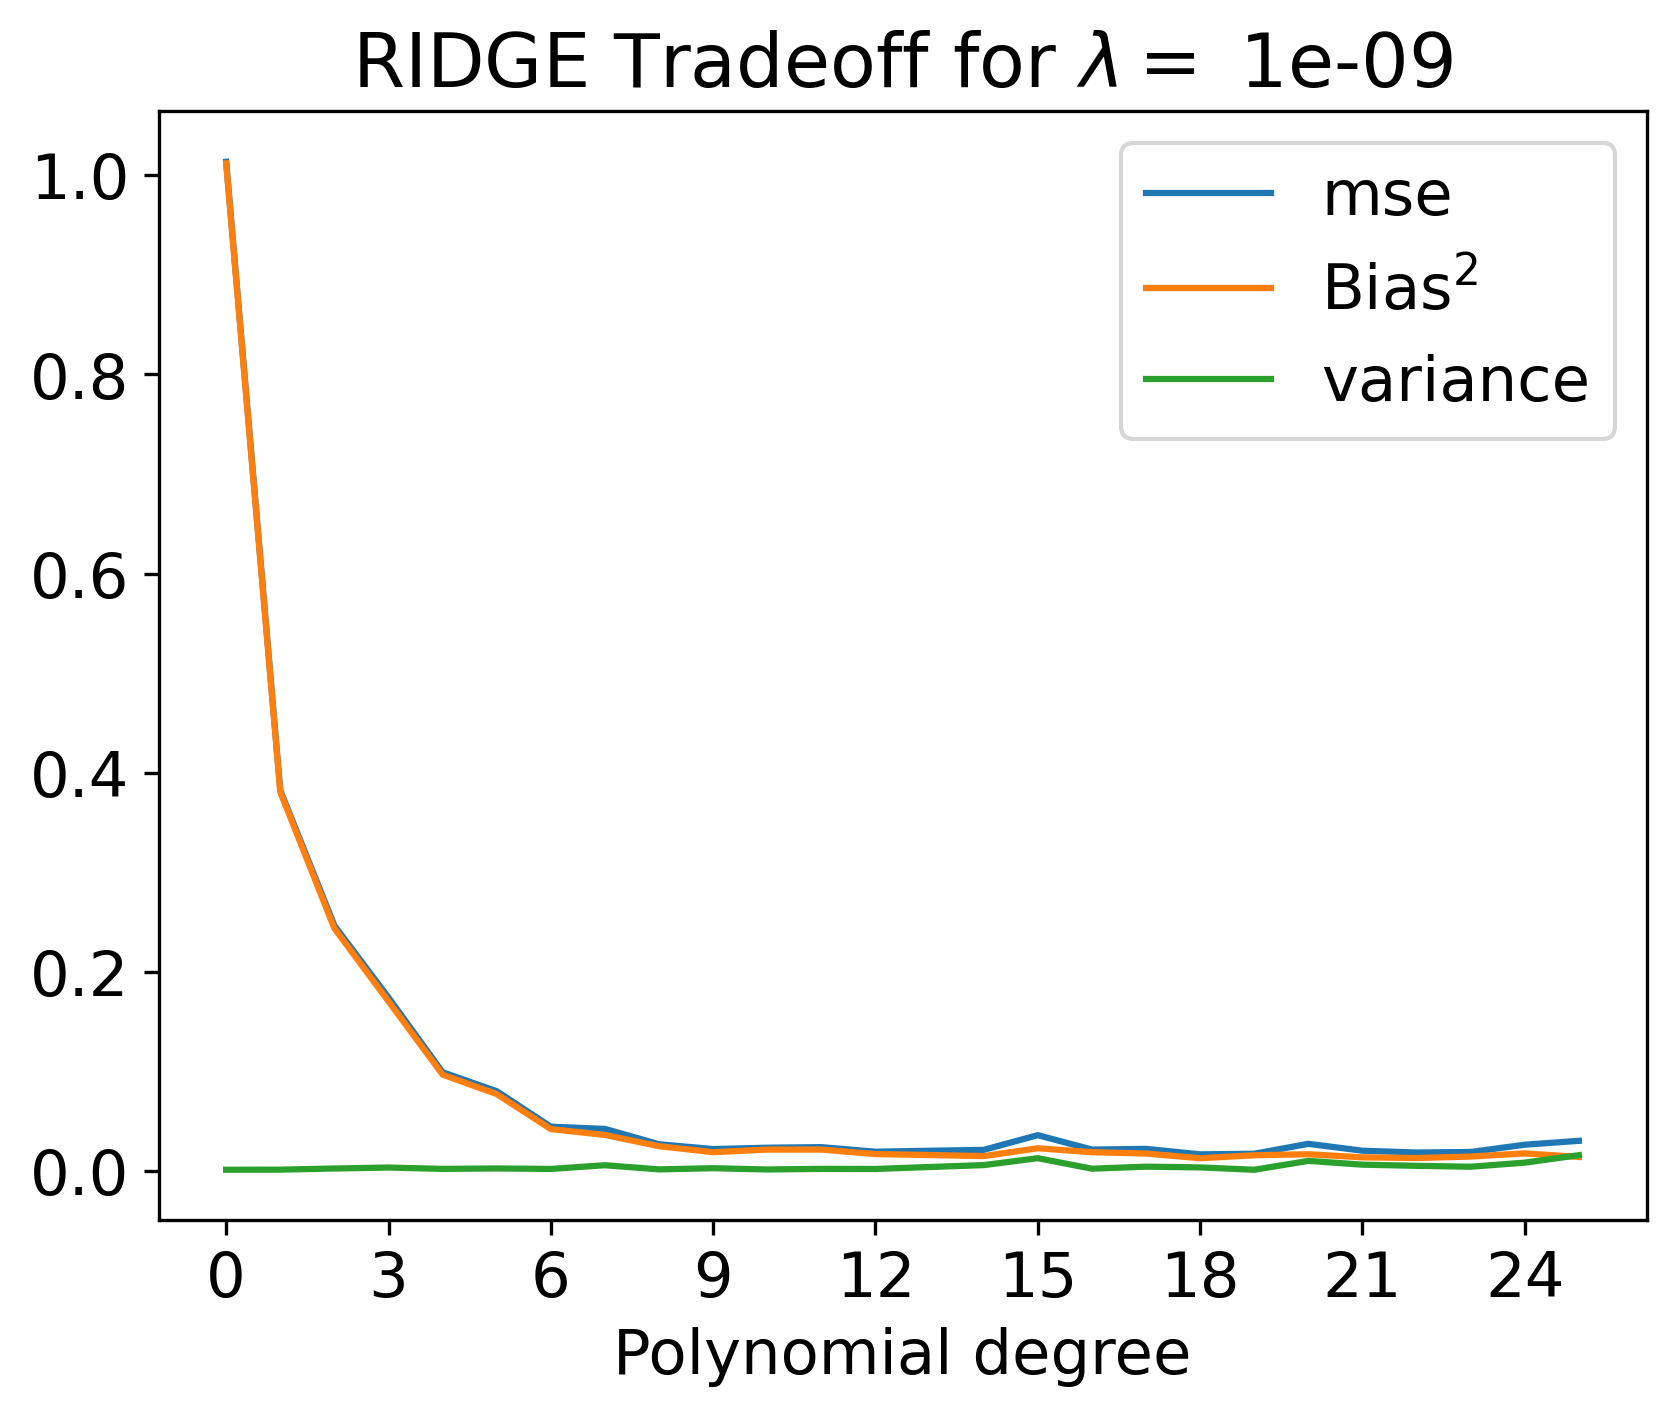
\includegraphics[width=.8\textwidth]{../figures/tradeoff_RIDGE_1e-09real.png}
    \caption{}
    \label{fig:}
  \end{subfigure}
  \begin{subfigure}{.5\textwidth}
    \centering
    \includegraphics[width=.8\textwidth]{../figures/tradeoff_RIDGE_1e-13real.png}
    \caption{}
    \label{fig:}
  \end{subfigure}
  \caption{Bias-variance tradeoff for different choices of lambda using Ridge regression}
  \label{fig:ridge_tradeoff_real}
\end{figure}

\begin{figure}[H]
  \begin{subfigure}{.5\textwidth}
    \centering
    \includegraphics[width=\textwidth]{../figures/tradeoff_LASSO_1e-01real.png}
    \caption{}
    \label{fig:}
  \end{subfigure}
  \begin{subfigure}{.5\textwidth}
    \centering
    \includegraphics[width=\textwidth]{../figures/tradeoff_LASSO_1e-05real.png}
    \caption{}
    \label{fig:}
  \end{subfigure}
  \begin{subfigure}{.5\textwidth}
    \centering
    \includegraphics[width=\textwidth]{../figures/tradeoff_LASSO_1e-09real.png}
    \caption{}
    \label{fig:}
  \end{subfigure}
  \begin{subfigure}{.5\textwidth}
    \centering
    \includegraphics[width=\textwidth]{../figures/tradeoff_LASSO_1e-13real.png}
    \caption{}
    \label{fig:}
  \end{subfigure}
  \caption{Bias-variance tradeoff for different choices of lambda using Lasso regression}
  \label{fig:lasso_tradeoff_real}
\end{figure}
We see that OLS keeps a low variance until a degree of 19 while the bias generally stays low for degrees of around 8 and above. For Ridge and Lasso we see the same trend as for OLS with a decreasing bias for greater degrees. On the other hand we do not notice any significant increase in the variance for both lasso and Ridge which we can see in the OLS tradeoff. We also see that Ridge keeps a low variance up to a degree of at least 20 for different values of $\lambda$, while Lasso keeps the variance low for any choices of $\lambda$ which means that the bias has the main responsibility for the MSE of these models.

\subsubsection{Finding best models}
To find the optimal model we do as for the Franke function plot a heatmap to find for which $\lambda$ and degree we get the lowest MSE as seen in figure \ref{fig:heat_real}.
\begin{figure}[H]
  \begin{subfigure}{\textwidth}
    \centering
    \includegraphics[width=.5\textwidth]{../figures/best_lambda_OLS_00.png}
    \caption{OLS}
    \label{fig:best_ols_real}
  \end{subfigure}\\[1ex]
  \begin{subfigure}{.5\textwidth}
    \centering
    \includegraphics[width=\textwidth]{../figures/best_lambda_RIDGE_00.png}
    \caption{Ridge}
    \label{fig:best_ridge_real}
  \end{subfigure}
  \begin{subfigure}{.5\textwidth}
    \centering
    \includegraphics[width=\textwidth]{../figures/best_lambda_LASSO_00.png}
    \caption{Lasso}
    \label{fig:best_lasso_real}
  \end{subfigure}
  \caption{Heatmap of MSE for different choices of polynomial degree and $\lambda$. Here we have used cross validation with 5$k$-folds for data of indexes [100:141] where every second index is skipped}
  \label{fig:heat_real}
\end{figure}
We see in \ref{fig:best_ols_real} that the OLS generally gives low MSE from around a degree of 12 until a degree of 25 where the MSE blows up. For Ridge in \ref{fig:best_ridge_real} we see that a quite low $\lambda$ is required together with a degree of at least 12. In total the parameter $\lambda =3.79 \times 10^{-12}$ together with a degree of 20 ends up giving the lowest MSE. For Lasso in figure \ref{fig:best_lasso_real} we see that the model is not so strict on what $\lambda$ it takes in but rather the degree. We see lower MSE from a degree of around 25 matched up with a $\lambda$ of $10^{-5}$ or lower. In total we see that a degree of 29 together with a parameter $\lambda=1.23\times10^{-10}$ gives the lowest MSE. But at the same time we can notice that the MSE for Lasso is on another scale than for Ridge and OLS, which indicates the Lasso method performing worse in this case. The best parameters, degrees and MSEs can be seen under in table \ref{tab:best_comp_real}
\begin{table}[H]
  \centering
  \caption{Table of best parameters and the following MSE for OLS, Ridge and Lasso regression}
  \label{tab:best_comp_real}
  \begin{tabular}{|c||c|c|c|}
    \hline
    Method & $\lambda$ & Degree & $MSE$ \\
    \hline
    OLS &  & 19 & 0.0107 \\
    \hline
    RIDGE & $3.79\times10^{-12}$ & 20 & 0.0100 \\
    \hline
    LASSO & $1.23\times10^{-10}$ & 29 & 0.0682 \\
    \hline
  \end{tabular}
\end{table}
We see above in table \ref{tab:best_comp_real} that Ridge barely beats OLS and again that Lasso is quite far behind them both.
\subsubsection{Predictions}
From the best parameters we found in figure \ref{fig:heat_real} we make predictions and plot them as seen in figure \ref{fig:pred_real_skip}. To plot a smoother surface we can also use the same parameters as seen in table \ref{tab:best_comp_real} without skipping every second step in the terrain data. This gives us more data points to train and predict on, giving us figure \ref{fig:real_pred}.


\begin{figure}[H]
  \begin{subfigure}{.5\textwidth}
    \centering
    \includegraphics[width=\textwidth]{../figures/actual_data_n40_skip2.png}
    \caption{Full data before split}
    \label{fig:real_pred_real_skip}
  \end{subfigure}
  \begin{subfigure}{.5\textwidth}
    \centering
    \includegraphics[width=\textwidth]{../figures/train_data_n40_skip2.png}
    \caption{Train data from function data with added noise}
    \label{fig:real_pred_train_skip}
  \end{subfigure}
  \begin{subfigure}{.5\textwidth}
    \centering
    \includegraphics[width=\textwidth]{../figures/test_data_n40_skip2.png}
    \caption{Test data from function data with added noise}
    \label{fig:real_pred_test_skip}
  \end{subfigure}
  \begin{subfigure}{.5\textwidth}
    \centering
    \includegraphics[width=\textwidth]{../figures/ols_pred_n40_skip2.png}
    \caption{OLS prediction}
    \label{fig:real_pred_ols_skip}
  \end{subfigure}
  \begin{subfigure}{.5\textwidth}
    \centering
    \includegraphics[width=\textwidth]{../figures/ridge_pred_n40_skip2.png}
    \caption{Ridge prediction}
    \label{fig:real_pred_ridge_skip}
  \end{subfigure}
  \begin{subfigure}{.5\textwidth}
    \centering
    \includegraphics[width=\textwidth]{../figures/lasso_pred_n40_skip2.png}
    \caption{Lasso prediction}
    \label{fig:real_pred_lasos_skip}
  \end{subfigure}
  \caption{Plot of our data together with our train and test data, and our predictions for our optimal parameters shown in table \ref{tab:best_comp_real} }
  \label{fig:pred_real_skip}
\end{figure}

\begin{figure}[H]
  \begin{subfigure}{.5\textwidth}
    \centering
    \includegraphics[width=\textwidth]{../figures/actual_data_n40.png}
    \caption{Full data before split}
    \label{fig:real_pred_real}
  \end{subfigure}
  \begin{subfigure}{.5\textwidth}
    \centering
    \includegraphics[width=\textwidth]{../figures/train_data_n40.png}
    \caption{Train data from function data with added noise}
    \label{fig:real_pred_train}
  \end{subfigure}
  \begin{subfigure}{.5\textwidth}
    \centering
    \includegraphics[width=\textwidth]{../figures/test_data_n40.png}
    \caption{Test data from function data with added noise}
    \label{fig:real_pred_test}
  \end{subfigure}
  \begin{subfigure}{.5\textwidth}
    \centering
    \includegraphics[width=\textwidth]{../figures/ols_pred_n40.png}
    \caption{OLS prediction}
    \label{fig:real_pred_ols}
  \end{subfigure}
  \begin{subfigure}{.5\textwidth}
    \centering
    \includegraphics[width=\textwidth]{../figures/ridge_pred_n40.png}
    \caption{Ridge prediction}
    \label{fig:real_pred_ridge}
  \end{subfigure}
  \begin{subfigure}{.5\textwidth}
    \centering
    \includegraphics[width=\textwidth]{../figures/lasso_pred_n40.png}
    \caption{Lasso prediction}
    \label{fig:real_pred_lasso}
  \end{subfigure}
  \caption{Plot of our data together with our train and test data, and our predictions for our optimal parameters shown in table \ref{tab:best_comp_real}. Here is our data size larger than what shown in figure \ref{fig:pred_real_skip} but from the same source to give a better visual understanding of our predictions.}
  \label{fig:real_pred}
\end{figure}
As we can see in figure \ref{fig:pred_real_skip} we get for all the regression methods low resolution results. We see that using terrain data without skipping every second index as shown in figure \ref{fig:real_pred} gives us higher resolution. This gives us the possibility to visualize a greater difference between the three models. We can see that OLS and Ridge predict the small bumps in the farthest corner in \ref{fig:real_pred_real} while lasso smooths them out to one top as seen in \ref{fig:real_pred_lasso}.
\section{Discussion}
\subsection{Scaling of data}
Our result from our comparison between scaled and non-scaled data from the Franke function (\ref{fig:compare_scale}) showed that further scaling was unnecessary. But the choice of not scaling could have made our results inaccurate, especially for Ridge and Lasso regression where the magnitude of the coefficient for one variable is dependent on the magnitude of that variable. We see in figure \ref{fig:compare_scale} that this may especially be true for design matrices of higher degrees where the differences between scaled and non-scaled data in both MSE and $R^2$ increases. For models like Ridge and Lasso which have a regularization that makes higher polynomial degrees more favorable would therefore especially take an accuracy hit to their full potential for the choice of not scaling.

For our topography data we ended up scaling our $z$-values but not our chosen design matrix with $x,y\in [0,1]$. This may similar to the Franke function have given us an unnecessary amount of implications while using scikit-learn's lasso implementation. Here we saw a convergence problem in our code, which could have been avoided by scaling of our data. Another scaling method which restricts the scaled data to an interval could also have been a solution. Standard scaling does not do this and can leave us with scaled data with magnitudes of more than 1. This may be the reason of our Lasso method performing much better for the Franke function which already have maximum $z$ values just above 1. An increase in the number of maximum iterations for the Lasso method is also a solution to fix the convergence problem but at a great cost of computation time. Without a powerful enough computer we were restricted to either choose a maximum number of iterations to 100 or 1000 which may be an explanation to why the lasso method performed worse for both the Franke function \ref{tab:best_comp} and especially for real data \ref{tab:best_comp_real}.

\subsection{Splitting of data and overfitting}
As we saw in figure \ref{fig:train_test_resample_mse} and \ref{fig:train_test_resample_r2}, it is clear that we for higher degrees start seeing overfitting. Here it is important to notice that our plots are a result of pulling more samples from the same distribution, which is not what we normally can perform in a real life scenario. These figures serves therefore only a purpose of showing how we will always gain a lower MSE by predicting using our train data. This is the main reason why we perform a train-test split of our data when performing all our analysis. That means we will not only adjust our model to fit the data we have at hand, but also predict other data which comes from the same source. Therefore the test data serves the purpose of reducing overfitting.

When we look at the bias variance tradeoff in figure \ref{fig:bias_variance} we see the same trend as in figure \ref{fig:train_test_resample_mse}. A lower MSE for around a degree of 6 and a following increase for higher and lower degrees. What is interesting here is that we gain an insight into what is causing the errors at different degrees. As we described earlier in the method part of this report, the MSE is a function of the bias, variance and the standard deviation of the noise. From this it is expected that a larger bias as a result of the simplification of our model by using lower degrees is the main contributor to the error for low degrees. Following we also see how the increase in polynomial degree causes an increase in variance. This is a sign of overfitting showing our model's variance by training it with different datasets.

\subsection{Comparison of bootstrap and cross validation}
In our comparison between bootstrap and cross validation in figure \ref{fig:cv_comp}, we saw a trend of bootstrap giving lower MSE for lower polynomial degrees while cross validation gave us lower MSE for higher degrees. When we compare the two choices of $k$-folds we see a smoother plot for 10 $k$-folds and otherwise a slightly lower MSE for higher degrees. This means that a higher choice of $k$-folds when performing an analysis of best polynomial degree, could change our results for an optimal model to one with higher variance and lower bias. When continuing our analysis we have used a $k$-fold of 5 which means our models would favor a higher bias and lower variance. This is often a useful choice when we have limited data which is the case for us. At the same time, research has suggested that more advanced models which would be considered overfitted, also have a high accuracy on test data \cite{overfitting}. This means that we are always left with a hard choice when choosing the right amount of $k$-folds in our cross validation, which means this is an interesting topic for further research.

\subsection{Choice of $\lambda$ parameters}
A further inaccuracy in the results from our models may have come from our choice of $\lambda$ parameters we tested for. Here is both the amount of parameters and the interval of parameters we tested for a possible error to our methods. For example could a $\lambda$ we did not test to make the Lasso method the method with best predictions for the Franke function. This means that there is a great room for improvement in our choice of $\lambda$ parameters, but in the end will the right choice of $\lambda$ forever be a question while we will always be restricted on the computational power we have at hand.

\subsection{Predictions}
For the Franke function we found that Ridge barely gave us the prediction with the lowest MSE right in front of OLS, which as discussed earlier could have been the other way around if tested for different $\lambda$ parameters. We also saw in figure \ref{fig:heat_franke} that we have different axis of both $\lambda$ and polynomial degrees as a result of the Lasso regression generally requiring both smaler values of $\lambda$ and higher polynomial degrees to do its best predictions. We saw this quite clear in figure \ref{fig:beta_lambda_rl}, and is a result of the Lasso method being more aggressive when regularizing the $\beta$ parameters by easily putting them to 0 in contradiction to Ridge which has its parameters following a function of $\lambda$. This means that we for Lasso can get away with higher polynomial degrees because the parameters that for another method would get big, may for Lasso go towards 0 and in that way reduce overfitting. For Ridge it may go towards a small number but never 0. This means that overfitting would generally happen for lower polynomial degrees when using Ridge than when using Lasso.

In \ref{fig:extra_pred_franke} we made further predictions on a new dataset starting with the optimal parameters found in table \ref{tab:best_comp} to get a better visual understanding of our predictions. Here we have not stored the beta parameters computed earlier for $n=30$ which means that new parameters have been computed. This is typically not what you would do in a real world scenario when you gain new data to test for. For this increase in steps to $n=200$ it would be beneficial to find new optimal parameters which would because of an increase in sample size end up making better predictions. This means that this plot does not tell us anything special but rather shows us that the parameters shown in \ref{tab:best_comp} would give us a good understanding of where we should start with our analysis given a new and bigger dataset from the same source.

What discussed above is also valid for our plot \ref{fig:real_pred} which means that these also are only left as nice looking visualizations and not necessarily telling us anything about our methods. Furthermore are our predictions in this case not made based on some function with some large noise. This means that our predictions may be worse than our initial data at describing the topography depending on how accurate our topography measurements are. For sea level height data measured by remote sensing it is found that uncertainties in measurements of local change in sea level height are as low as 0.062mm/year \cite{sealevel} which leaves us to believe that similar surface height measurements of topography has an uncertainty of the same scale. This means that the predictions performed on our topography data serves only as a study of how different regression methods predicts and reacts to different input data. What would on the other hand be interesting to do to with our topography data, is to see if a trained model on one surface could help to make a prediction on another where there is less available data or data of lower quality or resolution. Such an analysis we have not looked into in this report and is therefore left as a possibility for further research.

\section{Conclusion}
In total we have looked at both generated data from the Franke function and real topography data. Both have ended up being more of a study of our three different regression methods, OLS, Lasso and Ridge, than a study of the data in itself. We have implemented the two resampling methods cross validation and bootstrap and used these for an analysis of both the bias variance tradeoff and a mean squared error analysis. We have found that Ridge regression gives the best results in both our cases, scoring a slightly lower MSE than ordinary least squares. We have seen that Lasso regression generally predicts worse than both OLS and Ridge, and we have seen that this may in fact be as a result of our implementation of the method and not the nature of the method itself. We were limited in computational power and made a choice of not always fully scale or choosing the standard scaling method instead of a method keeping the magnitudes less than 1 which may have had great cost to the Lasso methods performance. This means that a scaled, more accurate and higher resolution analysis of our three regression methods could give us an even better understanding of the performance of our three regression methods. Therefore can we say that there is room for further analysis of these methods. Even though we in this case only have looked into the regression methods themselves, we have also found room for possible further research in terms of topography height predictions. If of interest could a trained model of a specific topography type be used to predict an area of similar topography where we have a lack of, or bad quality data.
\newpage
\nocite{bishop}
\nocite{hastie}
\printbibliography
\end{document}
